\chapter{Observation Simulation}\label{ch:obs_sims}

Along with improvements in instrumentation and data analysis, the planet-finding community has also devoted resources to the development of detailed models and simulations of the various instruments and surveys currently in operation.  These simulations serve three main purposes:  first, they allow the community to directly compare the expected scientific returns of proposed observatory and mission concepts \citep{savransky2010}.  Second, these simulations can be used to optimize target selection and observation scheduling for existing facilities, and provide a controlled testing environment for data processing pipelines \citep{bryson2010kepler}. Finally, by simulating a planet population derived from a specific formation/evolution theory, we can estimate the likelihood of survey results, and thus accept or reject the theory, while also closely estimating absolute planet frequencies \citep{gould2010frequency}.  This last capability translates to the ability to use surveys as controlled experiments to choose between competing exosystem formation and evolution theories.  The ability to predict the expected science returns of a proposed architecture is particularly important given the resources required to operate a major ground-based observatory, or to launch a new space observatory.  

A satellite along the lines of the Hubble Space Telescope or James Webb Space Telescope is a major undertaking and should only be built if it has a reasonable chance of succeeding in its stated mission.  In terms of mission planning and design, this translates to formulating a set of requirements which are reasonable given our current state of knowledge, and then designing hardware which will meet these requirements.  This chapter will present the techniques required to model whole planet-finding missions and surveys, as well as a selection of case studies demonstrating various applications of these methods.

\section{Mission Planning and Analysis}\label{sec:ch4_intro}

There are two possible approaches to predict scientific performance of potential planet finding missions.  The first is to use a numerically evaluated statistical description of various quantities involved in a planetary detection and report results in terms of expected values  of random variables, producing either an expected number of planets found as in \citet{brown2005}, or a total number of zones of interest probed\footnote{A zone of interest refers to the fractional volume of space that is observed in the course of the mission where a planet of interest might reside.} as in \citet{lindler2007}.  While these are powerful metrics for mission performance, they make it very difficult to evaluate highly specific mission requirements.  For example, if we wish to require that our instrument produce orbital fits for $m$\% of all planets found such that the fit eccentricities will be within $n$\% of their true values, the statistical description of this requirement would be quite complex.  The second option is to perform an analysis in which we simulate the entire mission, along with all detections, many times over, which allows us to not only evaluate the requirement above, but also actually produces values for $n$ and $m$ for every evaluated design.  By performing such simulations many times over, with varying populations of planets, we produce an ensemble of mission timelines, giving us distributions of mission science yields. While this approach is significantly more computationally intensive than earlier treatments, it has the advantage of allowing us to answer a variety of questions about proposed mission architectures with a single ensemble of simulations.

In addition to helping us decide what exactly to fund, construct, and fly, this Monte Carlo approach has an additional benefit.  A complete simulation capability of planet finding missions will not only allow us to compare the performance of different instrument designs, but also different mission designs for the same instrument.  Assuming sufficient faith in the accuracy of the simulation, we can evaluate strategies and rules before any hardware is even assembled. Additionally, once a robust simulation framework has been constructed, it becomes quite simple to answer additional questions.  A wholly analytical approach would require at least a partial reformulation of the problem before we could tell, for example, what effect knowing exactly which stars have planets would have on the mission results, but a Monte Carlo approach can give us the answer simply by running another set of simulations.  The mission analysis method detailed in this chapter was first presented in \citet{savransky2008} and further developed in \citet{savransky2010}.  It involves generating randomized planetary systems assigned to stars from a specific target pool, propagating them forward in time, and simulating observations of these systems with specific instruments on spacecraft or on the ground.

\section{Generating and Propagating Planetary Systems}
\subsection{System Generation}\label{sec:gen_plan_sys}
In generating randomized planetary systems, we can take one of three approaches: 
\begin{enumerate}
\item Identify a planetary population of interest (for example, `Earth-like' planets) which sets values or ranges for all orbital and physical planetary parameters.  
\item Use the solar system as a model, and generate exosystems composed of a subset of the bodies in the solar system.
\item Attempt to model the actual distribution of physical and orbital parameters of known planets based on all available data (see \S\ref{sec:curr_param_dists}).
\end{enumerate}
Of these, the first approach is simplest as it calls for just one body in each simulated exosystem, and so this is the approach most often found in the literature.  Frequently, the selected population is `Earth-twins' on habitable zone orbits.  This means that all of the simulated planets have the mass and radius of the Earth as well as the Earth's average albedo and reside on orbits with semi-major axes between 0.7 and 1.5 AU (scaled by the square root of their parent star's luminosity) with eccentricities of less than 0.35 \citep{kasting1993,brown2005}.  It has become convention to use the parameter $\eta_\oplus$ to indicate the expected number of Earth-like planets per star; that is, $\eta_\oplus = 1/3$ indicates that amongst random samples, one third of stars, on average, will have an Earth-like planet \citep{beckwith2008}. As many of the space-based planet-finding mission concepts have the stated goal of finding terrestrial planets, and as this usually represents their most difficult mission requirement, this simplified population is actually a very good test of mission capabilities.

The second approach provides a convenient shortcut to generating multi-planet exosystems.  Rather than having to search for stable configurations of multiple planets, we can start with a system known to be stable and use the known positions and velocities of the solar system planets to generate exosystems with long-term stability.  It is important to note that this approach does not require that we always simulate systems with 8 planets orbiting a star identical to the sun.  If a proper subset of solar system planet are selected, then all that must be done is to subtract the scaled initial velocity of the resulting barycenter from the initial velocity of the star, i.e.:
\begin{equation}
{}^\mc I \mf v'_{S/G} (t_0) = {}^\mc I \mf v_{S/G} (t_0) - \frac{1}{m_S}\left(\sum_{i \in Y} m_{P_i} {}^\mc I \mf v_{P_i/G} + m_S {}^\mc I \mf v_{S/G}\right)
\end{equation}
where $Y$ is the set of solar system planets to be included in the new exosystem, ${}^\mc I \mf v'_{S/G}(t_0)$ is the velocity of the star in the new exosystem and ${}^\mc I \mf v_{S/G}(t_0)$ is the velocity of the sun in the original initial conditions.

It is also possible to change the properties of the star in the simulated exosystem and incorporate the effects of different stellar masses and luminosities on the orbits.  Recalling equations (\ref{eq:planPosVect}) and (\ref{eq:planVelVect}) we note that the planet-star separation is directly proportional to the semi-major axis, while a planet's velocity with respect to the star is inversely proportional to the square root of the semi-major axis.  This means that if we wished to scale the entire exosystem by some size factor (such as $\sqrt{L}$), we could do so by multiplying the initial positions of the planets (but not the star) by $\sqrt{L}$ and dividing the initial planet velocities by $L^{1/4}$. \reffig{fig:subSolSys} presents an example of one such system.
\begin{figure}[ht]
 \center
 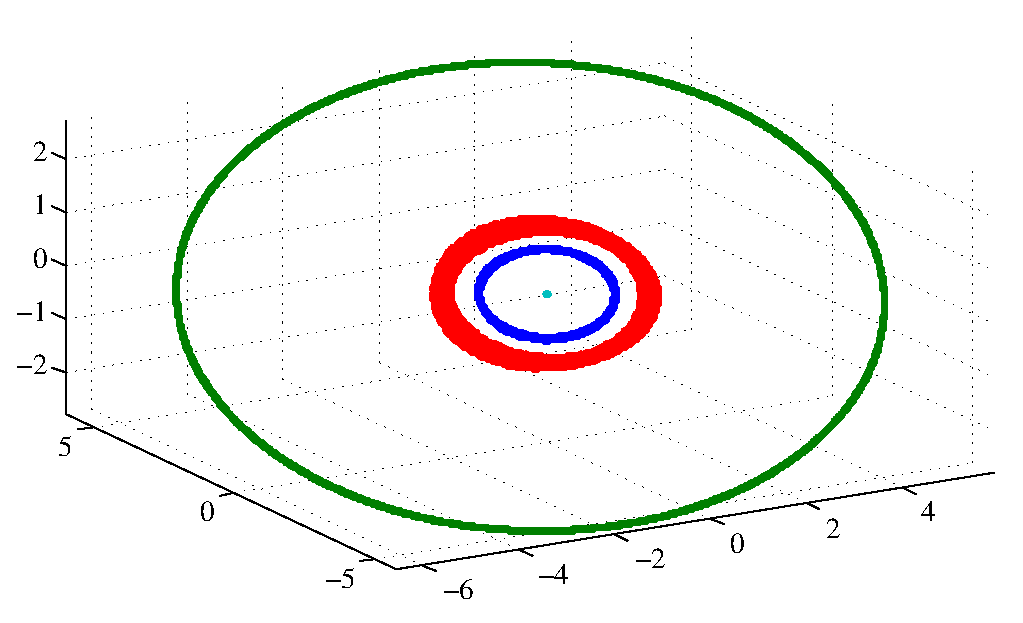
\includegraphics[width = 5.5in]{./figures/subSolSys}
  \caption[Sample Multi-body exosystem ]{ \label{fig:subSolSys} Orbits over 1 million years for exosystem composed of analogues of Earth (blue), Mars (red) and Jupiter (green), with a 1.5 $L_\odot$ star and orbits scaled such that all planets receive the same flux as they would in our solar system.  Note that over this time span, the Jupiter analogue causes significant deviations from the Keplerian approximation in the orbits of the two minor planets.  Scale units are in AU.}
\end{figure} 
While it is difficult to determine global stability of n-body systems, it is possible to determine local stability by integrating over long periods of time (millions of years) and searching for collisions or ejections (see \S\ref{sec:sysProp}).

The third approach to generating planetary systems represents the widest possible range of possible exosystems and is also the most difficult to apply.  One possibility is to `grow' solar systems by starting with simulated nebulae and utilizing a formation model to develop planets.  This is quite costly as it requires integrating many millions of years of the simulated system and often results in single-planet systems as bodies are ejected or destroyed.  An alternate method is to sample the known mass and semi-major axis distributions (see \reffig{fig:currHists}) and generate systems composed of multiple such bodies with initial conditions determined by Keplerian approximations.   However, using Keplerian approximations for initial conditions makes it difficult to simulate systems with non-Keplerian, n-body effects such as resonances \citep{fabrycky2010non} and long integrations are still required to ensure system stability.

The procedure for generating completely arbitrary planetary systems begins with the generation of $N$ random mass values according to the best-fit mass distribution.  From these masses the planetary radii are determined as follows:  For mass ranges up to 10$M_\oplus$, two random numbers are generated: a boolean value determining whether the planet will be a rock/iron or rock/ice mixture, and a random number uniformly distributed $\in [0,1]$, determining the fraction of rock via \refeq{eq:rockyPlanDensities}.  For giant planets, a uniformly distributed random number is generated in the range of [0,1] to represent the portion of mass in the planet's core, and radii values are interpolated from a lookup table based on values in \citet{fortney2007}.
 
Each planet is then associated with one of the target stars, with the likelihood of association given by the overall occurrence rate of planets and the iron abundance of the stars in the target list. Each planet is assigned an average albedo value ($p$) drawn from a uniform distribution in the range [$p_{min}$, $p_{max}$].  There is currently much work being done to model albedo values as functions of other planetary properties, but no one model is able to capture the entire parameter space \citep{sudarsky2005}.  For each planet, we generate initial positions and velocities by generating randomized average orbital elements via the distributions in \S\ref{sec:analytic_dists}. The mass of each target star is calculated from its absolute V magnitude ( $M_V$) via the relation:
\begin{equation}\label{eq:lmr}
\log(m_S/m_\odot) = 0.002456M_V^2 - 0.09711M_V + 0.4365 \,.
\end{equation}
 This relation has been shown empirically to be accurate to within 7\% for mass ranges corresponding to visual magnitudes between 1.45 and 10.25 \citep{henry1993}.  We treat the output of \refeq{eq:lmr} as the `estimated' mass and generate a `true' stellar mass as
\begin{equation}
m_S^{est} = m_S^{true}(1+ \nu)
\end{equation}
where $\nu$ is a random error term consistent with the known accuracy of \refeq{eq:lmr}.  The true masses are used for propagating the planets along their orbits, while the estimated masses of stars are needed for our return strategies, as described in \S\ref{sec:scheduling}.  This relation is used since it conveniently covers the range of visual magnitudes and stellar masses considered here.  However, newer mass-luminosity relations exist, with better accuracy for different mass ranges, and can be substituted for \refeq{eq:lmr} \citep{reid2002}.

At the end of this process, we have a target list encoded as an array of $N$ parameter sets
\begin{equation}\label{eq:simParamSet}
\{\begin{matrix} m_S^{est} &m_S^{true} & p_i & m_{P_i} & R_i & \mf r_{P_i/G} &  {}^\mc I \mf v_{P_i/G}& \mf r_{S/G} &  {}^\mc I \mf v_{S/G} \end{matrix} \}
\end{equation}
with $i = 1 \ldots n$ for a system of $n$ planets.  This parameter set can now be propagated forward in time to test the system stability and to perform mission simulations.  The set of parameter sets describing a group of simulated target systems will be referred to as a `universe' throughout the remainder of the text.

\subsection{System Propagation}\label{sec:sysProp}
Propagation of planets along their orbits can be done either by using the Keplerian formulation (which is exact only for a single-planet system) or by numerically integrating the Newtonian (\refeq{eq:nbody}) or post-Newtonian (\refeq{eq:einstein_nbody}) equations of motion.  If using the Keplerian formulation, the location of the planet is determined by the (possibly osculating) Keplerian elements and the current anomaly.  For the simulations in \S\ref{sec:case_studies}, the Keplerian propagation described here is used only for single-planet systems.  All simulations with multiple-planet systems use the n-body numerical integration methods described below.

From Equations (\ref{eq:Mdef}) and (\ref{eq:Pdef}) we can write:
\begin{equation}
M = \sqrt{\frac{\mu_S + \mu_P}{a^3}}(t - t_p) \, ,
\end{equation}
thereby directly relating the mean anomaly to the current time.  As the Kepler equation (\ref{eq:EtoM}) is non-invertible in $E$, we must use numerical methods in order to find the eccentric anomaly from the mean anomaly.  The simplest approach is to use Newton-Raphson iteration:
\begin{equation}\label{eq:NewtonRaphson}
E_{n+1} = E_n - \frac{M - E_n + e\sin E_n}{e\cos E_n - 1} \, .
\end{equation}
This iterant is applied to some initial value $E_0$ until convergence:
\begin{equation}
E_{n+1} - E_n < \varepsilon
\end{equation}
where $\varepsilon$ is typically set to the machine precision value of the data type being used \citep{moler2004numerical}.  This method produces excellent convergence as long as $E_0$ is sufficiently close to the true value for $E$.  For most values of eccentricity, it suffices to use $M$ for $E_0$, but in highly eccentric orbits, the mean and eccentric anomalies will differ greatly throughout the orbit.  An alternate approach to selecting $E_0$ lies in examining the Taylor expansion of the Kepler equation:
\begin{equation}
M = E - e\sin E \approx (1 - e)E + \frac{e E^3}{6} + \mc O(E^4) \,.
\end{equation}
We note that for a fixed value of $e$ and for $\vert M - E\vert >> \varepsilon$, one of the first two terms of the expansion is much larger than the other.  We therefore select $E_0$ as:
\begin{equation}\label{eq:E0selection}
E_0 = \left\{  
   \begin{array}{l l}
    \frac{M}{1 - e} & \frac{M}{1 - e} < \sqrt{\frac{6-6e}{e}}\\
   \left( \frac{6 M}{e} \right)^{\frac{1}{3}}& \mathrm{else}
    \end{array}
    \right.
\end{equation}
Because the Newton-Raphson algorithm is iterative, it is impossible to make it more time efficient than the minimum number of iterations required to achieve the desired precision.  However, using the initialization algorithm described above, machine double precision can be achieved for any eccentricity (up to $1 - \varepsilon$) in under 30 iterations for arbitrarily sized arrays of Mean anomalies and eccentricities (see \refcode{code:invKepler}).

While \refeq{eq:NewtonRaphson} is guaranteed to result in the correct anomalies for closed orbits, it starts with orbital elements, meaning that if planetary positions are recorded using a position and velocity state, it would be necessary to first apply Equations  (\ref{eq:vec2orbelem1}) - (\ref{eq:vec2orbelemf}) in order to find the osculating orbital elements.  Then, an updated mean anomaly would be defined as:
\begin{equation}
M(t) = \left(M(t_0) + 2\pi\frac{\Delta t}{P_{orb}}\right) \,\mathrm{mod}\,\, 2\pi \,,
\end{equation}
where $\Delta t$ is the desired time interval of the propagation ($\Delta t = t - t_0$) and mod represents the modulo operator.  \refeq{eq:NewtonRaphson} would then be applied to find E(t), from which the updated position and velocity could be calculated via Equations (\ref{eq:rpsrot}), (\ref{eq:rpsP1}), and (\ref{eq:vpsP1}).

A more direct method, which efficiently combines the conversion and iteration and is applicable to all orbits (open or closed), is described by \citet{shepperd1985universal}, based on work by  \citet{goodyear1965completely,goodyear1966general}.  Following \citet{sundman1913memoire}, the solution to \refeq{eq:twoBody} can be written as a function of a single parameter $w$ where:
\begin{equation}
\frac{\mathrm{d} t}{\mathrm{d} w} = \Vert \mf r_{P/S} \Vert \,.
\end{equation}
This solution (sometimes referred to as the `f and g method') allows us to update positions and velocities from their initial conditions:
\begin{equation}
\mf r_0 = \mf r_{P/S}(t_0) \quad \textrm{and} \quad \mf v_0 =  {}^\mc I \mf v_{P/S} (t_0)
\end{equation}
by using the algorithm:
\begin{align}
\upsilon_0 &= \mf r_0 \cdot \mf v_0  \,,\\
\beta &= \frac{2\mu}{\Vert \mf r_0\Vert} - \mf v_0 \cdot \mf v_0  \,,\\
r &= \Vert \mf r_0 \Vert U_0 + \upsilon_0 U_1 + (\mu_S + \mu_P) U_2  \,,\\
t &= \Vert \mf r_0 \Vert U_1 + \upsilon_0 U_2 + (\mu_S + \mu_P) U_3 \label{eq:altKeplerEq}  \,, \\
\mf r(t) &= f \mf r_0 + g \mf v_0 \label{eq:fandg}  \,,\\
\mf v(t) &= F \mf  r_0 + G \mf v_0 \label{eq:FandG}  \,,
\end{align}
where $U_n$ are the universal functions $U_n(w,\beta)$ \citep{battin1987introduction} and
\begin{equation}
\begin{array}{l c l >{\hspace{2cm}} l c l}
f &=& 1 - \frac{(\mu_S + \mu_P) U_2}{\Vert \mf r_0 \Vert} & g &=& \Vert \mf r_0 \Vert U_1 + \upsilon_0 U_2 \\
F &=& \frac{(\mu_S + \mu_P) U_1}{r \Vert \mf r_0 \Vert} & G &=& 1 - \frac{(\mu_S + \mu_P) U_2}{r} \,.
\end{array}
\end{equation}
The $f$ and $g$ functions may be equivalently defined in terms of the Keplerian orbital elements as:
\begin{equation}
\begin{split}
f &= 1 - \frac{\Vert \mf r \Vert}{\ell} + \frac{\Vert \mf r \Vert}{\ell}\cos(\nu - \nu_0) \,, \\
g &= \frac{\Vert \mf r \Vert \Vert \mf r_0 \Vert}{\sqrt{(\mu_S + \mu_P) \ell}}\sin(\nu - \nu_0)  \,,\\
F &= \sqrt{\frac{\mu_S + \mu_P}{\ell}}\tan\frac{\nu - \nu_0}{2}\left(\frac{1 - \cos(\nu - \nu_0)}{\ell} - \frac{1}{\Vert \mf r_0\Vert} - \frac{1}{\Vert \mf r \Vert} \right) \,, \\
G &= 1 - \frac{\Vert \mf r_0\Vert}{\Vert \mf r\Vert}\left(1 - \cos(\nu - \nu_0)\right) \,,
\end{split}
\end{equation}
where $\nu_0$ is the true anomaly at time $t_0$.

Note that $\beta$ is proportional to the orbital energy and \refeq{eq:altKeplerEq} is a reformulation of Kepler's equation in terms of $w$, which itself can be related to the eccentric anomaly as:
\begin{equation}
w = \frac{E - E_0}{\sqrt{\beta}} \,,
\end{equation}
where $E_0$ is the eccentric anomaly at $t_0$.

The universal functions $U_n(w,\beta)$ may be defined implicitly as:
\begin{align}
U_0 &= \left\{ \begin{array}{l l}
\cos(w\sqrt{\beta}) & \beta > 0\\
\cosh(w \sqrt{-\beta}) & \beta < 0 
\end{array}\right. \nonumber \\
U_1 &= \left\{ \begin{array}{l l}
\sin(w\sqrt{\beta})/\sqrt{\beta} & \beta > 0\\
\sinh(w \sqrt{-\beta})/\sqrt{-\beta} & \beta < 0 
\end{array}\right.  \\
U_{n+2} &= \frac{w^n}{\beta n!} - \frac{U_n}{\beta} \nonumber \,.
\end{align}
Unfortunately, this definition is not amenable to numerical implementation as the computation of the various trigonometric functions invariably introduces errors and often leads to singularities as various terms ($\beta$ especially) tend to zero.  The equivalent series representation:
\begin{equation}
U_n(w,\beta) = \sum_{k=0}^\infty \frac{(-\beta)^k w^{n+2k}}{(n+2k)!} \,
\end{equation}
is more tractable, but may still have convergence issues in the general case.  \citet{shepperd1985universal} solves this problem by introducing a change of variable:
\begin{equation}
u = \frac{U_1(w/4,\beta)}{U_0(w/4,\beta)} \,
\end{equation}
which falls strictly in the range $u \in [-\vert \beta \vert^{-\frac{1}{2}}, \vert \beta \vert^{-\frac{1}{2}}]$.  Since the alternate formulation of Kepler's equation in \refeq{eq:altKeplerEq} requires only the first few universal functions, the problem may be greatly simplified by writing:
\begin{align}
U_0\left(\frac{w}{2}, \beta\right) &= 1 - 2q \,, \\
U_0(w,\beta) &= 2U_0^2\left(\frac{w}{2},\beta\right) \,,\\
U_1\left(\frac{w}{2},\beta\right) &= 2(1-q)u\,, 
\end{align}
\begin{align}
U_1(w,\beta) &= 2U_0\left(\frac{w}{2},\beta\right)U_1\left(\frac{w}{2},\beta\right) \,, \\
U_2(w,\beta) &= 2U_1^2\left(\frac{w}{2},\beta\right) \,,
\end{align}
where
\begin{equation}
q = \frac{\beta u^2}{1 + \beta u^2} \,.
\end{equation}
Furthermore, 
\begin{equation}
U_3(w,\beta) = \frac{4}{3} U_1^3\left(\frac{w}{2},\beta\right) G(3,0,\frac{3}{2},q) \,,
\end{equation}
where $G$ is the continued fraction expansion of the ratio of the ratio of two hypergeometric series:
\begin{equation}
G(a,b;c;z) = \frac{{}_2F_1(a,b+1;c+1;z)}{{}_2F_1(a,b;c;z)} \,,
\end{equation}
with the Gaussian hypergeometric function defined as in \refeq{eq:gaussHyper}.

Returning to Equations (\ref{eq:fandg}) and (\ref{eq:FandG}), we see that the position and velocity can be updated via a simple matrix multiplication:
\begin{equation}
\left[\begin{matrix} \mf r(t) \\ \mf v(t) \end{matrix} \right] = \left[\begin{matrix} f I_3 & g I_3 \\ F I_3 & G I_3\end{matrix} \right]\left[\begin{matrix} \mf r_0 \\  \mf v_0 \end{matrix} \right] \,,
\end{equation}
where $I_3$ represents the $3\times3$ identity matrix.  Multiple bodies can be updated together by making the state transition matrix block diagonal and stacking positions and velocities into a single column vector:
\begin{equation}\label{eq:stackedState}
\left[\begin{matrix} \mf r_1(t) \\ \mf v_1(t) \\ \vdots \\   \mf r_n(t) \\ \mf v_n(t)\end{matrix} \right] =
\left[\begin{matrix} 
\left[\begin{matrix}f_1 I_3 & g_1 I_3 \\ 
F_1 I_3 & G_1 I_3\end{matrix} \right] & &\\
&  \ddots &  \\
& &\left[\begin{matrix} f_n I_3 & g_n I_3   \\ 
F_n I_3 & G_n I_3 \end{matrix} \right]
\end{matrix} \right]\left[\begin{matrix}  \mf r_1(t_0) \\ \mf v_1(t_0) \\ \vdots \\   \mf r_n(t_0) \\ \mf v_n(t_0)\end{matrix} \right] \,.
\end{equation}

In this formulation, the Kepler equation is solved via Newton-Raphson iteration on the independent variable, $u$:
\begin{equation}
u_{n+1} = u_n - \frac{t - \Delta t}{4(1 - q) r} \,.
\end{equation}
A secondary iteration is required to evaluate the function $G$.  A convenient algorithm is Shepperd's modification of Gautschi's method for the evaluation of continued fractions.  To evaluate the function $G(a,b;c;z)$, a set of intermediate variables is initialized as:
\begin{align}
k_0 &= 1 - 2(a - b) \,,\\
l_0 &= 2(c-1) \,, \\
d_0 &= 4c(c-1) \,, \\
m_0 &= 4b(c-a) \,, \\
A_0 &= B_0 = G_0 = 1 \,,
\end{align} 
and then iterated until convergence via:
\begin{align}
k_{n+1} &= -k_n \,,\\
l_{n+1} &= l_n + 2 \,, \\
d_{n+1} &= d_n + 4l_{n+1} \,, \\
m_{n+1} &= m_n + (1+k_{n+1})l_{n+1} \,, 
\\
A_{n+1} &= \frac{d_{n+1}}{d_{n+1} - m_{n+1} A_n z} \,,\\
B_{n+1} &= (A_{n+1} - 1)B_n \,,\\
G_{n+1} &= G_n + B_{n+1} \,.
\end{align} 
An implementation of the full algorithm is shown in \refcode{code:keplerSTM}.

For multi-planet system, we abandon the Keplerian propagation in favor of numerical integration of \refeq{eq:nbody}.  While this is more computationally intensive, it produces much more accurate results in systems with multiple planets, especially when one or more of these is Jupiter-size or larger.  More importantly, the Keplerian formulation cannot be used to generate consistent stellar reflexes in multi-planet system and is therefore a poor model for studying precision astrometry and radial velocity.  Because the Keplerian formulation places the star at the  origin of a frame that is treated as inertial, the Keplerian formalism implies that the star does not move.  Using the standard definition for center of mass, $G$,:
\begin{equation}
\sum_{k\in X}m_k \mf r_k/G = 0 \,,
\end{equation}
where $X$ is the set of all of the bodies in the exosystem (see \refeq{eq:Xsetdef}), the position of the star with respect to the barycenter is:
\begin{equation}\label{eq:keplerCOM}
\mf r_{S/G} = -\frac{\sum_{k \in Y} m_k \mf r_{k/S}}{\sum_{j \in X} m_j} \,,
\end{equation}
where $Y$ is now the set of all exosystem bodies excluding the star, $Y = X\backslash \{S\}$.  
If we consider the Newtonian formulation of the two body problem, as in \refeq{eq:twoBody}, with 
\begin{equation}
\mf r_{P/S} = \mf r_{P/G} - \mf r_{S/G} \,,
\end{equation}
where $G$ is now the barycenter of the two-body system, we see that \refeq{eq:keplerCOM} is the average of the star position with respect to the barycenter of each of the two-body systems composed of the star and each individual planet.  This means that rather than modeling the true interactions of all of the bodies in the system, the best that can be accomplished via the Keplerian model is a first order approximation of the true stellar motions.

The specific method used for the numerical integration is very important.  Because an orbital system with no external perturbations is a canonical Hamiltonian system, it is important to ensure that energy is being conserved.  Low order Runge-Kutta methods will not do so, deviating quite quickly from the true system state.  The solution is to use either high order integrators, or one of a class  of symplectic integration schemes.  Of particular interest are the Runge-Kutta-Nystr\"{o}m (RKN) methods as they are specifically formulated to solve second order ODEs that are cyclic in the first derivative of the state:
\begin{equation}
\frac{d^2}{dt^2} y = f(y) \,.
\end{equation}
While these methods also do not guarantee that energy will be preserved, they are canonical, and sufficiently high-order implementations preserve energy to a very large degree \citep{qin1991}.  \reffig{fig:integratorComp} shows a comparison of energy variation over time in numerical integrations of the solar system.
\begin{figure}[ht]
 \center
 \includegraphics[width= 5.5in]{./figures/integratorComp}
  \caption[Integrator Comparison]{ \label{fig:integratorComp} Change in total energy (\refeq{eq:Etot} over 25 years of integration of the solar system using different numerical solvers with identical initial conditions.}
\end{figure} 
Unlike the two RKN implementations, the Adams-Bashforth-Moulton (ABM) PECE (prediction-evaluation-correction-evaluation) multi-step solver \citep{shampine1975computer} and Runge-Kutta-Fehlberg (RKF) 7(8) solver \citep{fehlberg1968classical}, operate on first order ODEs.  However, the high order of the Runge-Kutta-Fehlberg (RKF) makes it outperform the (relatively) lower-order Runge-Kutta-Nystr\"{o}m 8(6) solver \citep{papakostas2000,qin1991} in terms of energy conservation.  The overall best performance is achieved with the  Runge-Kutta-Nystr\"{o}m 12(10) solver \citep{dormand1987high}.  The ABM solver, while multistep, does not have volume or energy preserving qualities and is thus the poorest  choice.  Over relatively short periods (less than 1 million years), the 12/10th order RKN solver is energy-preserving to within machine double precision.  For most system energy is stable on the order of $10^{-12}\%$ over billions of years. 

It is also common to use hybrid-symplectic integrators which use symplectic integration schemes when masses interact closely, and non-symplectic schemes the rest of the time to greatly increase the speed of integration without losing the energy-conserving properties of fully symplectic integrators \citep{chambers1999hybrid}.  However, because of the amenability of the n-body equation to vectorization, and the constantly increasing speed of computer processors, very high-order methods such as the RKN 12(10) solver can be run with integration times of billions of years in feasible amounts of computer time by using variable time steps and efficient error estimation algorithms \citep{tsitouras1999cheap}.  \refeq{eq:nbody} can be evaluated very efficiently by precomputing four indexing arrays.  For a state vector $x$ representing $n$ bodies, with positions and velocities stacked in a column vector as in \refeq{eq:stackedState}, $[j]$ is a vector of $9n$ elements filled with indices from $1$ to $n$ each repeated $n-1$ times:
\begin{equation}
[j] = [1, 1, \ldots , 1, 2, 2, \ldots , 2, \ldots , n] \,.
\end{equation}
The vector $[k]$ also has $9n$ elements, but is filled by circularly permuting the indices such that $k \ne j$:
\begin{equation}
[j] = [2,3, \ldots , n, 1, 3, \ldots , n, 1, 2, 3,\ldots , n,\ldots ,1,\ldots ,n-1] \,.
\end{equation}
Finally, two indexing matrices are required: [z1] contains indices $1\ldots3n$, arranged in a matrix of dimension $3 \times n$ and [z2] contains indices $1\ldots n(n-1)$, arranged in a matrix of dimension $n \times n-1$.  In this way, every required combination of position differences can be computed as by indexing the state with $[z1]$ recursively indexed by $[j]$ and $[k]$ and \refeq{eq:nbody} can be evaluated by summing over the columns of the matrix resulting from indexing the difference combinations with $[z2]$.  An implementation of this algorithm is presented in \refcode{code:nbodyVect}.

Numerical integration also makes it simple to search for specific events, such as collisions (when $\Vert \mf r_{k/j} \Vert < R_k + R_j$) or ejections (when specific orbital energy changes sign).  The basic approach is to define a set of continuous functions that cross zero when an event of interest occurs and then to use root finding methods such as Regula-Falsi to pinpoint the exact time of the event when a sign change occurs in the function evaluation between integrator iterations \citep{press1992numerical}.  In this fashion the stability of generated exosystems can be evaluated by simply integrating for a period of one million years or more (depending on the time spans predicted by the planetary formation and evolution theories used).

\section{Target Selection and Availability}\label{sec:targ_selection}
A major factor in the planning and outcome of any planet-finding mission is the fact that we are limited to a very specific, non-isotropic population of possible target stars.  Each detection method has limitations on what stars can be used, and a specific preferred type of star, limiting which stars can be added to the target pool.  For example, for direct imaging of Earth-like planets, we need nearby stars so that we can observe large portions of their habitable zones.  We would also like to have low exo-zodi contributions, making older stars preferential, and would likely concentrate on F, G, and K stars similar to the sun.  On the other hand, if we were looking for self-luminous giant planets, we would preferentially target young systems with hot A and B stars.  Instrument characteristics and mission goals will always drive the initial pool of stars, but the final target list has an equally dramatic effect on the mission science returns.

For direct imaging, we always start with a list of all of the stars about which a planet from the planetary population of interest  could, at some point in its orbit, be observable by our instrument.  For example, if we are interested in Earth-twins in the habitable zone, we leave only those stars where a randomly oriented habitable zone orbit leaves the planet outside the instrument's projected IWA for a time longer than the required detection integration time for that star (as defined in \S\ref{sec:model_obs}).  In order to decide whether a given star can have detectable planets in a region of interest (defined by some range of $a$ and $e$), we need to find the smallest possible $\Delta$mag for a planet in this region that corresponds to a value of $s$ greater than the projected IWA.  This is done as follows:
\begin{enumerate}
\item Find $\beta^\star$ that minimizes $\Phi(\beta)\sin^2(\beta)$.
\item Define the range of orbital distances as $r = [a_{min}(1-e_{max}),a_{max}(1+e_{max})]$.
\item Define $s_{\beta^\star} = r\sin\beta^\star$ and $\hat{r} = \textrm{IWA}*d/\sqrt{L} \sin\beta^\star$ - the minimum $r$ such that $s_{\beta^\star} >  \textrm{IWA}*d/\sqrt{L} $.
\item If $\hat{r} \in r$ then $s =  \textrm{IWA}*d/\sqrt{L}$ and $\beta = \beta^\star$.
\item If $\hat{r} < r$ then $s = \min(r)$ and $\beta = \beta^\star$.
\item if $\hat{r} > r$ then $s =  \textrm{IWA}*d/\sqrt{L}$ and $\beta = \sin(\textrm{IWA}*d/\sqrt{L}/\max(r))$.
\end{enumerate}
The $s$ and $\beta$ values produced by this algorithm represent the minimum value of $\Delta$mag for any planet in the region of interest, with the corresponding $s$ value outside the projected IWA.  If this $\Delta$mag value falls below the limit of the instrument's photometric sensitivity, then the star is considered a candidate. 

Additional criteria for the target list may include:
\begin{itemize}
\item Stars on the main sequence
\item Stars with high life expectancy (B-V Johnson magnitude > 0.3)
\item No low metallicity stars (higher probability of planets, see \reffig{fig:marcyFEH} 
\item No stars with high intrinsic variability (to remove major photometric variations)
\item No binaries or stars with close companions or nearby bright background stars (since most starlight suppression systems cannot work on multiple sources)
\item Maximum apparent magnitude (brighter stars only)
\item No young stars (so that planets will have formed)
\end{itemize}
 Young stars may be identified by X-ray emission for stars more distant than 15 pc (detected by ROSAT) \citep{guillout1999stellar}, by chromospheric variability, by rotational periods of less than 10 days, or projected rotational velocity of greater than 5 km/s. For a typical imaging mission such as the ones in \S\ref{sec:case_studies}, we start with the 1612 non-binary stars within 30 pc of our solar system.  For an IWA of 75 mas and $\Delta$mag$_0$ of 26, applying the procedure above to the subset of main sequence stars yields 372 possible target stars.  With those instrument specifications, 144 of these targets have single-visit completeness values of less than 0.01, and 260 have completeness values of less than 0.1.

The biggest problem in selecting the target list comes from one of the inherent trade-offs in the stated science goals.  The desire to visit as many unique targets as possible means that the overall probability of detecting planets is decreased by including lower completeness stars (where the probability of detection is smaller).  On the other hand,  only visiting a small number of stars automatically limits the number of unique detections that can be made, and if the frequency of the planet type you are searching for (or absolute frequency of all planets) happens to be low, having a large target pool may be the only way to detect any planets at all.  An additional problem lies in trying to filter target stars by the amount of integration time required.  Although we can calculate the integration time for any assumed $\Delta$mag value, in reality, planets from any population of interest can vary by several magnitudes at the time of observation.  For example, an Earth-twin observed at one point on its (habitable zone) orbit at a $\Delta$mag of 26 will require 200 days for spectral characterization.  The same planet, at a different orbital position can have a $\Delta$mag of 25, which would require only 30 days of integration.  In both cases, the time required to determine whether a detection has occurred is less than 2 days.  Because of the great disparity in detection and characterization times, and since high ecliptic latitude stars have very long observing seasons, improper mission simulation logic can sometimes lead to extremely long integration times which adversely affect overall mission performance.

Because we cannot assume \emph{a priori} knowledge of  planet frequency, or what the brightness of planets will be at the moment of detection, it is quite difficult to address these issues using scheduling logic alone.  Instead, we can introduce two additional parameters: a minimum target system completeness value, and a maximum single integration time.  The minimum completeness gives us a systematic way to limit the size of target lists, mapping directly to the unique targets vs.~total detections tradeoff. The maximum integration time allows us to include all potential targets, but not allow any one integration to significantly affect the mission outcome.  This value can be used in two different ways: first, the target list is filtered so that no detection time for the worst case (highest zodi level and limiting $\Delta$mag) exceeds the minimum integration time.  Second, in visits where a detection occurs, but the spectral characterization would take more than the maximum integration time, the spectral characterization is not attempted. 

The proper value for each of these parameters is found by performing a line search over multiple simulations with these values smoothly varied to optimize specific target metrics.  For all of the instruments and mission scenarios evaluated to date, there is improvement in the number of total and unique detections when the minimum completeness is raised from zero.  Specific improvements vary between instrument and spacecraft designs, but all systems perform better with a minimum completeness of 0.1, as opposed to using the full target list.  In cases where low completeness stars (completeness  $< 0.1$) do provide detections, these are always very dim, require much longer integration times to acquire a spectrum, and are never detected again.  The integration time cutoff is harder to optimize due to the larger search space and the computational costs associated with running many simulations.  In certain cases, the instrument design itself leads to a systematic limit on the length of observations, thereby automatically providing a maximum integration time.  In other cases, good results were achieved by setting the maximum integration time based on the total observation time available and the average time to transfer between targets.

For ground based observatories, target availability is given strictly by the observatory location and the time of year.  Space telescopes, however, can reside in a variety of orbits, and target availability may differ greatly from one observation to the next.  Missions such as Kepler, whose target pool is always in the field of view do not have any scheduling considerations associated with target availability, so the discussion in this section is limited to direct imaging missions and hybrid missions with targeted transit photometry or other planet-finding observations.

In general, whether a target star is observable at a specific point in time can be determined by calculating the angle between the telescope-sun and telescope-target vectors:
\begin{equation}
\theta = \cos^{-1}\left(\hat{\mf r}_{S/sc} \cdot \hat{\mf r}_{S_0/sc}\right)
\end{equation}
where $S_0$ refers to our sun.  For any given telescope, the sun cannot be within some number of degrees of the line of sight ($\hat{\mf r}_{S/sc}$ - the spacecraft-target vector) or light from the sun would enter the telescope aperture.  For a  telescope with a completely unshielded primary, this value would be nearly 180$^\circ$.  However, most optical telescopes are designed with the primary enclosed within the spacecraft and many proposed designs (especially for direct imaging) have sun shields that further extend the permissible location of the sun.  With these additions, the sun exclusion (or `keep-out') zone can be as low as 45$^\circ$.

\begin{figure}[ht]
 \center
 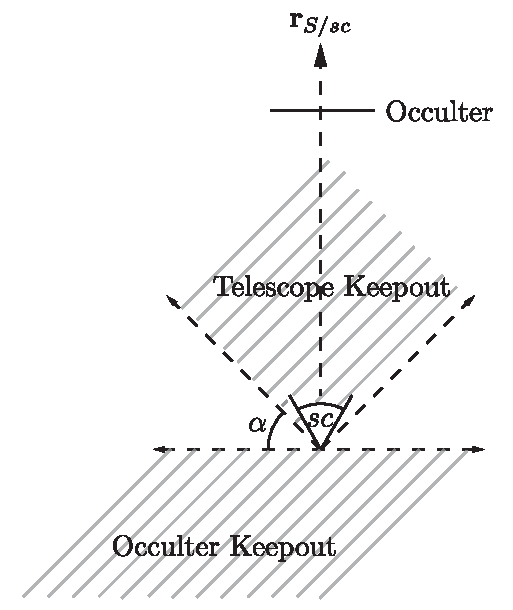
\includegraphics[width=2.75in]{./figures/keepoutZones}
  \caption[keep-out Zones]{ \label{fig:keep-outZones} Schematic top-view of telescope and occulter spacecraft and associated keep-out zones.  An observation can only be made when the sun (and any other sufficiently bright bodies such as the Earth or moon) is in the annulus extending $\alpha$ degrees (the complement to the sun-exclusion telescope angle) from the line orthogonal to $\mf r_{S/sc}$ at the telescope aperture.  If there is no external occulter, then the annulus also includes the 180$^\circ$ below this line.}
\end{figure} 

If the optical system is self contained, the sun exclusion angle is the only factor determining whether a star is in the keep-out zone.  Unfortunately, systems with external optical elements, such as free-flying occulters, have an additional keep-out zone so that sunlight isn't reflected by the external elements into the telescope.  Because of the nature of these systems, this keep-out region must cover the full 180$^\circ$ region below the line orthogonal to the line of sight (see \reffig{fig:keep-outZones}). It is possible to reduce this keep-out by tilting the occulter, at the expense of requiring larger starshades (as the effective shadow region is diminished) \citep{brown2010new}.


\section{Decision Modeling}\label{sec:scheduling}

While the assumptions and definitions in \S\ref{sec:model_obs} are sufficient to model any single observation with an imaging instrument, they are not enough to automatically generate an entire mission (or survey) timeline.  This is primarily due to the limitation of imaging systems to only one target at a time, and the strong stochastic element in the outcome of any one observation.  The amount of time spent on any one target will depend on whether an observable planet exists there, and also on how mission rules dictate that time be allocated to spectral characterization versus finding new planets.  Because the length of every observation is variable, the subset of available targets for the next observation (see \S\ref{sec:targ_selection}) will be constantly changing, and it is thus impossible to assemble an exact observation schedule before the start of operations.  For ground-based observatories, there is a natural cadence imposed by the day-night cycle, but it is still possible to optimize operations during a single night of observing, if real-time processing is employed.  Our goal is to develop a scheduling algorithm that will be able to make decisions based on the time history of previous observations.

Our automatic scheduler is defined as an optimization problem wherein we seek to maximize the science yield of a mission by simultaneously maximizing the number of unique planets discovered, the number of spectral characterizations of discovered planets, the number of planets observed enough times to produce orbital fits, and the portion of the target list observed at least once.  This last goal is included since there is scientific merit in any observation, whether or not a planet is detected (in the form of disk science and concurrent observations by other instruments on the observatory), and this provides a simple way of controlling the decision algorithm's natural bias towards higher completeness stars.  It must be noted that several of these science tasks are inherently antithetical---for example, spending time on finding more unique planets means less time devoted to scheduling additional observations for previously found planets, and thus fewer orbital fits.  This conflict is addressed by introducing weights to our cost function, which can be used to tune the relative importance of each science goal.

 Previous implementations of automated planning have modeled the order of observations as a traveling salesman problem (TSP) with repeated visits---a useful model as there exists a large body of work on methods for solving it \citep{kolemen2007}. Unfortunately, it is difficult to create a realistic mission simulation with this approach.  Unlike the classical TSP, where path lengths between locations are fixed and the group of locations remains invariant, here, the cost of transferring between a pair of target stars is time dependent, and the amount of time required at each target is variable, and cannot be known \emph{a priori}.  For these reasons, even the time-dependent TSP description of the system is inadequate.

Instead, as with a TSP, we represent the sequence of visits as a directed graph with variable length edges.  The graph is encoded as an $N \times N$ matrix (for $N$ targets), where element $ij$ represents the `cost' associated with switching from target $i$ to target $j$ (which we shall refer to as `transiting' between targets).  We can use a variety of graph search techniques to determine the optimum (least cost) path, by assuming that this matrix will remain constant for $k$ transits (where $k$ is determined by the specifics of the system being simulated), and thus pick the next target as the node generating the least cost path.  After a target is observed, however, the entire matrix is re-generated based on the current location of the spacecraft, and the process is repeated, thereby capturing the dynamic nature of the problem.  We can also take the approach of simply always going to the `best' (lowest cost) available target, by setting $k = 1$.  In cases where the matrix is relatively stable over multiple steps (i.e., the time spent on each target is small), the re-evaluation of the costs does not produce significant changes in the planned path.  However, in those cases where one observation takes a long time (i.e., when spectral characterization is required), the costs will change significantly, so it is very important to update the matrix to select the next best target.

The function determining the cost of each transit is a weighted linear combination of multiple factors,
\begin{equation}\label{eq:costfunc}
\begin{split}
A_{ij}  &= \left[ a_1 \frac{\cos^{-1}\left(u_i \cdot u_j\right)}{2\pi}B_{inst} + a_2 \textrm{comp}_j  \right. \\ 
&{} - a_3 e^{t_c-t_f} B_{unvisited} +  a_4 B_{visited}(1-B_{revisit})\\
&\left.{}  - a_5 B_{revisit} \left(\frac{N_j}{N_{req}} \right)(N_j < N_{req}) - a_6 \frac{\tau_j}{\textrm{vis}_j} \right] /(1-B_{keep-out}) \, .
\end{split}
\end{equation}
The first term represents the cost associated with retargeting, with $B_{inst}$ set equal to 0 for ground-based telescopes and space coronagraphs (since the amount of fuel and time used in retargeting should be approximately constant for an internal coronagraph for any pair of targets). $B_{inst}$ is set to 1 for space telescopes with external occulters, or any other system where a spacecraft needs to be physically repositioned in the line of sight from telescope to target.  While this term is not the actual cost associated with each specific retargeting (which depends on the position of the spacecraft and its orbit), it serves as a good heuristic function.  Because the orbits assumed for the telescope and occulter typically require active control to retarget in a reasonable amount of time, and the contribution of the orbital dynamics to the time and fuel costs of retargeting are comparatively small, in most cases this represents an admissible heuristic, and produces good results \citep{kolemen2007}. 

In calculating the actual transit time and fuel used, the full orbital dynamics and spacecraft masses are taken into account, and the masses are updated after each transit to reflect fuel use.  Following \citet{kolemen2008thesis}, transits are modeled either as impulsive thrusts or continuous point-to-point trajectories.  In each case, the aim is to find an occulter trajectory such that the telescope-occulter separation is fixed at the end, with inertial velocities matched. In the impulsive case, this is achieved with two large maneuvers at the beginning and end of the trajectory which are taken to change the occulter's velocity while keeping its position nearly constant.  This becomes a boundary value problem with the 3 dimensional velocity vectors at the trajectory endpoints as the unknowns, which can be solved via collocation.  

In the case where longer thrust times are required (such as with electric propulsion), the strategy is to minimize the control effort given the differential equations of motion and fixed endpoints (a fixed transfer time is assumed), which results in a 12 dimensional boundary value problem.  A detailed treatment of this problem type can be found in  \citet{stengel1994optimal} and the particular problem is analyzed in \citet{kolemen2007,kolemen2008thesis}.  Fuel use is calculated by assuming that the spacecraft mass is nearly constant during any impulsive thrust maneuver and taking the product of the burn time with the propulsion system mass flow rate, which is determined by the system  $I_{sp}\addsymbol{$I_{sp}$}{Specific Impulse}$ and thrust force.

The first term (when $B_{inst}$ is not zero) can be efficiently constructed by first generating a matrix of all of the combinations of the currently available target pool taken two at a time:
\begin{equation}
[c] = \left[ \binom{N_t}{2} \right] \,
\end{equation}
where $N_t$ is the size of the currently available target pool.  A vector of angular separations is calculated as in \refeq{eq:costfunc}:
\begin{equation}
[a] = \frac{\cos^{-1}\left(u_i \cdot u_j\right)}{2\pi}
\end{equation}
and then indexed via a strictly upper triangular (zero diagonal) matrix of ones to generate an upper triangular matrix of angular distances.  The result of this operation, when added to its transpose, generates the required matrix of the first term.  A sample implementation is presented in \refcode{code:genCostFunTerm1}.

For occulters designed to operate at multiple separation distances the slews required in order to complete spectral characterizations introduce high costs in terms of both fuel and time.  It is important to remember, however, that there is no effective way of minimizing these costs other than by changing the occulter design, so they need not be included in the transition cost function.  Since covering the whole spectral band is usually a mission requirement and observing seasons for most stars are relatively short, we have no choice but to move the occulter in at full thrust if characterizing the whole spectral band is to be attempted during a single visit.  Thus, the fuel/time cost of this extra slew is essentially constant (changing only gradually with the decreasing spacecraft mass) and does not affect the transition cost calculation any more than spectral characterizations performed by a coronagraph.  The only changes this system requires in the simulation logic are as follows: The occulter is moved for spectral characterization only if the star will remain observable for enough time to perform the slew and the second spectral integration.  In cases where the first half of the spectrum is acquired, but not the second, on revisits the occulter is slewed directly to the closer separation distance.  Because the smooth trajectories between the two separation positions do not take significantly different amounts of time or fuel, the heuristic term in the original cost function still applies.

The second term of the cost function serves as a heuristic for the probability of a detection at the next target, with  $\textrm{comp}_j$ equal to one minus the completeness of the $j$th target.  The third term is included to promote visits to as many unique targets as possible.  Here,  $t_c$ is the current time, $t_f$ is the mission lifetime, and $B_{unvisited}$ is a boolean equal to 1 if target $j$ has not been visited.  The fourth term creates a preference for targets that are scheduled for a revisit, with boolean $B_{visited}$  set to 1 if target $j$ has been visited, and boolean $B_{revisit}$ set to 1 if target $j$ is currently scheduled for a revisit (`currently', in this case, means $\pm$ the average re-targeting time).  The fifth term is included to improve the odds of good orbital fits.  $N_j$ is the number of previous detections of a planet at target $j$, and $N_{req}$ is the number of detections required for an orbital fit.  This term has the effect of biasing target selection towards those stars with more prior detections as they near the minimum required number of detections, when they are scheduled for revisits.  The inequality expression represents a boolean that eliminates the effect of this term once the required number of detections has been achieved.  

Nominally, we set $N_{req}$ to be four, but depending on the system and desired accuracy of derived orbital elements, many more detections may be required.  Since the method used to schedule future observations depends on an estimate of the semi-major axis, which is updated with each subsequent observation, we have found that four detections are generally enough to constrain the semi-major axes of planets in the limited population considered here to below 10\% error (in some cases to within 1\%).  Four visits also constrain the possible ranges of the other orbital parameters, giving us the ability to say with high confidence whether the planet is in the habitable zone.  Nevertheless, previous work has shown that orbital fitting accurate enough to predict the future positions of planets is very difficult, and may require many more observations, especially when considering more diverse populations of planets \citep{pravdo2007observation, brown2007minimumTPF}. 

The final term inside the brackets was included after a study of strategies employed in the manual scheduling of planet finding missions.  The most valuable of these strategies is to identify the stars closest to `leaving' a keep-out zone, and thus provide the maximum amount of possible integration time for the instrument.  This strategy has the additional benefit of creating a schedule in which an occulter does not need to move from target to target at full thrust (since slew times are determined by how much time is left until the star is viewable), thus saving large amounts of fuel.  This strategy is achieved by the sixth term, where $\tau_j$ is the amount of time before star $j$ enters a viewable zone (this value is negative if the star is already outside of the keep-out zone) and $\textrm{vis}_j$ is the total amount of time star $j$ is continuously viewable. This term has the effect of making stars about to enter a viewable portion of the sky more likely to be selected, while penalizing those that are about to enter a keep-out zone. 

The factors $a_i$ are selected to weight the relative importance of the various terms in \refeq{eq:costfunc}.  For the validation results presented in the next section, these terms were chosen manually, after experimenting with varying values.  Obviously, these weights represent a great opportunity for optimization and possibly auto-tuning during the course of a single simulation.  However, even with only six parameters, the search space of possible values is quite large, making an optimization remarkably computationally intensive.  The weights are also fairly specific to individual instrument designs, meaning that they cannot be carried over to new configurations unless these are fairly similar to previously analyzed ones.  Limited optimization, in the form of an unconstrained simplex search \citep{lagarias1999convergence} over a scalar cost function was carried out for the designs in \S\ref{sec:case_studies}.

Finally, $B_{keep-out}$ is a boolean representing whether a given star is currently in the keep-out zone.  Dividing by 1 minus this term leads to infinite costs for stars currently in the keep-out, so they are never selected; the same is done for the matrix diagonal so that the same target is not visited twice in a row.  For an occulter system, stars are only considered to be in the keep-out zone if they will be unobservable when the occulter completes its transition slew.  That is, if the amount of time until they become viewable would result in a transit slew using less than some selected factor of the slew time for thrusting (typically, we use 50\%), or if they could not be reached at full thrust before entering the keep-out zone.  Another way of controlling this is to define a default burn portion---that is, the default portion of the transfer maneuver that is used for accelerating and decelerating (with the remainder used for coasting).  This allows for an initial estimate of the slew times required to get to the next set of targets.  After the next target is selected, the actual burn portion used can be adjusted as necessary to achieve the desired transfer time.  Decreasing this parameter has the effect of saving fuel, as fuel use increases roughly as the square of the acceleration time, while potentially decreasing the number of targets visited. \reffig{fig:adjmat} shows a graphical representation of a cost function matrix.  In this case, all targets are included, leading to many whole columns of infinite values (for stars in the keep-out zone), however, to improve the efficiency of the simulation costs may be calculated only for the subset of stars not in the keep-out zone.
\begin{figure}[ht]
\centering
   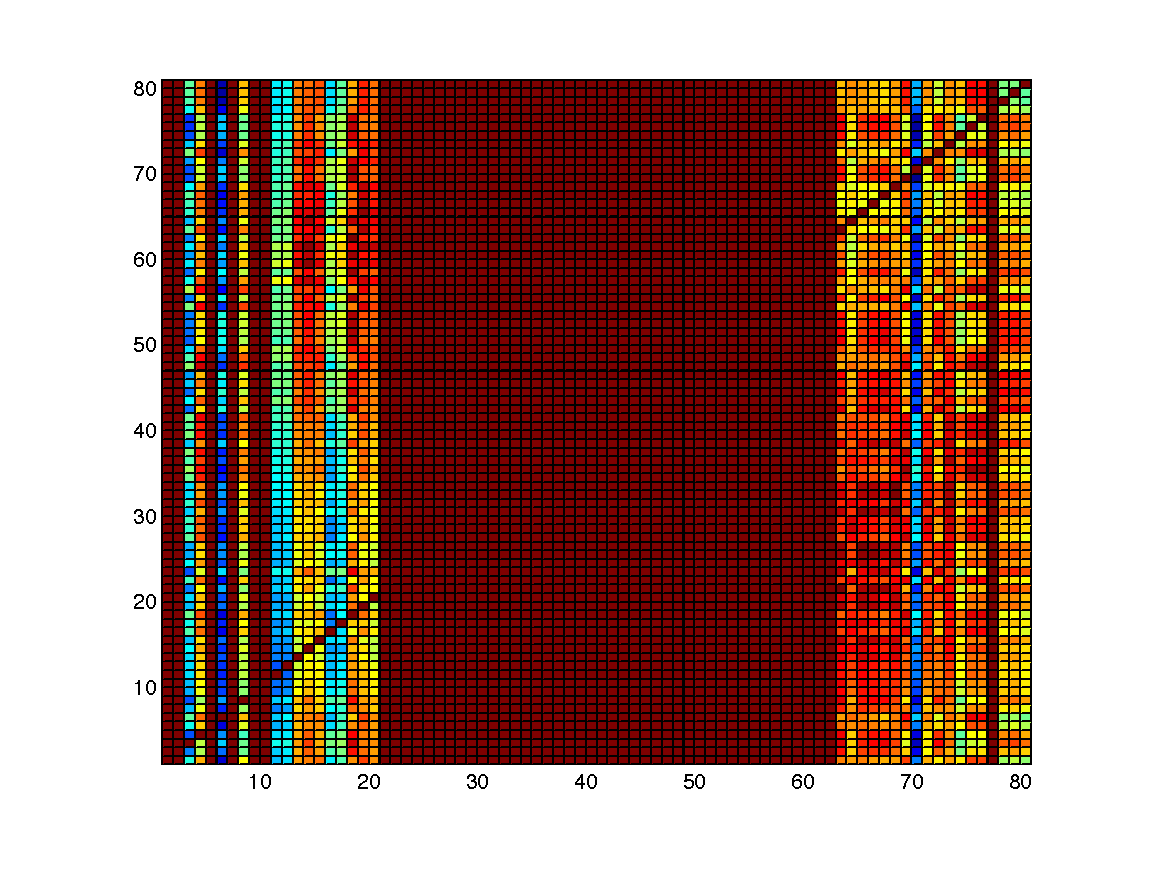
\includegraphics[width = 5.5in,clip=true,trim=0.5in 0.3in 0.5in 0.3in]{./figures/adjmatfig}
 \caption[Cost Function Matrix]{ \label{fig:adjmat} Visualization of cost function matrix.  All stars (including those in the keep-out zone) were included, leading to multiple columns of inifinite cost. The transition cost increases from blue to red.}
 \end{figure}

For the instruments considered in \S\ref{sec:case_studies}, those with an occulter will have transfer times between targets on the order of weeks, so that $k$ must be quite small---just two or three steps.  This makes it easy to compute all possible path costs and take the one representing the true minimum.  Self-contained coronagraphs, on the other hand, can acquire a new target in as little as a single day, while ground-based systems can retarget in just minutes, so that it is possible to use a much larger $k$, which would require switching to a different selection method (such as an iterative deepening search).  However, simulation shows that due to the relatively small target pools available, in most cases, just using the first 3 to 5 steps produces the same result as a more exhaustive search.  To minimize computing time fixed $k$ values of 3 are used for these instruments, except when directly testing the effects of varying this parameter.

The list of scheduled revisits (used to set the $B_{revisit}$ term in \refeq{eq:costfunc}) must be updated after every observation and is based on the outcome of the current observation (i.e., whether a detection occurs), the previous contents of the list, and the current time. As shown by \refeq{eq:aMLE}, if a detection occurs, the most likely estimate for the planet's semi-major axis is the observed apparent separation.  As shown in \refeq{eq:Pdef}, the orbital period (for a Keplerian orbit) is a function of the semi-major axis and the summed gravitational parameters of the star and planet.  If we assume that the mass of the star is much greater than the mass of the planet, then $m_S + m_P \approx m_S$.  The mass of the star can be approximated from its apparent magnitude via \refeq{eq:lmr}, and so we can estimate the orbital period from a single detection of the planet.

Because of the geometry of the system (see \reffig{fig:orbit_diagram} and (\ref{fig:imagingConstraintsSchem})), the best time to schedule a revisit (i.e., the most likely to result in a repeat detection) is either a full or half estimated orbital period after the initial detection.  If half of the estimated orbital period is used, this yields a higher probability that repeat detections will be on widely separated positions on the orbit, thereby improving the orbital fit.  If no detection occurs, we must rely on the mean orbital period of the planet population of interest, and schedule the return visit for 3/4 of this mean period.  Every subsequent detection can be used to improve our knowledge of the planet's orbital semi-major axis.  The probability density function of the ratio of $s/a$, calculated from \refeq{eq:aMLE} is used to  weight each recorded $s$ in order to update our estimate of $a$ \citep{savransky2007}.  \reffig{fig:revisitStrategies} shows the revisit detection rates when using these period estimates compared with a constant interval between observations.
\begin{figure}[ht]
\centering
   \includegraphics[width = 5.5in]{./figures/revisitStrategies}
 \caption[Revisit timing strategies]{ \label{fig:revisitStrategies} Comparison of revisit detection success rates using the estimated half orbital period, estimated full orbital period, and a constant value of one year, as a function of star absolute magnitude.  The simulated population is $a \in [0.4, 30]$, $e \in [0, 0.8]$, $p \in [0.1, 0.5]$, $R \in [0.7, 11.2]R_\oplus$, with orbits scaled so that planets receive the equivalent flux as they would for a 1$L_\odot$ star.  The constant interval case outperforms the period estimate case only in the case of the brightest stars, where planets are most often visible.}
 \end{figure}

It is important to point out that the return visit strategy may be significantly affected by the detection of multiple planets during the same visit.  If multiple planets are seen at wide angular separations during one observation, assuming that they have small mutual inclinations, it might be safe to assume that the exosystem was being viewed nearly pole-on, and thus would have already captured about as much of the habitable zone as possible, thereby negating the need for future visits if you were only interested in detection and spectral characterization (of course, multiple visits would still be needed for orbital characterizations).  Attempting to estimate the frequency at which multiple detections will occur during single observations is fairly difficult, since it depends completely on the makeup of exosystems.  Our currently small sample of multiple planet system contains a large fraction of `hot jupiters' due to the biases of the detection methods used.  These planets, due to their proximity to their primary stars, would not be detectable with the direct detection instruments studied here, and thus do not constitute a good test.  Instead, we can take our own solar system, and simulate randomly timed observations with the plane of the ecliptic randomly oriented with respect to the line of sight, and the system barycenter located a random distance from the observer.   Doing so for distances between 10 and 30 parsecs, with observations randomly placed in a 5 year window, and using a 75mas IWA instrument with a limiting $\Delta$mag of 26, produces slightly over 30\% of observations in which more than one planet could be seen, with only 4\% in which more than two are detectable.  

Furthermore, because Jupiter and Saturn are so highly detectable, the system orientation was classified close to pole-on (less than 10 degrees rotation) in only 20\% of these cases.  Thus, while it is probable that multiple detections will occur within single observations of systems structured somewhat like our own, this does not guarantee that we will be able to discount systems after a  single visit.  Even in cases where we will have good constraints on the exosystem inclination (i.e., when at least one of the planets detected is clearly in the inner system), one could argue that repeat observations as scheduled by the algorithm used here can be useful.  First, they will likely be required for confirmation---re-detecting a planet when it has moved noticeably on its orbit makes a much stronger case that the original detection was not of a background object or structure in the zodiacal dust. Second, while our solar system has very small mutual inclinations, we cannot discount the possibility that there exist stable exosystems with high mutual inclinations \citep{libert2007exoplanetary}.  

Another very important question that cannot be addressed with the single-planet system model is: in cases where a repeat observation of a target system where a planet has been previously discovered yields another detection, how can we determine whether we are seeing the same planet as before, or a new one?  This is often termed as `confusion' and can lead to significant inaccuracies in the gathered data set.  It is also  extremely important to rule out confusion when attempting to  confirm that initial detections really represent bodies that belong to the target star system, and to ensure that the data points we use for orbit fitting actually belong to the same data set.

One way to answer this question is to apply simple Bayesian theory.  The probability that a current observation is of the same planet as a previous one is given by
\begin{equation}\label{eq:bayesMultiPlanet}
P\left[\mathbf{p}_k | \mathbf{p}_{k-1},  \{\mathbf{p}_k,\mathbf{p}_{k-1}\} \in \mathbf{\gamma}_{k-1}\right] = \frac{P\left[\mathbf{p}_{k-1},\{\mathbf{p}_k,\mathbf{p}_{k-1}\} \in \mathbf{\gamma}_{k-1} | \mathbf{p}_{k}\right] P\left[(\mathbf{p}_k\right]}{P\left[\mathbf{p}_{k-1}\right]}
\end{equation}
where $\mathbf{p}_i$ is the parameter set recorded in the $i$th observation (i.e., star-planet separation and difference in magnitude), and $\mathbf{\gamma}_i$ is the space of all possible parameter sets belonging to a single planet that includes $\mathbf{p}_i$.  The likelihood, $p(\mathbf{p}_{k-1},\{\mathbf{p}_k,\mathbf{p}_{k-1}\} \in \mathbf{\gamma}_{k-1} | \mathbf{p}_{k})$, is approximately equivalent to the goodness-of-fit of a stable orbit to both data points, while the priors, $p(\mathbf{p}_k)$ and $p(\mathbf{p}_{k-1})$, can be calculated from the completeness distribution of the target star \citep{savransky2010occulting}.  This technique is demonstrated in \S\ref{sec:validation}.

\section{Simulation Methodology}
\refeq{eq:detIntTime} allows us to calculate how much time we need to spend integrating before we can assume, with a specific confidence, that no planet exists (or is currently observable by our instrument).  In the simulation framework, we calculate the required integration time for each target star assuming a planet observed at the IWA and the instrument's limiting $\Delta$mag.  For missed and null detections, this time value is used as the actual integration time (in a real mission, this would be the time spent integrating before moving on to the next target).  For detections, the integration time is recalculated based on the simulated planet's orbital position, using the actual separation (and throughput) and $\Delta$mag of the planet at the time of the observation (in a real mission, this would be the point when a detection could be confirmed via a bayesian technique and integration would either be stopped, or switched to spectral characterization).  False alarms (when no observable planet exists) and missed detections (when there is an observable planet) are generated at the rate determined by the FAP and MDP values used in calculating the integration time in \refeq{eq:detIntTime}.  Typically, the FAP and MDP are set to 1\% divided by the expected number of observations for the whole mission, and 0.1\%, respectively, which tends to yield zero missed detections and at most one or two false alarms per mission simulation for all of the cases considered in \S\ref{sec:case_studies}.

\begin{figure}[ht]
\centering
   \includegraphics[width = 6in]{./figures/simFlowchart}
 \caption[Simulation Flowchart]{ \label{fig:flowchart} Flowchart of simulation framework.  Ellipses represent optional steps determined by the specific instrument or rule set.}
 \end{figure}
\reffig{fig:flowchart} shows a flowchart for the full implementation of the simulation framework.  The basic steps of the simulation are as follows:
\begin{enumerate}
\item Generate single visit completeness values for all stars for the assumed planetary population. 
\item Generate target list based on given parameters and single visit completeness.  Assign planets to some subset of the target list based on selected planet frequency.
\item Generate the observatory orbit (including Earth rotation for ground-based instruments) and find all times over mission lifetime when targets will be observable.
\item Calculate maximum integration times for each target assuming planets at the IWA and $\Delta$mag$_0$, with the highest possible exo-zodi level.
\item Select initial target by choosing currently observable target with highest single visit completeness.
\item While the current time is less than the mission lifetime:
\begin{itemize}
\item Update visited list with current target.
\item If there is an occulter, calculate the disturbance forces acting on it at its present location.
\item If a planet exists in the target system, find its current angle on the sky and $\Delta$mag, the amount of  integration time required to detect it at the false alarm and missed detection probabilities being used.  If the planet will remain outside the IWA and be brighter than $\Delta$mag$_0$ for this amount of time, it is observable.  Otherwise, use the maximum integration time for this target, and increment the mission time by the integration time. If there is an occulter, decrement the spacecraft mass for stationkeeping for the integration.
\item If the planet is observable, generate a false negative (with probability of the missed detection rate) or a detection (with the complement probability 1).  If the planet is not observable, generate a false positive (with probability of the false positive rate) or a non-detection.
\item If a detection or false positive has occurred, and spectral characterization is called for, calculate the integration time required.  If the target star will be out of the keep-out for this amount of time, increment the mission time (and, if there is an occulter, decrement the spacecraft mass).  If the planet is observable for this whole time period, record a successful spectral characterization.  For coronagraphs, calculate and record the maximum observable wavelength.  If using a multiple distance occulter, attempt the second characterization in the same way.  
\item Add star and revisit time to the revisit list.
\item Calculate new cost function matrix based on current time and select next target.  If there is an occulter, calculate slew time and decrement spacecraft mass with the amount of fuel used.
\item If a portion of the mission is devoted to some other science, increment mission time by proportional amount.  Add spacecraft settling time before beginning next observation.
\item Propagate all of the planets in all target systems along their orbits by the total amount of time that has elapsed in this iteration step.
\end{itemize}
\end{enumerate}

At each step of this iteration, the state of the mission and all activities is encoded using the variables listed in Appendix \ref{app:DRMencoding}.  To check whether the final path generated is reasonable, and to allow for easier visualization of a whole mission timeline,  we can plot the sequence of observations on a map of the sky.  A sample of this is shown in Figure \ref{fig:theia_DRM}.  Because of the large number of inputs and parameters required to run a simulation, a graphical front-end was created to manage all of these.  \reffig{fig:DRMconstructor} shows the main panel of the application, called `DRMconstructor' used for setting up and running simulations. 
%
\begin{figure}[ht]
\centering
   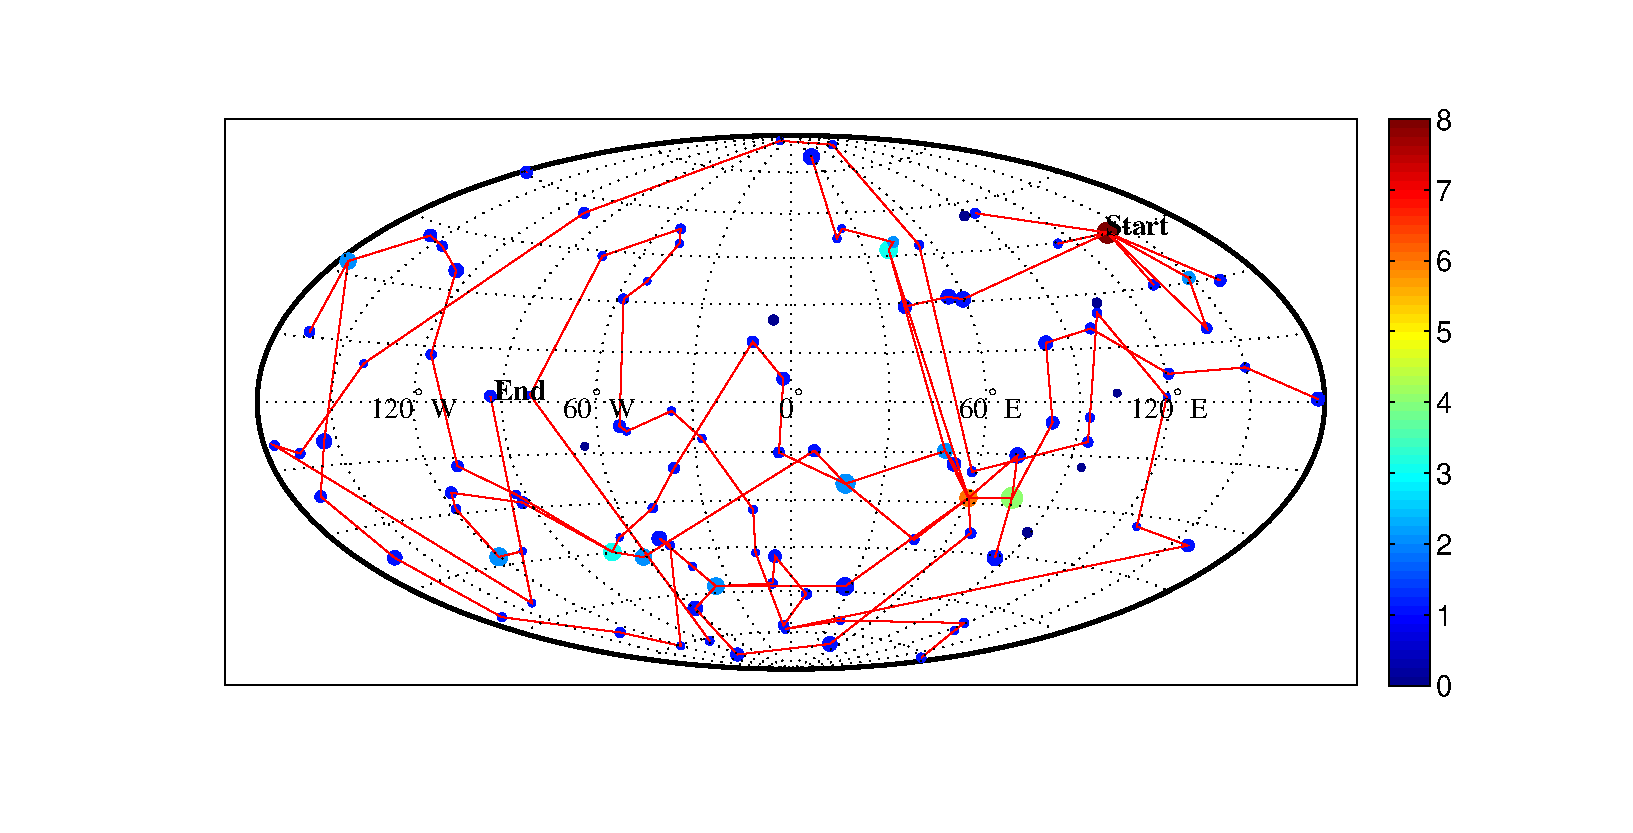
\includegraphics[width = 6in,clip=true,trim=1.2in 0.75in 0.9in 0.5in]{./figures/theia_DRM}
 \caption[Sample auto-generated DRM]{ \label{fig:theia_DRM} Visualization of an automatically generated sequence of observations. Points represent target stars, with size correlated with single visit completeness (i.e., the larger the point, the higher its single visit completeness). The color scale represents the number of observations made of a system in this simulation.  Note that some systems get many visits not because of their high completeness, but because they are well located on the sky.}
 \end{figure}
 \begin{figure}[ht]
\centering
   \includegraphics[width = 6in]{./figures/DRMconstructor}
 \caption[DRMconstructor]{ \label{fig:DRMconstructor} Graphical front-end of the DRMconstructor simulation utility.}
 \end{figure}

Because this process must be repeated many times in order to generate the ensembles of mission timelines required to calculate the distributions of various performance metrics, it is reasonable to attempt to parallelize as much of it as possible.  Fortunately, as each timeline can be evaluated independently of the others, generation of an ensemble is inherently parallelizable to an arbitrary number of processes by simply assigning each new simulation to the first available  process thread, or by pre-assigning an equal number of simulations to each thread.  The simulations in \S\ref{sec:case_studies} were all carried out on a multi-core, multi-processor machine, utilizing a maximum of 8 concurrent threads and a single local scheduler, but the basic framework can be easily extended to large distributed computing environments by substituting a remote scheduler.

\section{Case Studies}\label{sec:case_studies}

The purpose of this section is to demonstrate completed analyses of direct detection missions using the techniques described throughout this chapter.  Because one of the most important goals of planet-finding is the discovery of Earth-like planets, we use, as the base case, populations of Earth-twins.  Unless otherwise noted, the simulated systems in this section are populated with Earth-twins distributed throughout their habitable zones (defined as $a \in [0.7, 1.5]\sqrt{L}$ and $e < 0.35$) with either zero or one planets per system.  The term `Earth-twin' indicates planets of the radius and mass of the Earth, with a constant albedo of 0.22 (this value was selected to conform with previous studies, including \citet{lindler2007}) with isotropically distributed orbital orientations.  Exo-zodi levels are taken to be constant, with $\mu = 1.55$ to correspond to the historical average zodi brightness \citep{kuchner2008}.  When spectral characterization is possible, default mission rules call for one complete spectrum to be collected for each unique planet (meaning that spectral characterization is not performed during revisits unless a full spectrum was not taken at the initial detection, or the mission rules are modified). The settling time (i.e., the time to acquire a new target and begin observing) for all spacecraft is taken to be 24 hours. A full listing of the default parameters is available in Appendix \ref{app:defSets}.

All of the spacecraft are assumed to reside on a halo orbit about the Earth-sun L2 point.  For occulter systems (except in the case of O$_3$, see below) the telescope is placed on the halo orbit, which is assumed to be stable enough that only minor thrust corrections are required to keep the spacecraft on the orbit over the life of the mission.  The orbit of the occulter spacecraft, however, must be actively adjusted throughout the course of the mission, both to reposition the spacecraft for observing new targets (slewing), and to maintain precise alignment between the two spacecraft (stationkeeping).  The methods for generating stable halo orbits, as well as techniques for optimal point-to-point transfers about these orbits are developed in \citet{kolemen2008thesis}.  An example of the nominal halo orbit (510000 km in the azimuthal direction) is shown in \reffig{fig:halo_orbit}.
\begin{figure}[ht]
\centering
   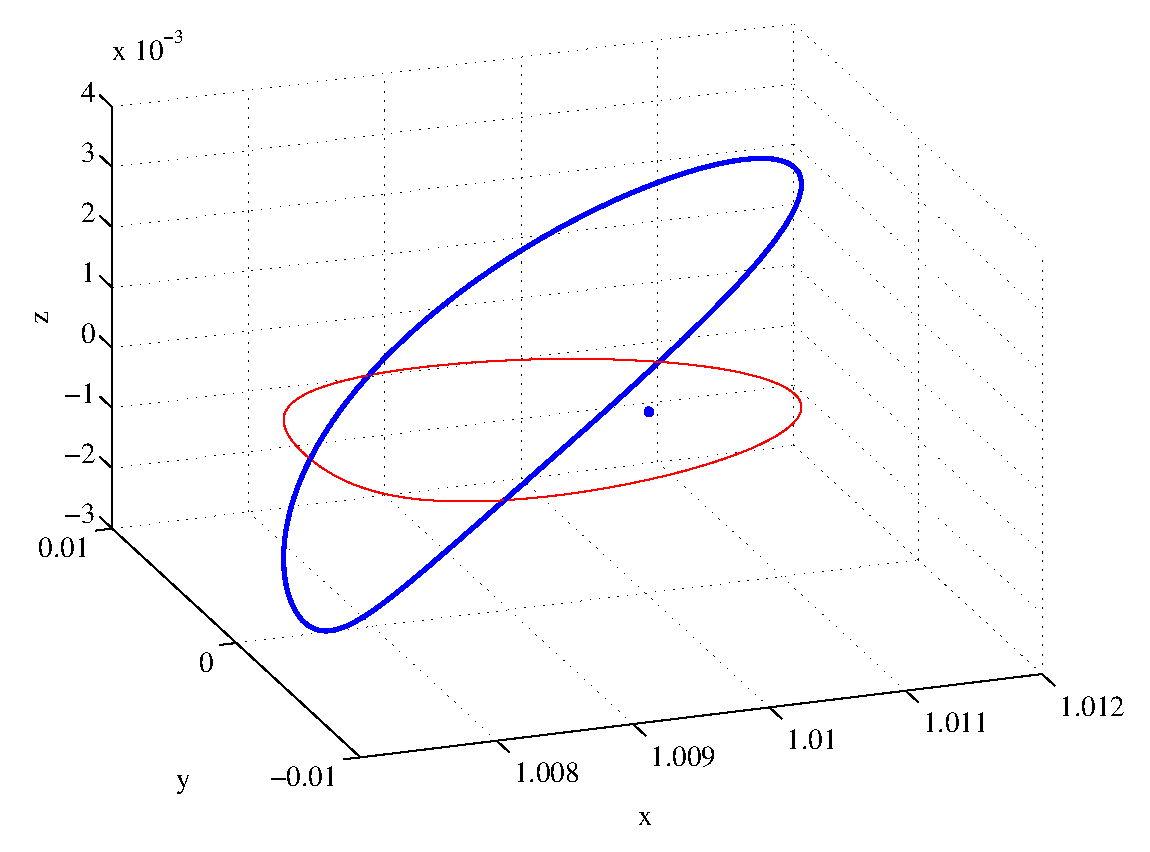
\includegraphics[width = 5.5in]{./figures/halo_orbit}
 \caption[Halo orbit]{ \label{fig:halo_orbit} Nominal halo orbit (510000 km azimuthal radius).  The blue point is the Earth-sun L2 point, while the red curve is projection of the orbit into the plane of the ecliptic.  Note that the out of plane component of the orbit is much smaller than the in-plane components.  Units are AU and the coordinate system is heliocentric, with $z$ perpendicular to the ecliptic, and $x$ increasing away from the sun}
 \end{figure}

Among the instruments and missions considered, some represent specific mission concepts that are relatively well developed (with a large number of design details and requirements available for the simulation), whereas some represent more generalized missions intended for high-level comparisons of different instrument types.  The various concepts are listed below, along with the basic parameters used to describe each.  Specific settings that were varied for certain instruments for particular tests or to maximize different metrics are detailed along with the simulation results in the following sections.
\begin{enumerate}
\item Generalized Single-Distance Occulter (SDO$\addsymbol{SDO}{Single-Distance Occulter}$) - The baseline occulter mission consisting of a circular aperture telescope and an occulter spacecraft operating at one separation distance from the telescope.  This type of occulter is designed to provide high contrast across the entire spectral band and is therefore larger than occulters designed to provide equivalent contrast over smaller bands \citep{cady2010design}.  Different propulsion systems may be employed for different designs (especially at differing telescope scales), but the baseline uses the same propulsion system as THEIA (see below).  Multiple designs have been created for telescopes of various aperture sizes, and are detailed in \reftable{table:occulters}.  
\item Generalized Multiple-Distance Occulter (MDO$\addsymbol{MDO}{Multiple-Distance Occulter}$) - Essentially equivalent to the generalized SDO, the MDO is designed to achieve high contrast over two (roughly) equal bands at different distances.  The majority of these designs use a second separation distance equal to half of the original, thereby operating at double the IWA for higher wavelengths.  See \reftable{table:occulters} for details.
\item Generalized Coronagraph - The baseline design for self-contained coronagraphs.  While not specifically modeling any one coronagraph type, this represents any of a number of high-throughput, low-IWA coronagraphs currently under development \citep{guyon2006theoretical,groff2010progress}.  Typical IWAs are either 2 or 3 $\lambda/D$, which corresponds to between 26 and 103 mas for a 4 m telescope---comparable to the geometric IWA of the baseline occulter for a 4 m aperture and detections in the V band.  By default, the coronagraph missions devote 50\% of their time to planet-finding activities (as opposed to coronagraphs, which typically use less than 33\%).
\item Telescope for Habitable Exoplanets and Interstellar/Intergalactic Astronomy (THEIA) Exoplanet Characterizer (XPC) \citep{spergel2009} - An MDO for a  4 m telescope developed as a flagship mission class concept study whose primary goal is the detection and spectral characterization of Earth-like planets.  The mission design yields high-contrast spectral capability over the 250 - 1000 nm band, split into two sub-bands, with geometric IWAs of 75 and 118 mas, respectively.  This allows for the detection of molecular oxygen at high confidence levels.  The mission rules developed to address the primary mission goal call for attempting to maximize the number of unique detections while heavily biasing the scheduling towards multiple revisits to a small candidate sub-pool of good targets (ones with previously discovered bright planets) to ensure at least a few orbit fits. A full spectrum (to resolution of R=70 at 760 nm) is also required for each unique detection.  The THEIA occulter uses paired NEXT ion thrusters \citep{patterson2002next} to provide up to 450 mN of thrust at a specific impulse of 4160 s.  Stationkeeping is performed with hydrazine thrusters with $I_{sp} = 220$ s.  The separate stationkeeping system was added due to concerns that the plumes produced by the electric propulsion system would be bright enough to interfere with observations.
\item Occulting Ozone Observatory (O$_3$) - An SDO or MDO for a 1.1 - 2 m telescope developed as part of a mission concept study aimed at finding a less expensive (\midtilde\$1 billion) planet-finder.  While O$_3$ can cover the same band as THEIA, the smaller aperture makes high resolution spectroscopy unreasonable, so O$_3$ focuses on band photometry, while retaining the ability to detect ozone, another biomarker \citep{heap2010detecting}.  When operating as an SDO, O$_3$ does not have photometric sensitivity beyond 550nm.  As an MDO, O$_3$ can operate in the `blue' band (250 - 550 nm) or the `red' band (500 - 1100 nm).  See \reftable{tbl:O3filters} for details on the photometric bands \citep{savransky2010occulting}.  Unlike the other occulters, O$_3$'s occulter spacecraft remains in an unperturbed orbit while the telescope spacecraft is repositioned between observations, using chemical thrusters providing a thrust of 500 mN at an $I_{sp}$ of 600 s.
\end{enumerate} 

\begin{table}[ht]
\caption{Occulter Designs. \label{table:occulters}}
\begin{center}
\begin{tabular}{ c c c c c }
\hline\hline
Telescope & Occulter &  50\% Throughput & Starshade & Petal\\
 Diameter  (m) & Type &  IWA (mas) & Mass (kg) & Length (m)\\
\hline
2 & SDO/MDO\tnote{\textasteriskcentered} & 69.6 & 2300 & 7\\
\hline
\multirow{2}{*}{4} & SDO  & 59 & 4200 & 19\\
			       &  MDO\tnote{\textdaggerdbl} & 57.5 & 3370 & 10\\
			       \hline
\multirow{2}{*}{8} & SDO & 56 & 7180 & 24\\
			       &  MDO  & 53 & 4915 & 13.5\\
			       \hline
16m & MDO & 47 & 10022 & 21.5\\		       
\hline
\end{tabular}

\medskip

\begin{threeparttable}[b]
\begin{tabular}{ c c c c }
\hline\hline
Telescope & Occulter & Starshade & Separation\\
 Diameter  (m) & Type &  Radius (m) & Distance (km)\tnote{\textdagger} \\
\hline
2 & SDO/MDO\tnote{\textasteriskcentered} & 17 & 38960/19480 \\
\hline
\multirow{2}{*}{4} & SDO & 25.6 & 70400 \\
			       &  MDO\tnote{\textdaggerdbl} & 20 & 55000/35000 \\
			       \hline
\multirow{2}{*}{8} & SDO & 35.2 & 96800\\
			       &  MDO & 27.2 & 74800/52360 \\
			       \hline
16m & MDO & 43.2 & 118800/83160 \\		       
\hline
\end{tabular}
\begin{tablenotes}
  \item [\textdagger] For MDOs, the first separation distance is used for covering 250-700nm, and the second for 700-1000 nm, except for O$_3$, which is split into the `blue' and `red' bands in \reftable{tbl:O3filters}.
    \item [\textasteriskcentered] This is the 1.5 - 2 m $O_3$ design.
    \item [\textdaggerdbl] This is the final design for THEIA.  The same design can also be used with a 1 m telescope.
   \end{tablenotes}
 \end{threeparttable}
 
 \end{center}
\end{table}

\begin{table}[ht]
\caption{O$_3$ filters. \label{tbl:O3filters}}
\begin{center}
\begin{threeparttable}[b]
\begin{tabular*}{0.8\textwidth}{@{}@{\extracolsep{\fill}} c c c @{}}
\hline\hline
\multirow{2}{*}{Filter \#} & \multicolumn{2}{c}{Bandpass ($\mu$)} \\
  & Blue & Red\\
\hline
1 & 0.25 - 0.31 & 0.5 - 0.7 \\
2 & 0.31 - 0.4 & 0.7 - 0.9 \\
3 & 0.4 - 0.48 & 0.9 - 1.1 \\
4 & 0.48 - 0.55 & Narrowband\tnote{\textdagger} \\      
\hline
\end{tabular*}
\begin{tablenotes}
    \item [\textdagger] The specific narrowband filter selection will be informed by results from transit photometry, which should help pinpoint the most interesting and common giant planet near-IR features, but will most likely coincide with a methane absorption feature.
   \end{tablenotes}
 \end{threeparttable}
 \end{center}
\end{table}

The point spread functions for the optical systems of these instruments are generated using different algorithms. Throughput curves for coronagraphs are created by sequentially generating tilted wavefronts at the telescope aperture and applying propagation algorithms to these.  For occulters, we use the Bessel expansion described in \citet{vanderbei2007} via a fast algorithm to calculate the electric field at the aperture of the telescope, assuming an incident plane wave on the occulter.  The field at the telescope aperture following a tilted incident wave may be related to the field from an incident plane wave by:
\begin{equation}
    E_{\mathrm{tilt}}(x, y) = e^{-i k \sin{\alpha} x} e^{i k z \cos{\alpha}} E(x + \sin{\alpha} z, y)
\end{equation}
which holds for small angles and allows the Bessel expansion for plane waves to be used. This field may then be fed into the appropriate propagation scheme.  (Propagation through the telescope with no coronagraph is treated as just a Fourier transform.)  In general, we prefer to examine throughput in terms of total energy in pupil planes rather than image planes, as the finite extent of the pupil planes ensures a more accurate measure of energy \citep{kasdin2006}.  It is important to note that the throughput curves shown in \reffig{fig:throughputs} are idealized, and achieving these levels of performance will require meeting exacting manufacturing and positioning tolerances for the occulters, and very precise wavefront control for the coronagraphs.
 \begin{figure}[ht!]
 \centering
 \subfigure[SDO Throughput]{ \includegraphics[width = 2.8in,clip=true,trim=0.25in 0in 0.25in 0in]{./figures/sdocculter_throughput}  \label{fig:sdocculter_throughput} }
 \subfigure[THEIA throughput]{\includegraphics[width =  2.8in,clip=true,trim=0.25in 0in 0.25in 0in]{./figures/theia_throughput} \label{fig:theia_throughput}}\\
 \subfigure[O$_3$ throughput]{ 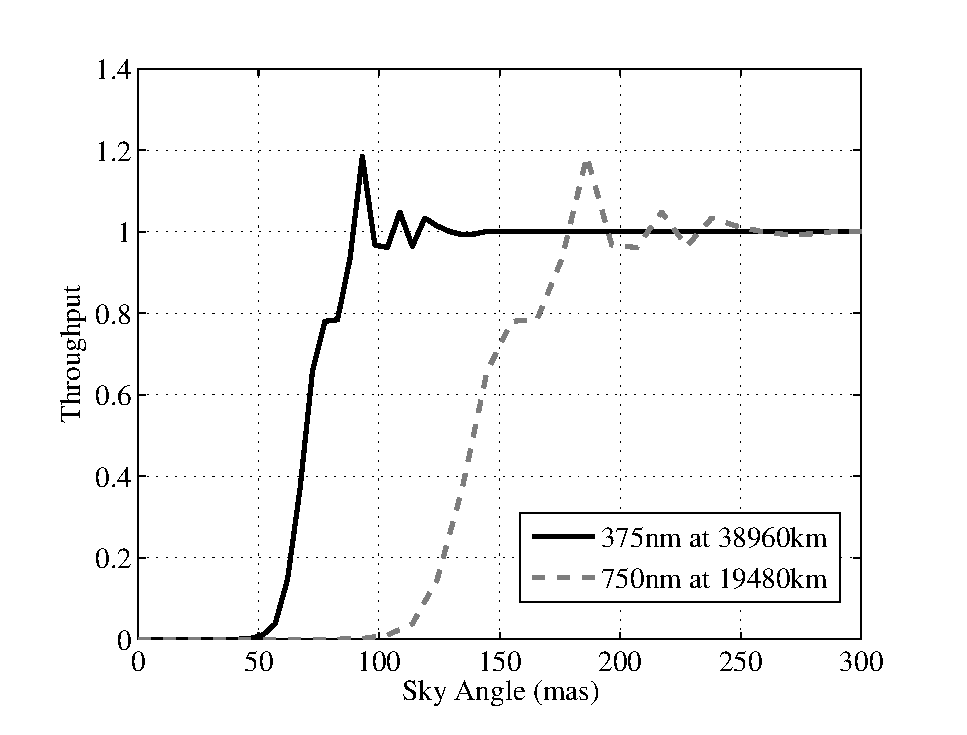
\includegraphics[width= 2.8in,clip=true,trim=0.25in 0in 0.25in 0in]{./figures/O3_throughput}  \label{fig:O3_throughput} }
 \subfigure[Coronagraph Throughput]{\includegraphics[width =  2.8in,clip=true,trim=0.25in 0in 0.25in 0in]{./figures/coron_throughput} \label{fig:coron_throughput}}
 \caption[Throughput Curves]{\label{fig:throughputs} Throughputs as functions of angle on the sky (units of mas for occulters occulters and $\lambda/D$ for coronagraphs). The throughput may be greater than unity for occulters since at certain angular separations, the occulter petals will send planet light into the telescope aperture that would otherwise have bypassed it. Data for (d) was provided by L. Pueyo (Personal Communication, 2009).}
\end{figure}

\subsection{Validation}\label{sec:validation}
Before we can use the results from mission simulations based on the decision modeling described in \S\ref{sec:scheduling}, it is necessary to determine whether the cost function described by \refeq{eq:costfunc}  actually produces optimal (or close to optimal) results.  Of course, the definition of optimality in this case depends entirely on what we want the mission to achieve, and how we prioritize the various science deliverables (i.e., how we set the weight factors $a_i$ in the cost function).  Still, if the cost function operates as designed, and all weights are set to be equal, we would expect the resulting simulations to maximize science yield while minimizing operational cost.  Since there is a direct tradeoff between time spent on new detections and time spent on characterizations, and between fuel use and available observation time, we do not expect a globally optimal solution for any of these.  Instead, we want to always be able to find the easily detectable planets in every universe, and to get orbits and spectra for as many of these as time permits, while reducing fuel use in designs with occulters.  

To test whether the framework described here accomplishes this, we can generate a `ground truth' case in the form of the distribution of all possible mission scenarios with a fixed set of target systems.  To do so, we generate one single universe, and compare the results of the mission simulation for this universe using our automated decision modeling to mission simulations with randomly generated visit orders.  Specifically, rather than using our decision modeling algorithm to decide on the next target, we simply select one at random from the list of targets currently outside of the keep-out zones.  By running this randomized visit order mission on the same universe multiple times, we can map the space of possible observing sequences and find a distribution of mission results.  We can also use a modified version of our framework that always selects the next available highest completeness target, rather than using the cost function in \refeq{eq:costfunc}.

\reffig{fig:optim_hists} shows the resulting histograms for the number of unique planet detections and successful spectral characterizations found from running 1000 randomized visit order missions on a single universe with $\eta_\oplus = 0.5$, using the THEIA and 2$\lambda/D$ coronagraph mission concepts.  On top of these, we have the results of the missions produced by the decision modeling algorithm with a depth of search ($k$) of either 3 or 1, and the results of the mission which only considers completeness in selecting visit order.  
For THEIA, using a $k$ of 3 and 1 produces the same values for both these metrics, whereas the $k=3$ case outperforms the $k=1$ case in terms of unique detections for the coronagraph. All cases using the scheduling algorithm described in \S\ref{sec:scheduling} outperform schedules based on just completeness.
\begin{figure}[ht!]
\centering
2 $\lambda/D$ Coronagraph\\
 \includegraphics[width = 2.8in,clip=true,trim=0.4in 0in 0.5in 0in]{./figures/optimhistsa}
 \includegraphics[width = 2.8in,clip=true,trim=0.4in 0in 0.5in 0in]{./figures/optimhistsb}\\
 THEIA\\
  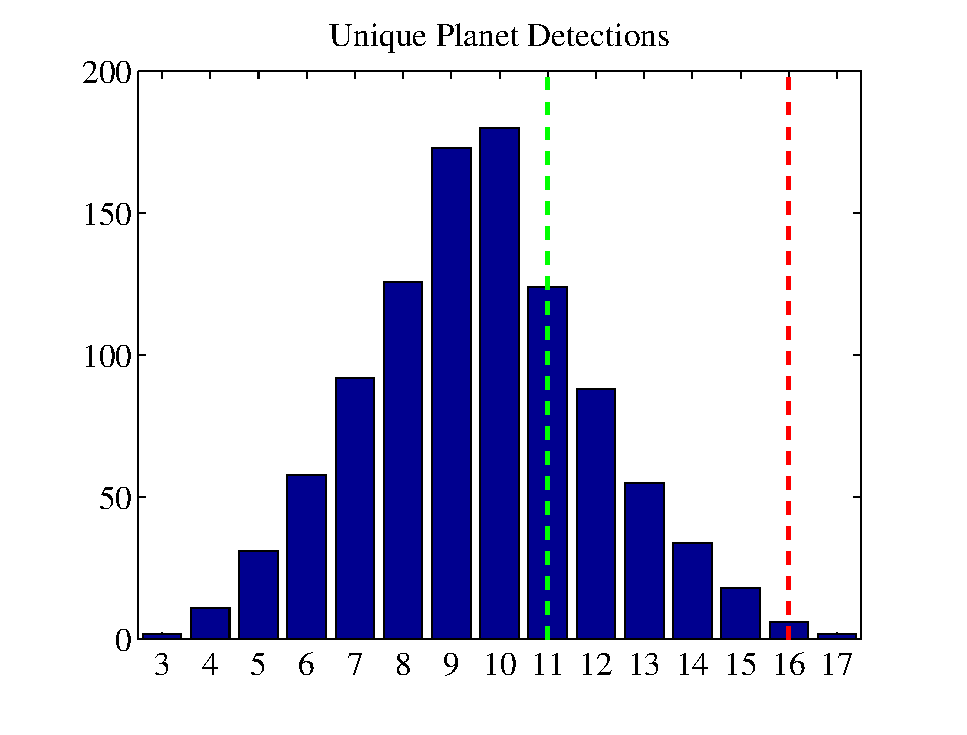
\includegraphics[width = 2.8in,clip=true,trim=0.4in 0in 0.5in 0in]{./figures/optimhistsc}
   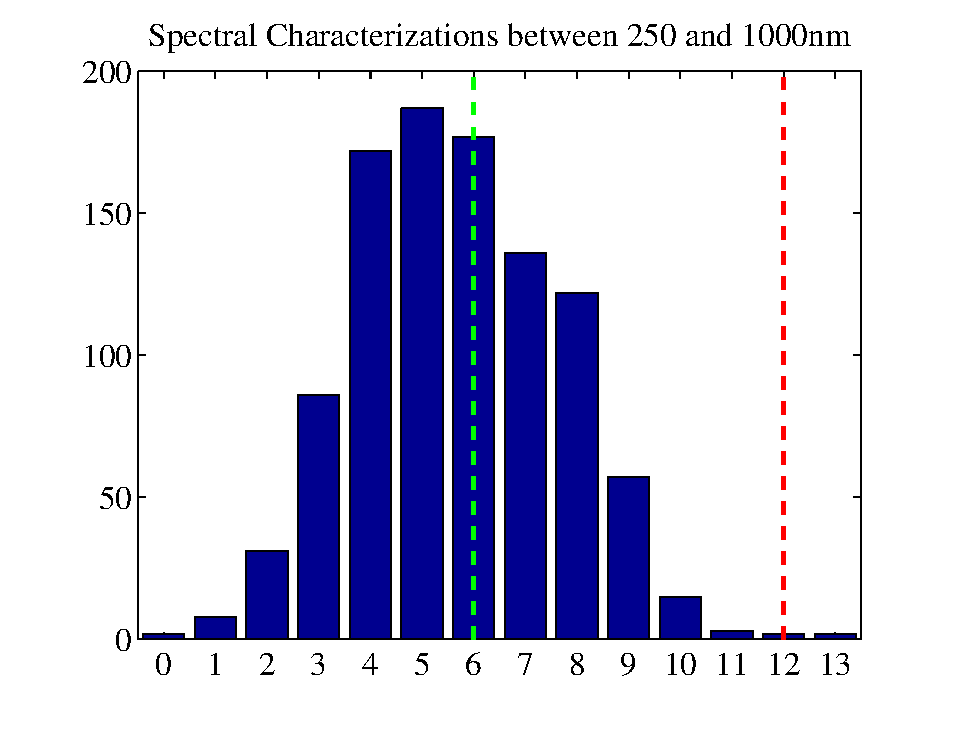
\includegraphics[width = 2.8in,clip=true,trim=0.4in 0in 0.5in 0in]{./figures/optimhistsd}
 \caption[Science yield from automated and randomized visit order]{ \label{fig:optim_hists} Comparison of science yield from automated and randomized visit order selection for 2 $\lambda/D$ coronagraph (top row) and THEIA (bottom row).  Blue bars are histograms of results from 1000 mission simulations using randomized visit order. Black dashed lines are results from the automated visit order with depth of search $k = 1$, red lines are results for automated visit order with $k = 3$, and  green lines represent timelines generated by selecting the next available highest completeness target.  In the spectral characterizations for the coronagraph, and both metrics for THEIA, the $k=1$ and $k=3$ cases produced identical results.}
 \end{figure}
 
\reffig{fig:optim_fuelvudets} shows a scatterplot of THEIA occulter fuel use vs.~the number of unique planets found for the 1000 randomized visit order missions and the automated visit order missions.  Here we do see a difference between the $k = 3$ and $k = 1$ simulations, with $k = 1$ producing a mission timeline where more fuel is used.  We compare only the amount of fuel used in slews, rather than total fuel use, since the stationkeeping fuel is directly linked to the number of observations and spectra and is automatically maximized along with these metrics.  This validation technique was applied to multiple randomly generated universes, with varying values of $\eta_\oplus$, producing similar results in each case.
\begin{figure}[ht]
\centering
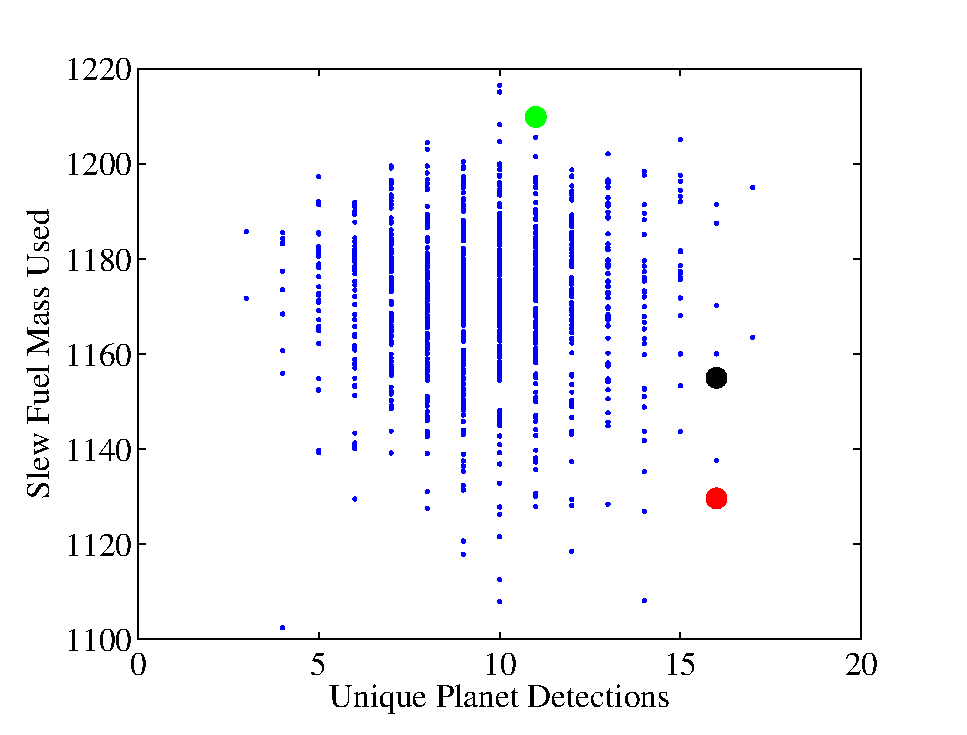
\includegraphics[width = 5in]{./figures/optim_fuelvudets}
 \caption[THEIA occulter propellant use]{ \label{fig:optim_fuelvudets} THEIA occulter propellant use (in kg) vs.~the number of unique planet detections for 1000 mission simulations using randomized visit order in one simulated universe.  The red point represents the mission timeline generated using the automated visit order for the same universe for $k = 3$, and the black point for $k = 1$.  The green point represents the timeline generated by selecting the next available highest completeness target.}
 \end{figure}

These results show that the automated mission does not represent a global optimum for these metrics.  There are a small number of missions which find more unique planets, or get more spectra.  However, we can see that the automated mission does a very good job of balancing these metrics and maximizing (or minimizing, in the case of fuel use) them jointly.  Allowing for the fact that the automated mission needs to be generated only once per universe, whereas a random walk search for local optima takes many trials, the benefits and efficiency of this approach become quite clear.  In terms of real mission planning, a random walk approach is simply not an option (since we only get one chance at scheduling the mission).  We also see that even when using a $k > 1$ (looking multiple steps into the future) gives us the same science yield as only considering one step, we still end up with a lower occulter fuel cost.  Finally, it is important to note that the margin between the unique planet detections using our scheduling algorithm versus the selection of the next available highest completeness target is smaller for the coronagraph than for THEIA, and is further from the tail of the distribution of randomized visit orders.  This is because the values for $a_i$ were fixed across all of the simulations here, and the $k$ values used are actually quite low for coronagraphs.  Optimizing the weights specifically for coronagraphs and using higher $k$ values produces improvements comparable to those seen in the occulter cases.

\begin{figure}[ht]
\centering
\includegraphics[width = 6in]{./figures/burnin}
 \caption[Science yield metric statistics as a function of ensemble size]{ \label{fig:burnin} Means and standard deviations for four metrics (total number of stars observed, number of unique stars observed, total number of planetary detections, number of unique planets detected) as a function of ensemble size.  These are normalized by the values for the full ensemble of 500 simulations.  Each simulation is of a 5 year THEIA mission with the default parameter set, with a universe of Earth-twins with $\eta_\oplus = 0.5$.}
 \end{figure}
Another important question is how many mission simulations are required so that the statistics extracted from the ensemble are accurate with high confidence.  It is difficult to make the case that the various metrics that we are interested in are approximately normally distributed, especially as many of them (such as the number of unique planets found) are discrete values, making it difficult to select a sample size corresponding to a specific confidence level.  However, this question can be answered empirically, by generating a large number of simulations and calculating distribution moments for the various metrics from subsets of these of varying size.  \reffig{fig:burnin} does exactly this, using 500 simulations of a 5 year THEIA mission with an Earth-twin population at a constant $\eta_\oplus$ of 0.5.  For all of these metrics (and others not plotted here), the sample mean and standard deviation converge to within 5\% of their respective values for the 500 simulation ensemble at around 100 samples.  This holds for a variety of configurations and instrument types, and so 100 samples is taken to be the minimum number required by the simulation framework.

\begin{figure}[ht]
 \centering
   \subfigure[]{\includegraphics[width=2.8in,clip=true,trim=0.4in 0in 0.5in 0in]{./figures/reldetsmult}  \label{fig:reldetsmult}}
   \subfigure[]{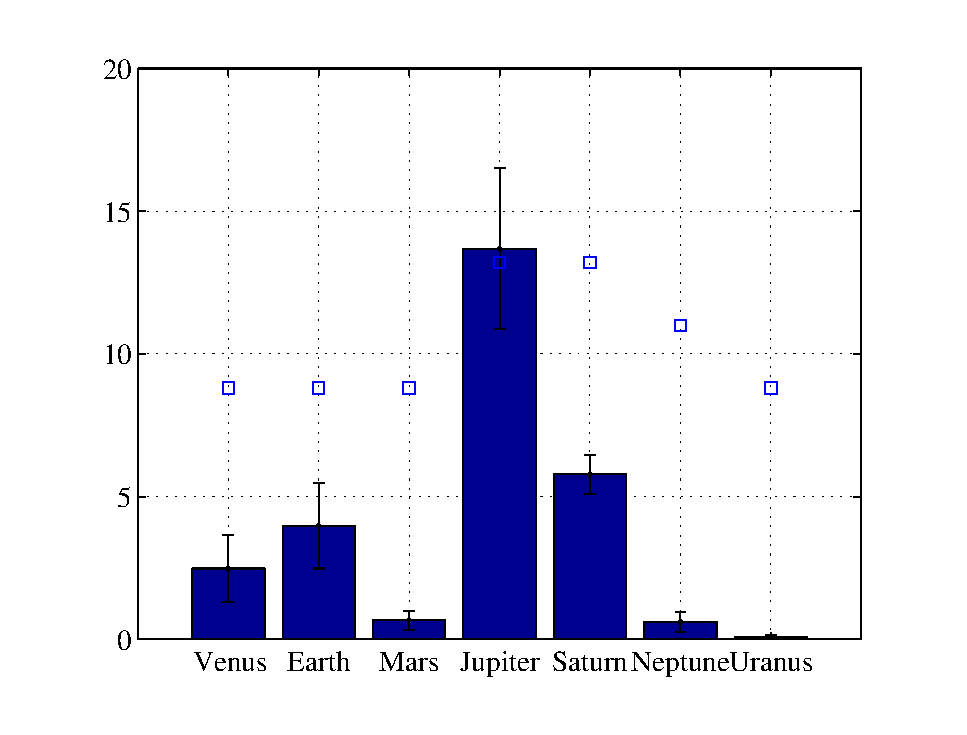
\includegraphics[width=2.8in,clip=true,trim=0.4in 0in 0.5in 0in]{./figures/mplanDets} \label{fig:mplandets}}
 \caption[Validation of Bayesian unique planet classification]{Results for 100 mission simulations using the 2 band photometry, 2 m O$_3$ configuration. (a) Total number of detections of each solar system planet analogue, normalized by the frequency with which they were simulated. This is used primarily as a test to ensure the multi-planet simulation capability is working as expected, but can also be useful in determining the relative detectability of the analogues - i.e., if Jupiters and Earths are distributed with equal frequency, O$_3$ should detect 4 times as many Jupiters as Earths, on average. (b) Average number of unique analogues found. Error-bars represent the standard deviation of the distribution. The squares indicate the average number of each analogue type that was included in the simulations.}
\end{figure}
Finally, in order to validate the multiple planet classification algorithm in \refeq{eq:bayesMultiPlanet}, we can generate systems populated with solar system planet analogues (as described in \S\ref{sec:gen_plan_sys}) and have the simulation algorithm classify detections made during repeat observations of targets where planets had previously been detected as newly discovered planets whenever the probability of a repeat detection is less than 50\%.   The test was run using a 44 star target pool with a 2 m telescope O$_3$ configuration and 2 band photometry required for each planet classified as a new detection.  Figure \ref{fig:reldetsmult} shows a histogram of the raw number of detections of each solar system planet analogue, normalized by the frequency with which they were simulated.  This is essentially the same as counting the total number of detections of each planet type in simulations where all of the analogues are selected with equal frequencies, and gives a sense of the relative detectability of the various planets in our solar system. 

As expected, Jupiter and Saturn-like planets, due to their size, relatively high albedo and placement, will be detected much more frequently than any other planet type.  Earths will be detected more frequently than Venus or Mars analogues due to their size and placement, and ice giants like Neptune will be difficult to detect unless they orbit much closer to their stars than Neptune does to the sun.  This histogram also implies that if Earth-twins and Jupiter-twins occur at the same rate in our universe, an observatory like O$_3$ should detect roughly four times as many Jupiters as Earths.  We can also use this data set to estimate the probability that a habitable zone candidate (i.e., a detection with an apparent separation less than the outer edge of the target star's HZ) actually is a habitable zone planet.  We find that if every exosystem was a scaled copy of the solar system, HZ candidates would represent about 22\% of all detections, and would actually be Earth analogues 43\% of the time.  They would be rocky planet analogues (Venus, Earth, or Mars) 83\% of the time, and giant planet analogues (Jupiter, Saturn, or Uranus) 17\% of the time.

Figure \ref{fig:mplandets} shows the average number of each planet analogue classified as unique over 100 simulations.  The algorithm correctly identified planets as new detections in approximately 60\% of applicable cases (detections during repeat observations of targets with prior detections).  This led to the apparent discovery (according to the algorithm's internal bookkeeping) of approximately 45\% of included Earth-like planets, whereas earlier single-planet system studies indicate that this value should be less than 33\%.  At the same time, according to the algorithm's classification, it discovered slightly more Jupiters, on average, than were included in the simulation, while in reality the true average rate of discovery was closer to 85\%. Because of the limited target pool size, each star in the  pool was observed at least once in most of the simulation instances, and the high visibility of Jupiter analogues made them easy to detect.  

\subsection{Results}
For each instrument an ensemble of mission simulations was generated over simulated universes containing only Earth-twin planets, a fixed mission length of 5 years, and fixed target lists selected from a pool of real stars within 30pc of the solar system.  Each ensemble consists of 1000 simulations with varying assumed frequencies of Earth-like planets ($\eta_\oplus$). Figures \ref{fig:compinsts4m} to \ref{fig:compinsts16m} show the median values of the four science yield metrics for the four instrument designs for telescopes with circular apertures of 4, 8 and 16m diameters.  The error-bars represent the one-sided deviations of each distribution.  No SDO was evaluated for the 16m telescope because the starshade is so large that little significant science can be achieved during a 5 year mission with the propulsion system used here.  Results for O$_3$ are plotted separately since O$_3$ does not have a spectral characterization capability, making it difficult to compare directly with the other instruments that do.  The lines in the various plots represent median values for 100 simulations at each value of $\eta_\oplus$.  Error-bars represent the one-sided deviations of each distribution.  `All Detections'  are the total number of planets found (including multiple detections of the same planet), `Unique Detections' are the number of unique planets found, and `Unique Targets' are the number of unique target systems visited during the mission.

\begin{figure}[ht]
 \begin{center}
  \begin{tabular}{c c}
   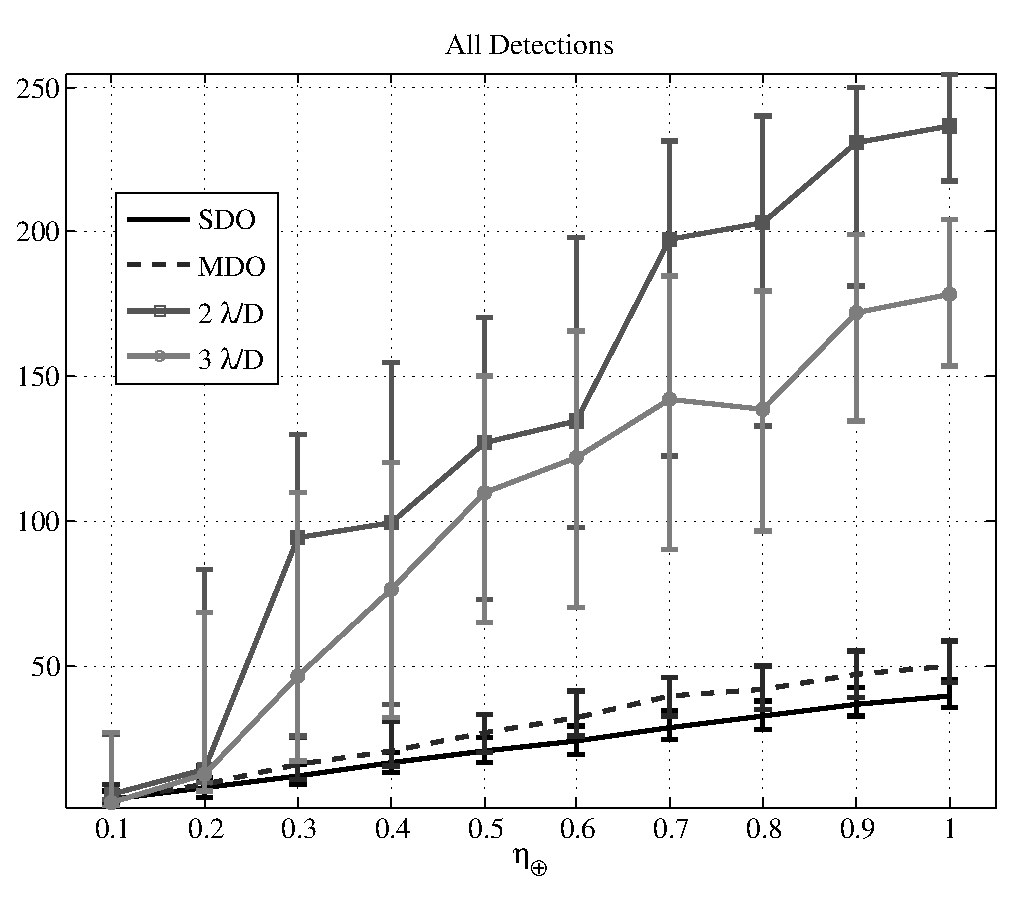
\includegraphics[width=2.9in]{./figures/c4m_ADETs} &
   \includegraphics[width=2.9in]{./figures/c4m_AuDETs} \\
   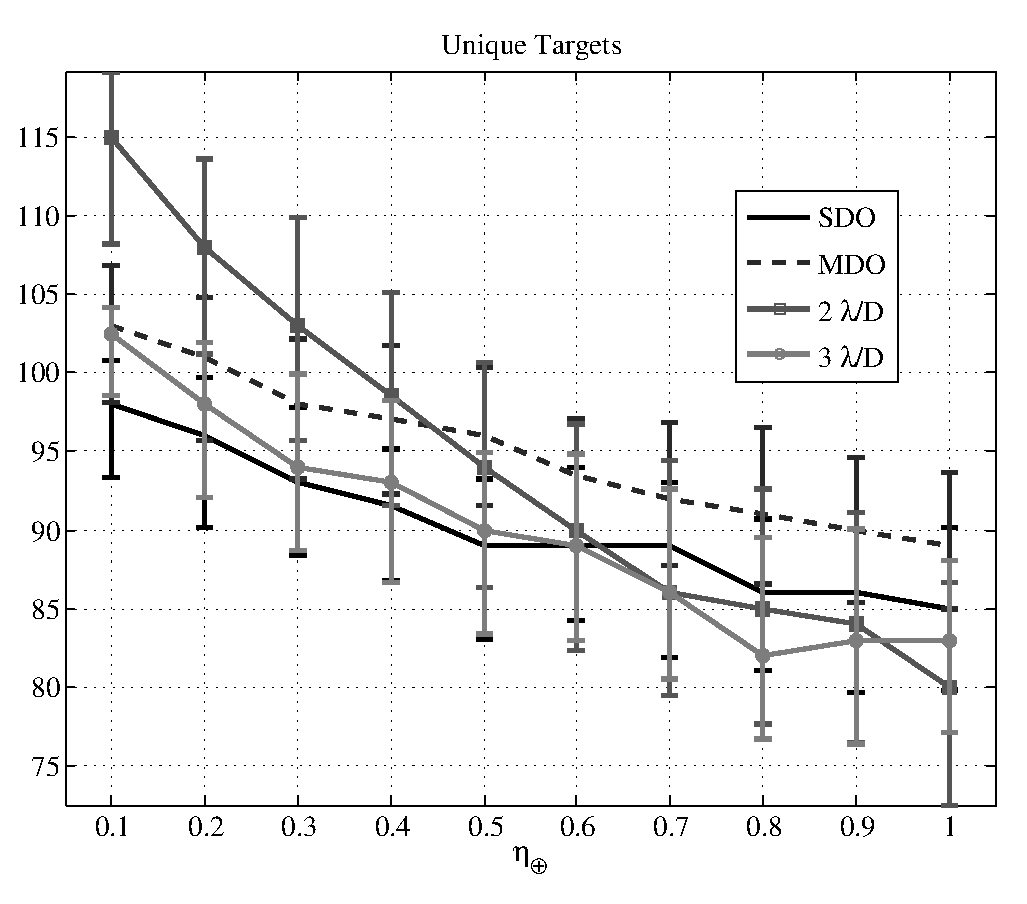
\includegraphics[width=2.9in]{./figures/c4m_Auvisits} &
   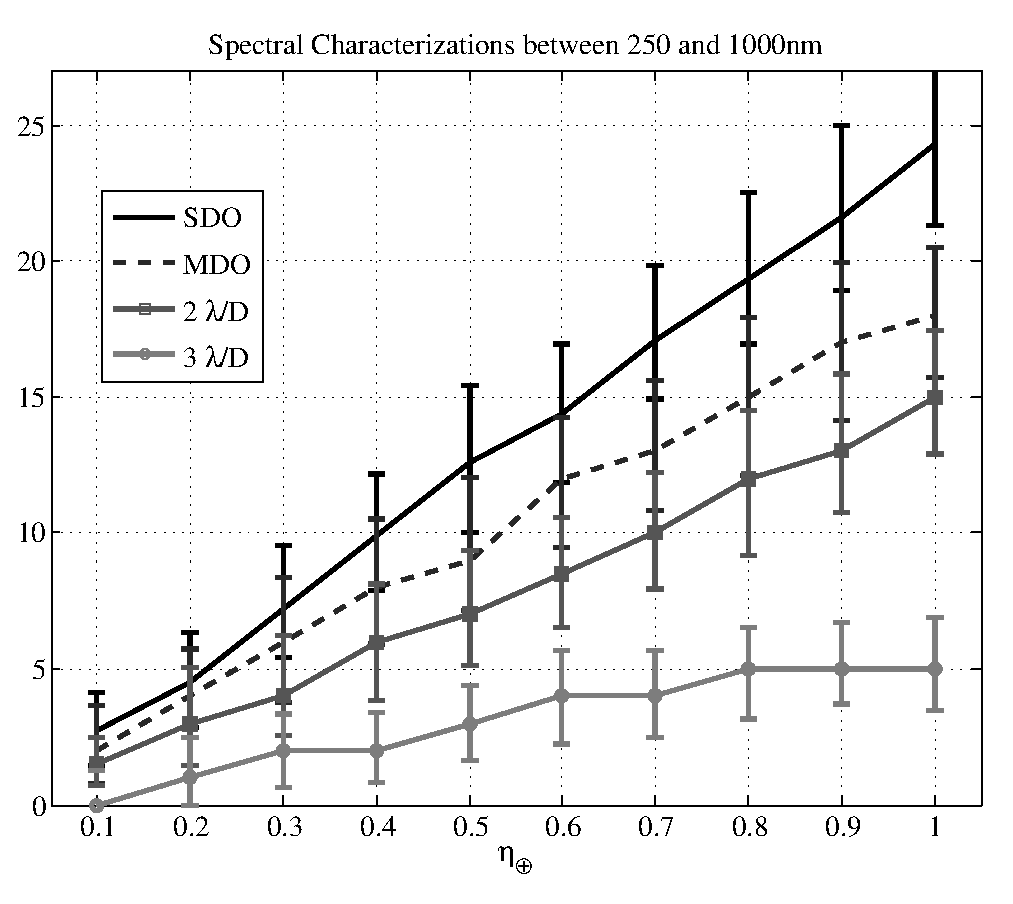
\includegraphics[width=2.9in]{./figures/c4m_ASPECTRA}
  \end{tabular}
 \end{center}
 \caption[4 m telescope comparison]{ \label{fig:compinsts4m} Simulation results for the SDO, MDO, and the 2 and 3 $\lambda/D$ coronagraph mission concepts as functions of $\eta_\oplus$ with a 4 m telescope for Earth-twin planetary populations.}
 \end{figure}
 
 These figures illustrate perfectly the inherent tradeoff between telescope size and achievable science with an occulter.  As larger starshades become necessary, unless there is a significant improvement in the propulsion system, the science yield for a fixed mission length decreases.  Although it is possible to achieve higher thrust with more power this requires increasing the size and mass of the power subsystem, and leads to another tradeoff.  This trade study is an important future task, and one for which this framework is well suited.
 
\begin{figure}[ht]
 \begin{center}
  \begin{tabular}{c c}
   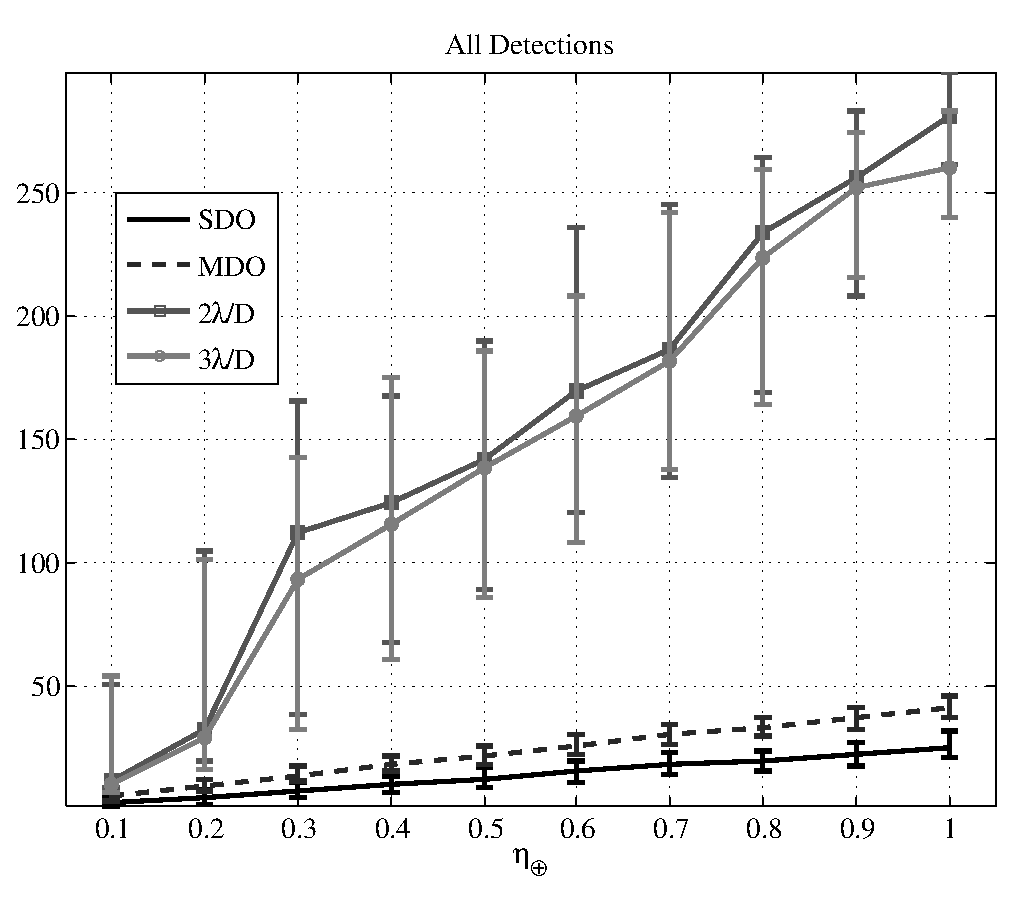
\includegraphics[width=2.9in]{./figures/c8m_ADETs} &
   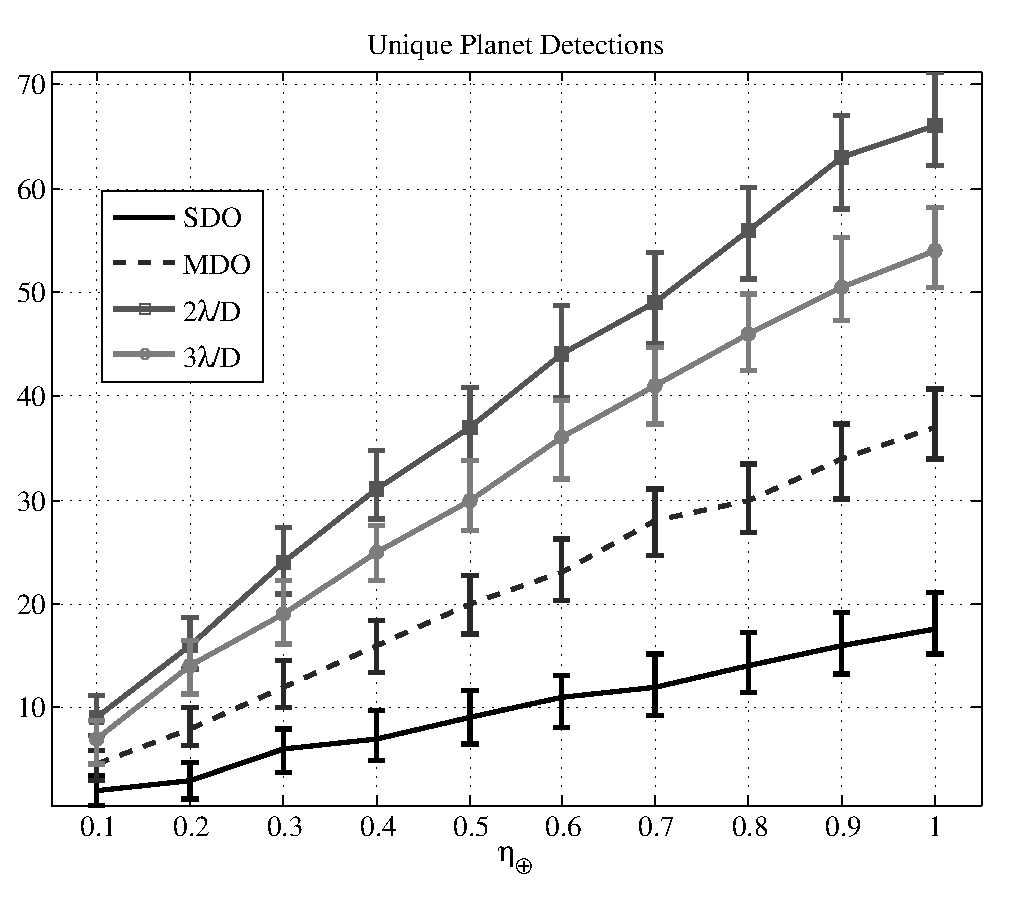
\includegraphics[width=2.9in]{./figures/c8m_AuDETs} \\
   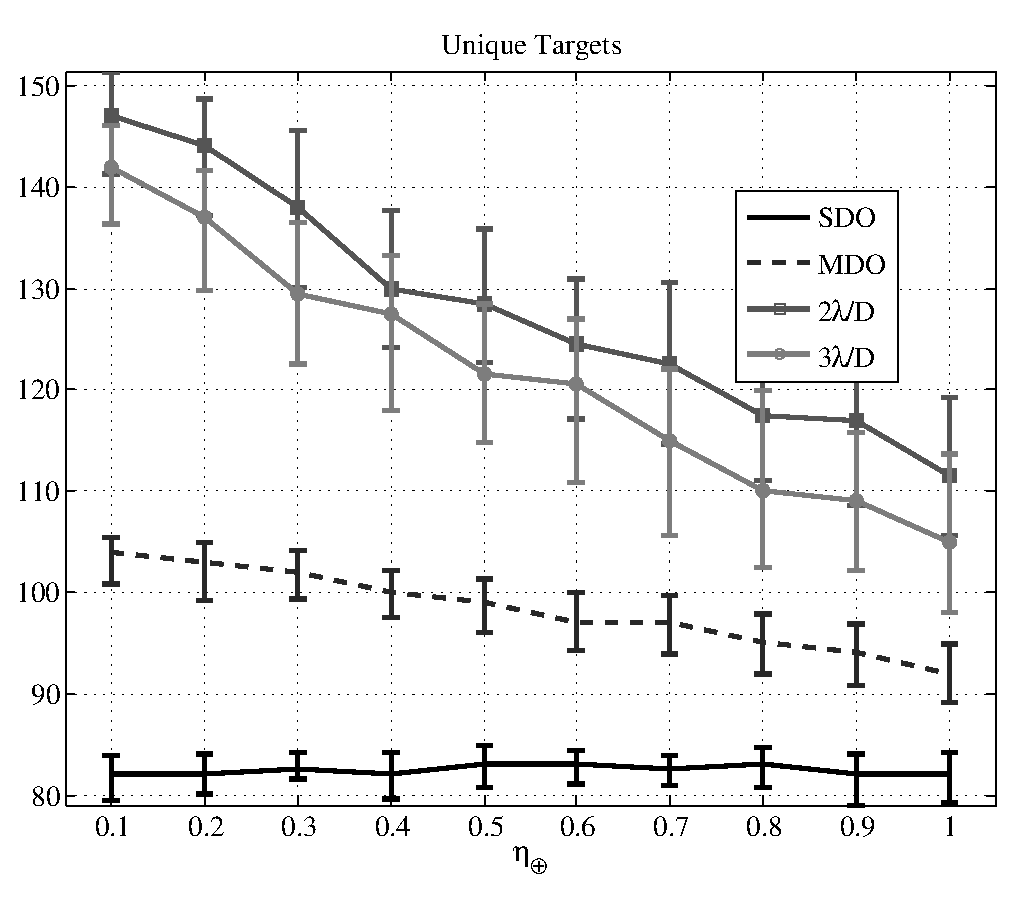
\includegraphics[width=2.9in]{./figures/c8m_Auvisits} &
   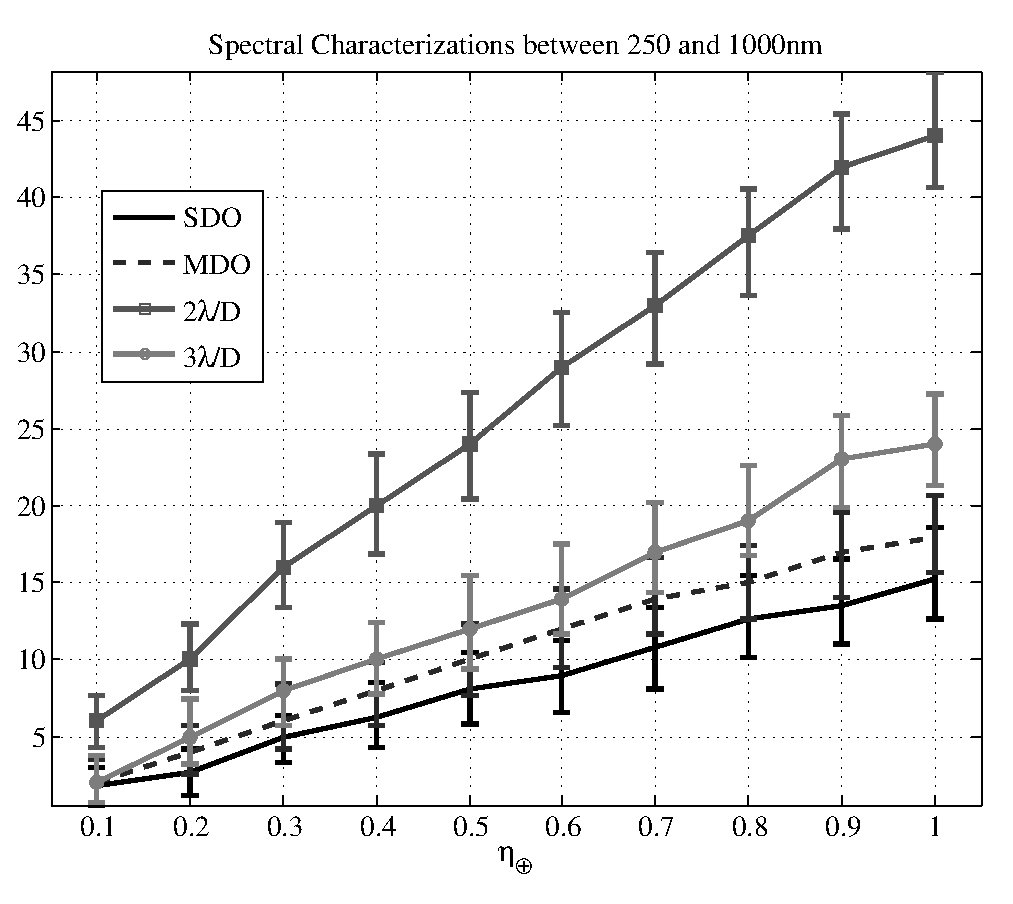
\includegraphics[width=2.9in]{./figures/c8m_ASPECTRA}
  \end{tabular}
 \end{center}
 \caption[8 m telescope comparison]{ \label{fig:compinsts8m} Simulation results for the SDO, MDO, and the 2 and 3 $\lambda/D$ coronagraph mission concepts as functions of $\eta_\oplus$ with an 8 m telescope for Earth-twin planetary populations.}
 \end{figure}
 
 At the 4m scale, the occulter and coronagraph mission concepts are competitive in different science yield metrics.  For total number of detections, the coronagraphs are the clear winners, with many times as many detections as either of occulter designs.  These results may be slightly misleading, since they represent, for the most part, many repeated detections of a small number (usually fewer than 5) of highly visible planets.  However, this demonstrates the advantage of being able to perform many more observations over the course of the mission and, with improvements to the scheduling algorithm, should be translatable into a larger number of orbital fits for the coronagraphs.  The two occulters average less than two detections per unique planet found, which means that they are generally unable to get more than one orbital fit in five years of mission time.

For unique planet detections, the two occulters perform almost identically, finding about 10\% fewer planets than the 2 $\lambda/D$ coronagraph and 25\% more than the 3 $\lambda/D$ coronagraph at $\eta_\oplus = 1$.  This result is almost purely a function of having a limited target list---in a universe with a uniform distribution of isotropically positioned stars, we would expect the coronagraphs' larger total number of observations over the mission lifetime to produce proportionately more unique detections.  As we are limited to existing stars, all of the instruments are able to find all of the easily observable planets within five years and the greater number of visits made by the coronagraphs translates into only a few more unique detections. At this telescope scale, all of the designs consistently find fewer than half of the available planets in a given universe.  
 
 \begin{figure}[ht]
 \begin{center}
  \begin{tabular}{c c}
   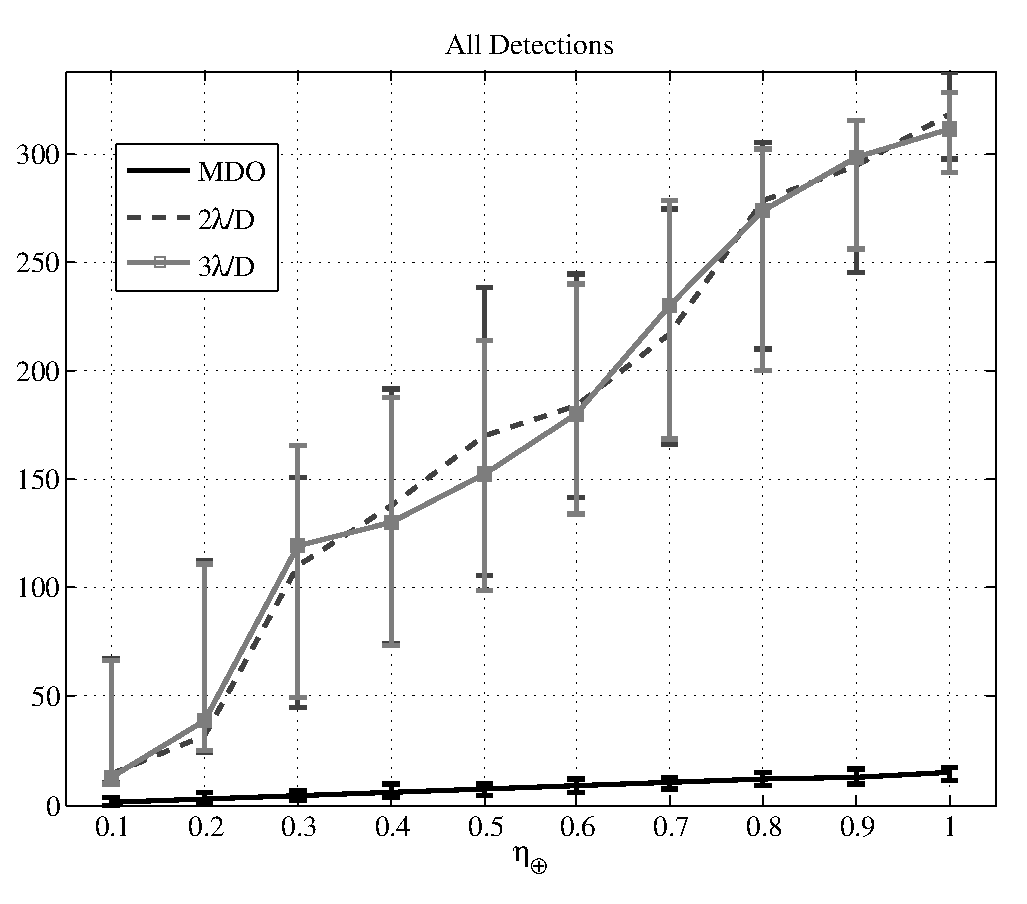
\includegraphics[width=2.9in]{./figures/c16m_ADETs} &
   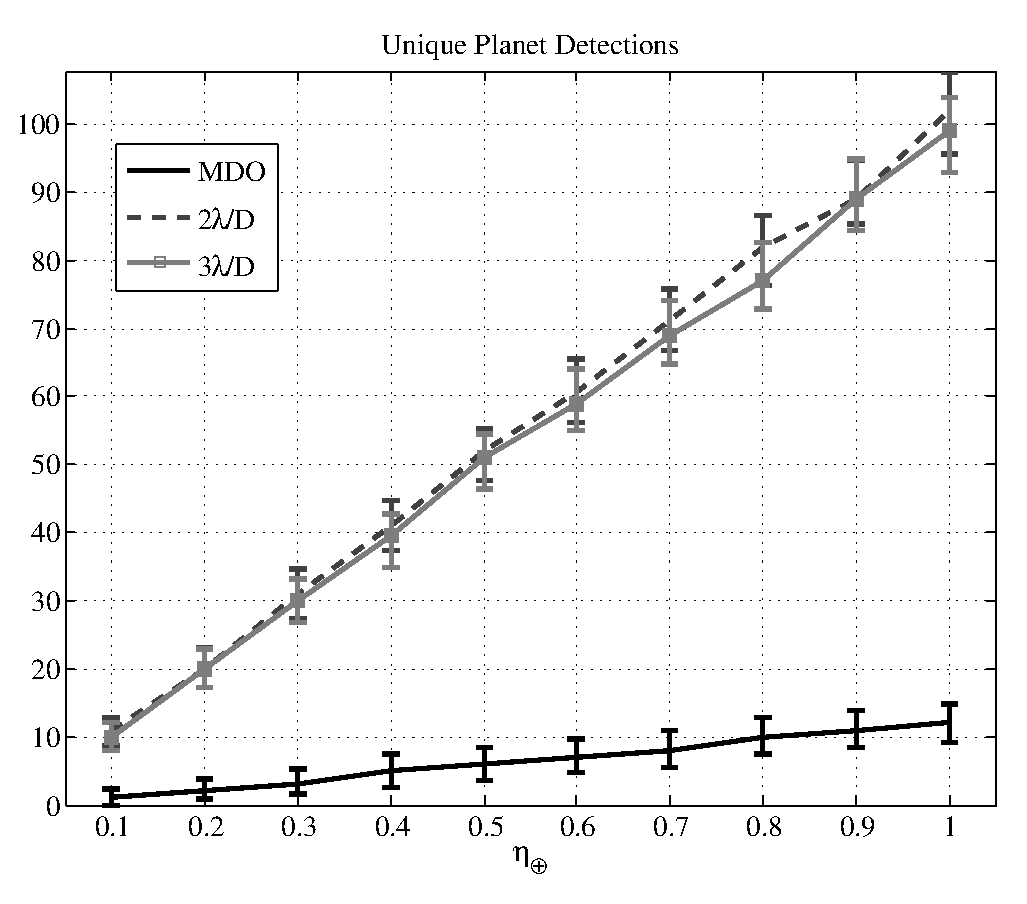
\includegraphics[width=2.9in]{./figures/c16m_AuDETs} \\
   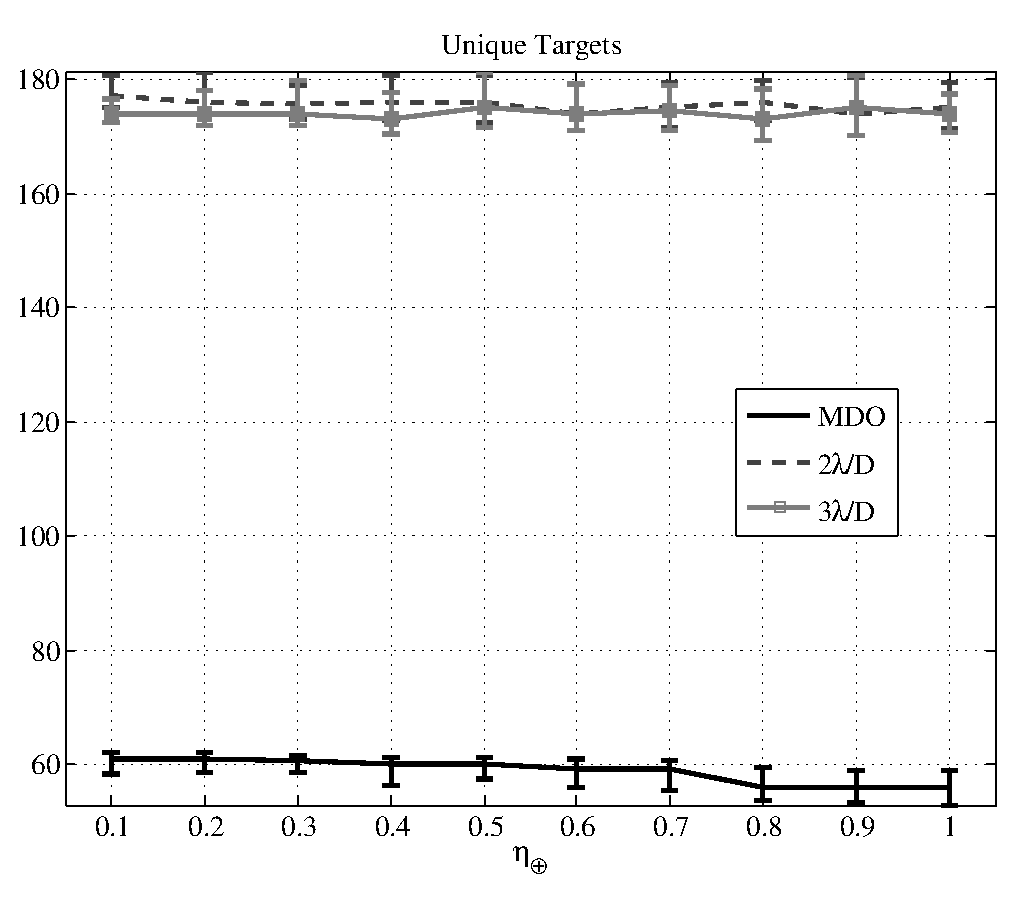
\includegraphics[width=2.9in]{./figures/c16m_Auvisits} &
   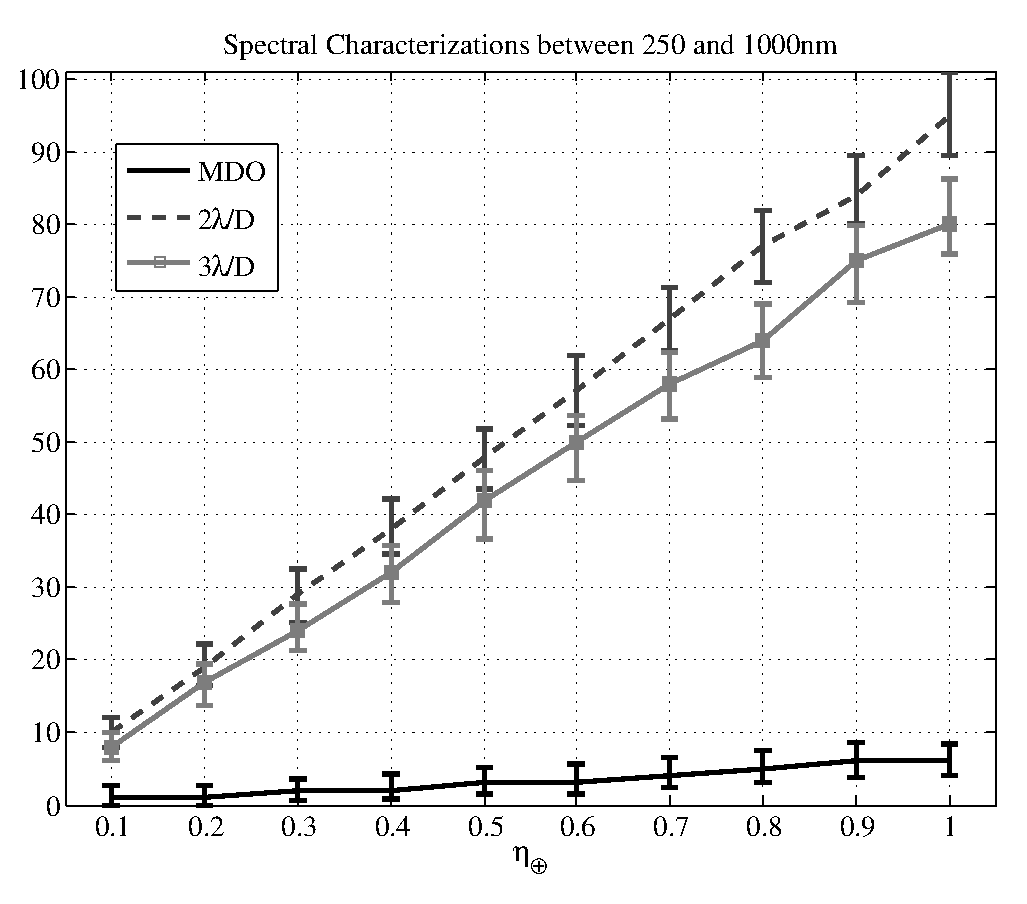
\includegraphics[width=2.9in]{./figures/c16m_ASPECTRA}
  \end{tabular}
 \end{center}
 \caption[16 m telescope comparison]{ \label{fig:compinsts16m} Simulation results for the MDO, and the 2 and 3 $\lambda/D$ coronagraph mission concepts as functions of $\eta_\oplus$ with a 16 m telescope for Earth-twin planetary populations.}
 \end{figure}

The coronagraphs' large number of detections is balanced by their relatively poor performance in terms of spectral characterization.  Because of their wavelength dependent IWA, and the fact that detections for Earth-like planets will occur at relatively low separations\cite{brown2005}, in most cases the coronagraphs are capable of only a partial spectrum between 250 and 1000 nm.  We see that the $2\lambda/D$ gets slightly fewer full spectra than the MDO (which has difficulties getting full spectra due to the extra required slew for the longer wavelength characterizations), but both are outperformed by the single distance occulter.  The 3 $\lambda/D$ coronagraph is highly IWA limited, and gets many fewer full spectra than any of the other designs.  From these metrics, we can conclude that for a 4 m telescope, coronagraphs and occulters are both viable options, as long as a 2 $\lambda/D$ IWA is achievable, and that the decision as to which instrument to build should be made based on other considerations, including the relative difficulties of wavefront control versus starshade manufacturing and positioning.
 
 For the 8 m telescope, we start to see significant disparity between occulter and coronagraph performance, due completely to the smaller amount of observation time available to the occulters as more time is spent slewing between targets.  Even so, the occulter designs still produce non-negligible science yield, with the MDO finding as many as 37 unique planets at $\eta_\oplus = 1$.  The MDO is now outperforming the SDO, since the starshade required to cover the entire spectral band at one separation distance is much larger than the MDO.  At this scale, coronagraphs clearly produce higher yields in all four science metrics.  However, the problems of telescope stability and wavefront control become more difficult with larger telescopes.  It may turn out that achieving even 3 $\lambda/D$ is exceedingly difficult.  If this is the case, then occulter are still a viable alternative, even if there are no improvements in propulsion technology beyond what is modeled here.
 
 \begin{figure}[ht]
 \begin{center}
  \begin{tabular}{c c}
   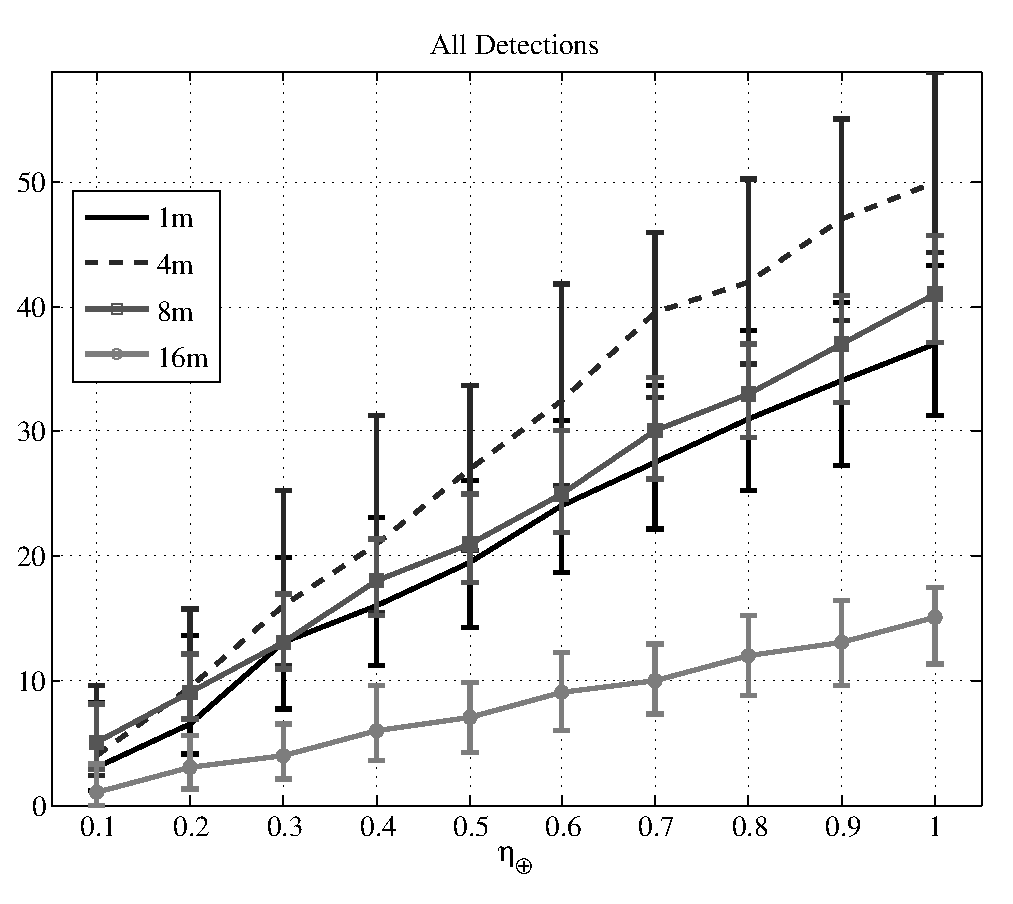
\includegraphics[width=2.9in]{./figures/occulters_ADETs} &
   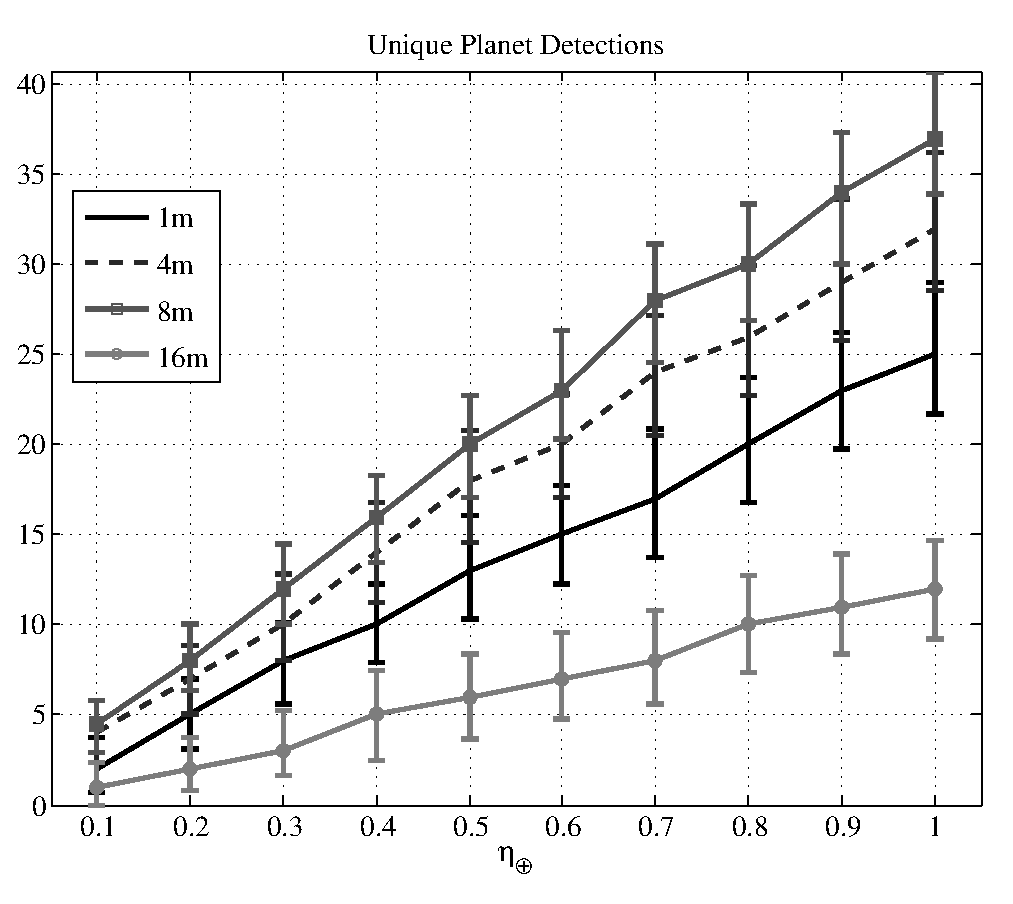
\includegraphics[width=2.9in]{./figures/occulters_AuDETs} \\
   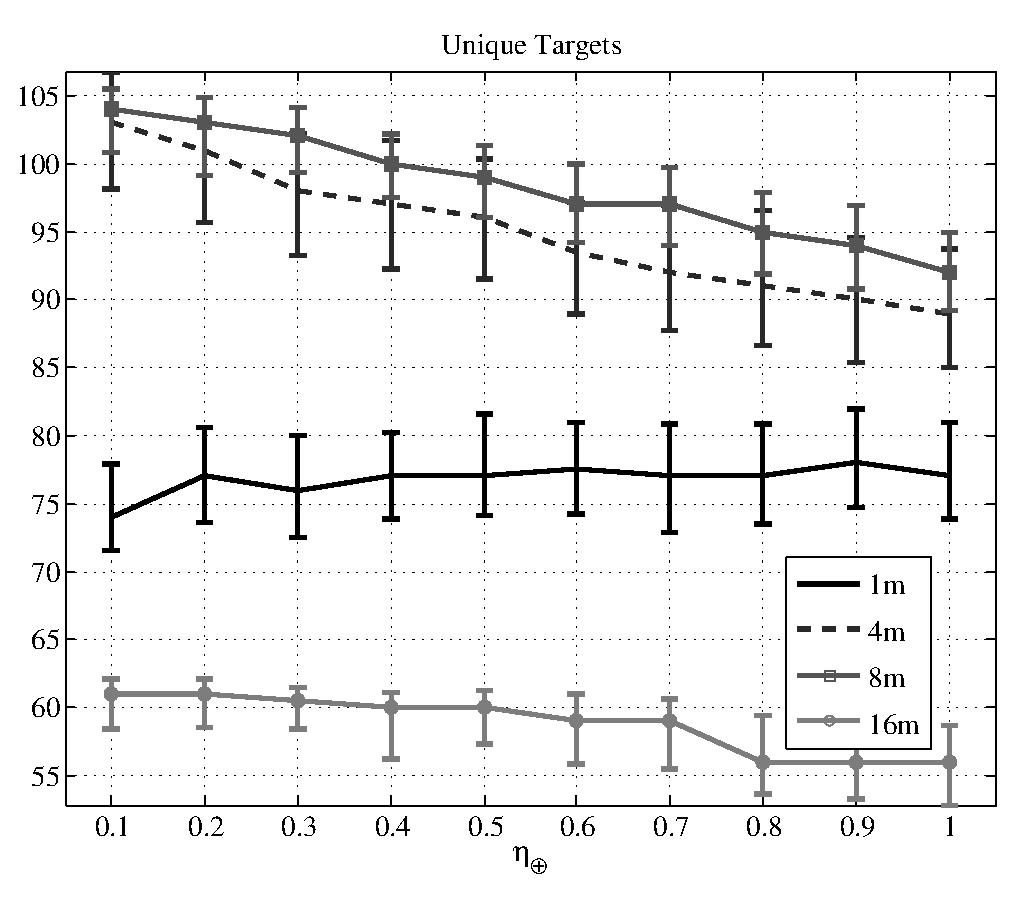
\includegraphics[width=2.9in]{./figures/occulters_Auvisits} &
   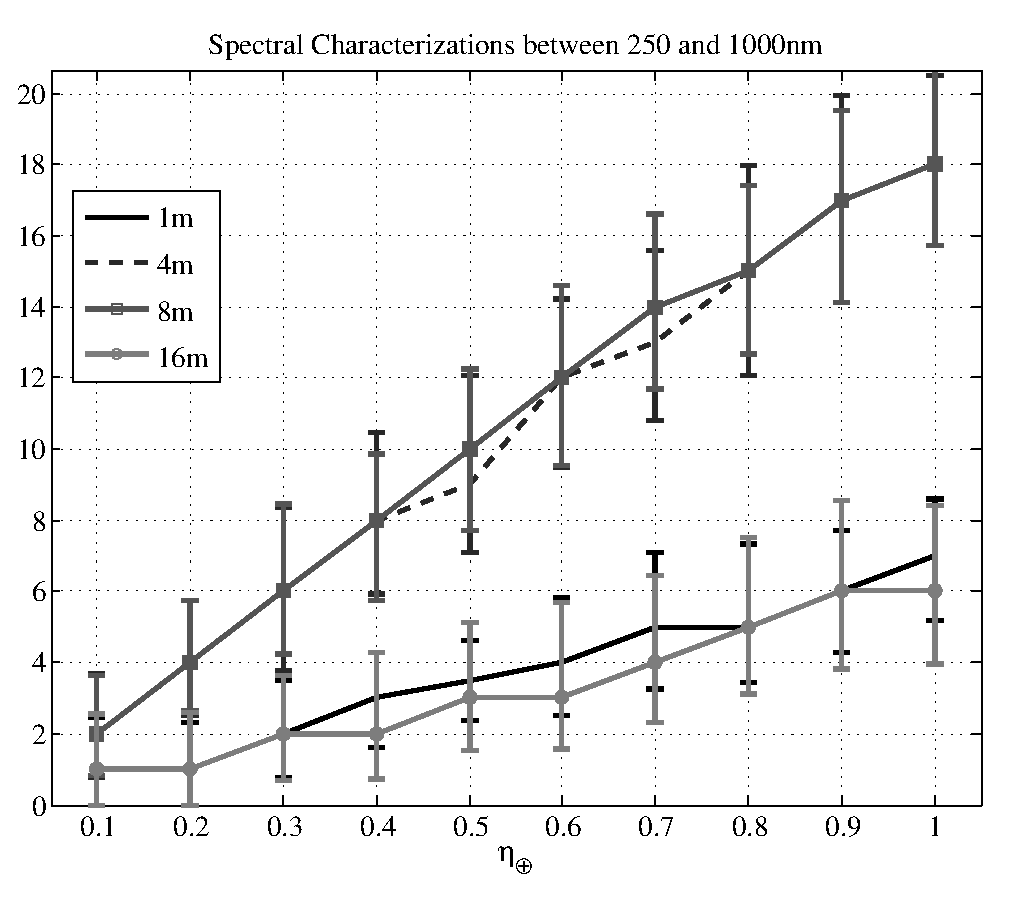
\includegraphics[width=2.9in]{./figures/occulters_ASPECTRA}
  \end{tabular}
 \end{center}
 \caption[MDO comparison]{ \label{fig:compMDOs} Simulation results for MDOs with 1, 4, 8, and 16 m telescopes for Earth-twin planetary populations.}
 \end{figure}
 
 With the 16m telescope, the disparity between coronagraphs and occulters is so great that it becomes very difficult to argue for the benefits of an occulter, as modeled here.  The extremely large starshade required even by the MDO makes transit slews take so long that less than 5\% of a mission is typically spent on observation. This leads to multiple instances of zero detections at lower values of $\eta_\oplus$, meaning that this mission design could be a complete failure in terms of finding planets in this population.  Of course, these results would be very different if we considered a system of multiple starshades operating with one telescope, as proposed in \citet{hunyadi2007a}.  With each additional starshade, the average transit slew time decreases, improving the science yield.  In fact, one can design a constellation of starshades such that there is a guaranteed maximum retargeting time, in which case the occulter would operate much like a coronagraph system, with near constant overhead time per observation.  Compared with an 8 or 16 m  telescope, the cost of each starshade is relatively low, making multiple starshades a reasonable approach.  Thus, we conclude that at current propulsion technology levels, an occulter system with a single starshade is not a suitable starlight suppression system for telescopes greater than 8m in diameter.  The coronagraphs continue to perform well at the larger scales, with the wavelength dependence of the IWA becoming much less of a problem for this specific planetary population

 \reffig{fig:compMDOs} compares all of the MDO designs, including one for a 1m telescope.  This 1 m telescope is different from O$_3$\,---it does not represent a developed mission concept, but rather what would happen if you were to use the THEIA occulter with a 1 m telescope and all of the same mission rules.  It is not intended to represent a viable mission concept (unlike O$_3$) but merely to test whether any useful science can be achieved with an occulter at aperture sizes where classical coronagraphs are essentially useless for terrestrial planet-finding.  At 1 m, the IWA at even the telescope's diffraction limit would completely cover the habitable zone for most target stars.  Since the occulter's IWA is determined solely by the starshade geometry, this problem does not exist for the occulter, although the smaller aperture size makes integration times much larger.  The same size starshade is required for both the 1 and 4 m telescopes because the smaller telescope aperture spreads the point spread function, requiring a relatively larger level of suppression to produce the required contrast at the same IWA. The scheduling algorithm is able to produce a surprisingly large number of detections with the 1m MDO (about 20\% fewer than the 4 m MDO) by visiting a smaller number of unique target stars during the mission.  Of course, there is no way to get around the longer integration times required by the smaller telescope aperture, which means that the 1 m MDO gets relatively few spectra in the course of a mission, performing on par with the 16 m version.  However, these results show that good science is possible with smaller telescopes, and led to the development of the O$_3$ concept.  
 
 \reffig{fig:compcorons} compares all of the coronagraph designs, showing the progressive improvements in all metrics with telescope size, and the decreasing importance of the IWA wavelength dependence for this planetary population. 
 \begin{figure}[ht]
 \begin{center}
  \begin{tabular}{c c}
   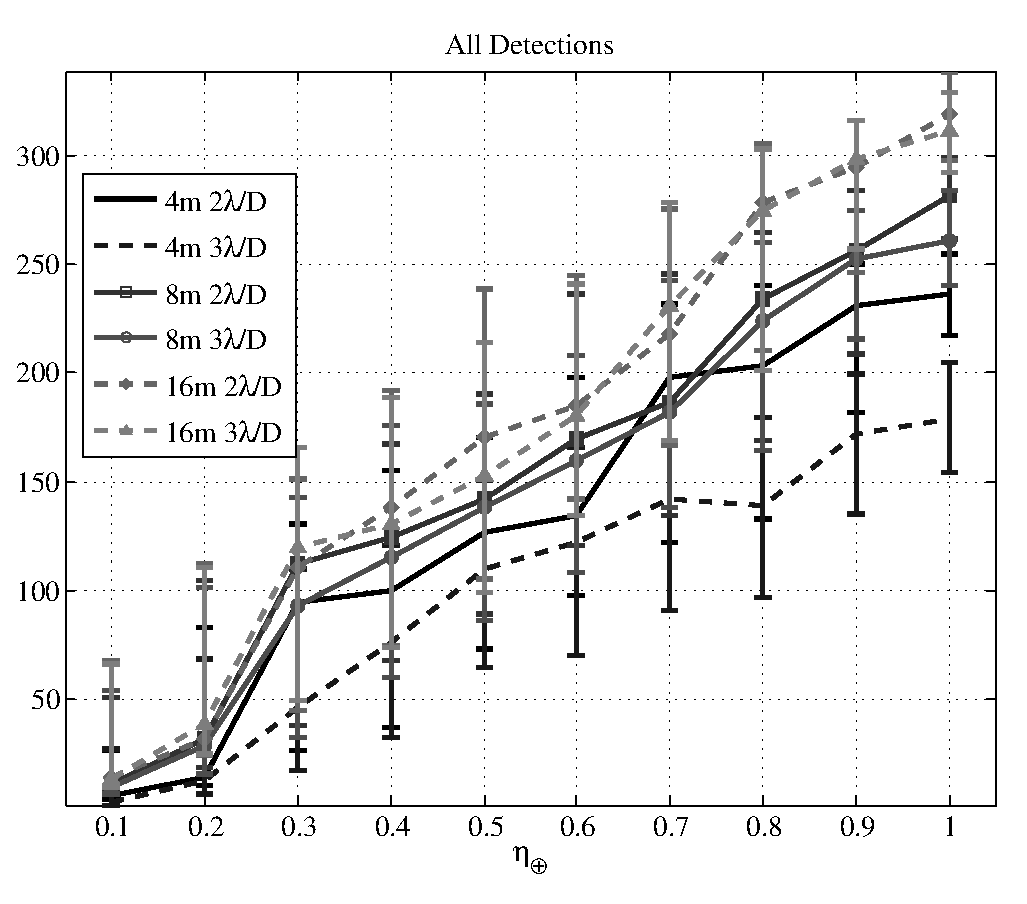
\includegraphics[width=2.9in]{./figures/coronagraphs_ADETs} &
   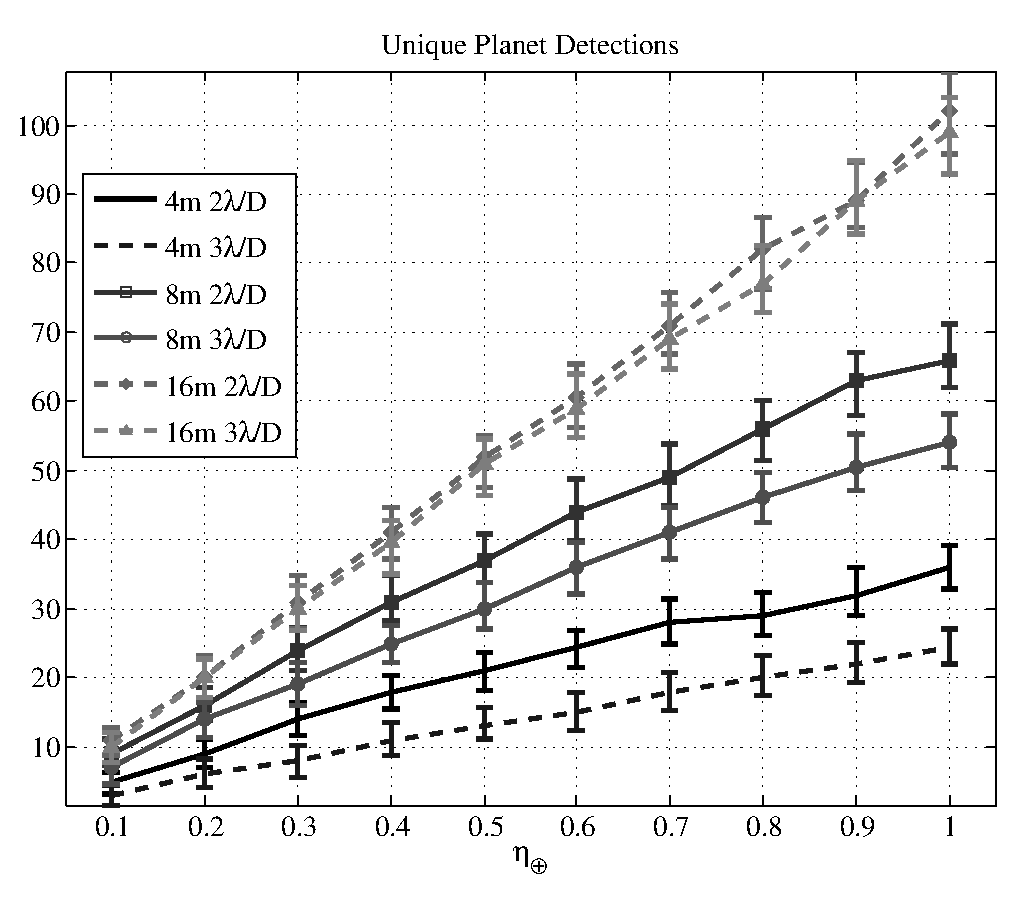
\includegraphics[width=2.9in]{./figures/coronagraphs_AuDETs} \\
   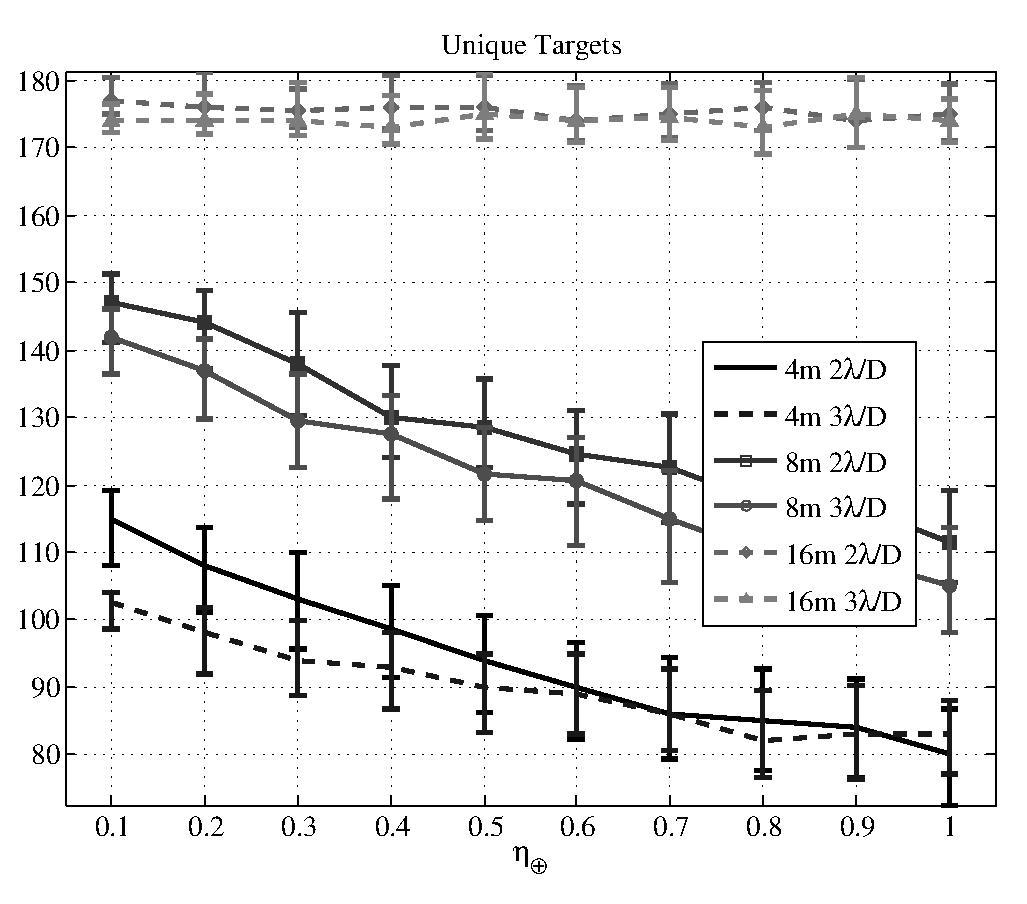
\includegraphics[width=2.9in]{./figures/coronagraphs_Auvisits} &
   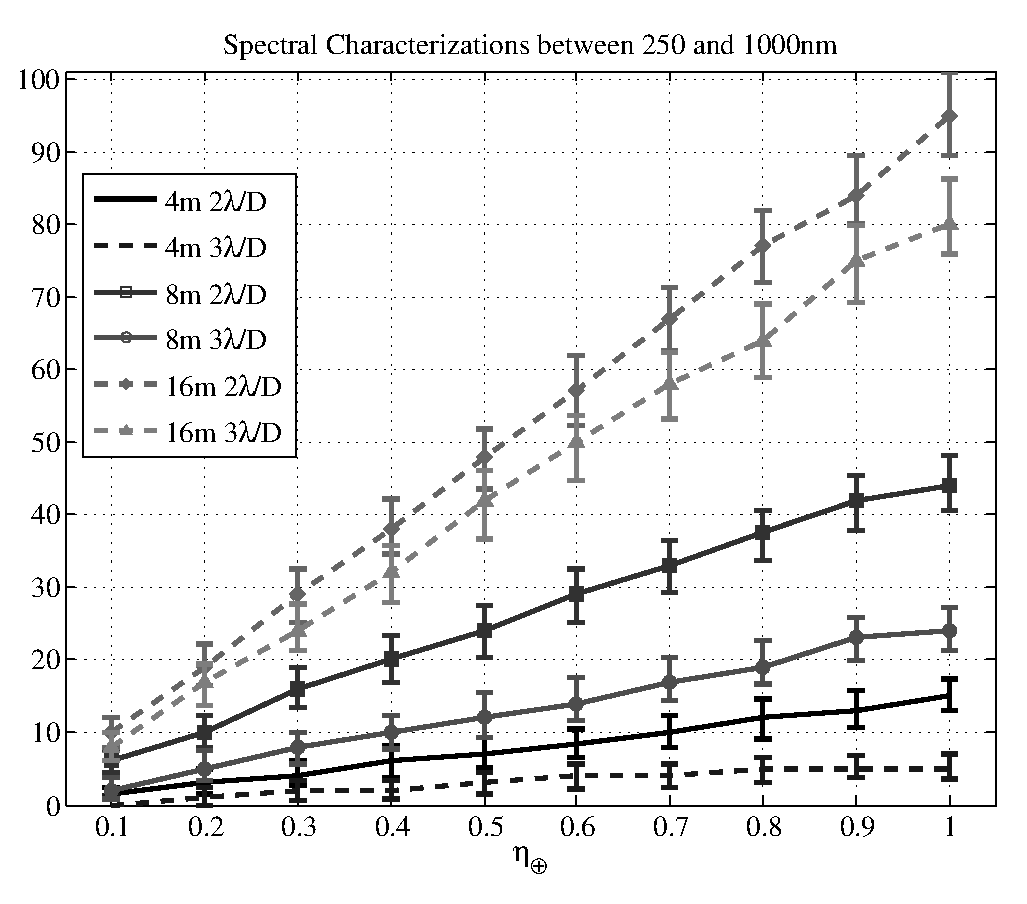
\includegraphics[width=2.9in]{./figures/coronagraphs_ASPECTRA}
   \end{tabular}
 \end{center}
 \caption[Coronagraph comparison]{ \label{fig:compcorons} Simulation results for coronagraphs with 4, 8, and 16 m telescopes for Earth-twin planetary populations.}
 \end{figure}
 Because both the MDOs split spectral characterizations into two sub-bands, and the largest observable wavelength for coronagraphs changes with distance for different targets, we can also track the number of spectra characterizations that cover less than the whole band.  \reffig{fig:pspectra} shows the total number of spectra to at least 700 nm collected by the various occulters and coronagraphs.  The trends here are quite similar to those in the full spectra plots.  As before, the 4 m occulter greatly outperforms its coronagraph counterpart.
   \begin{figure}[ht]
 \centering
\subfigure[Coronagraphs]{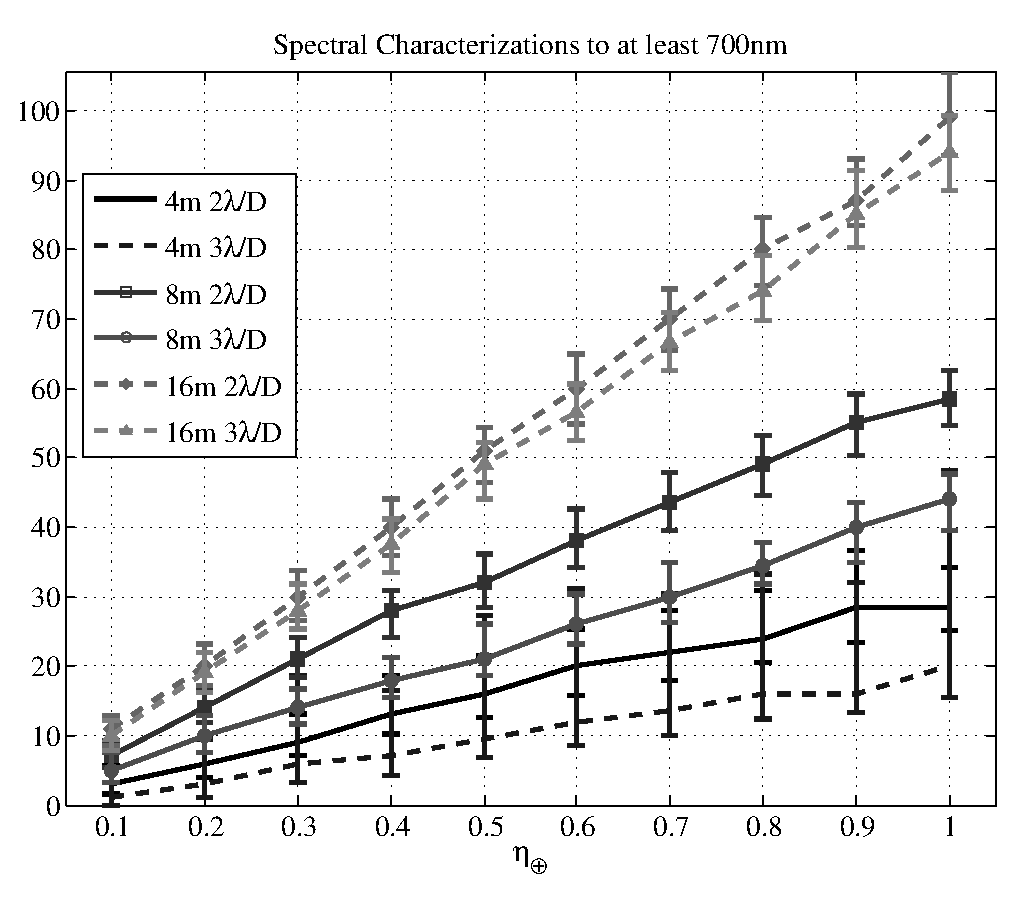
\includegraphics[width=2.9in]{./figures/coronagraphs_PSPECTRA}}
\subfigure[MDOs]{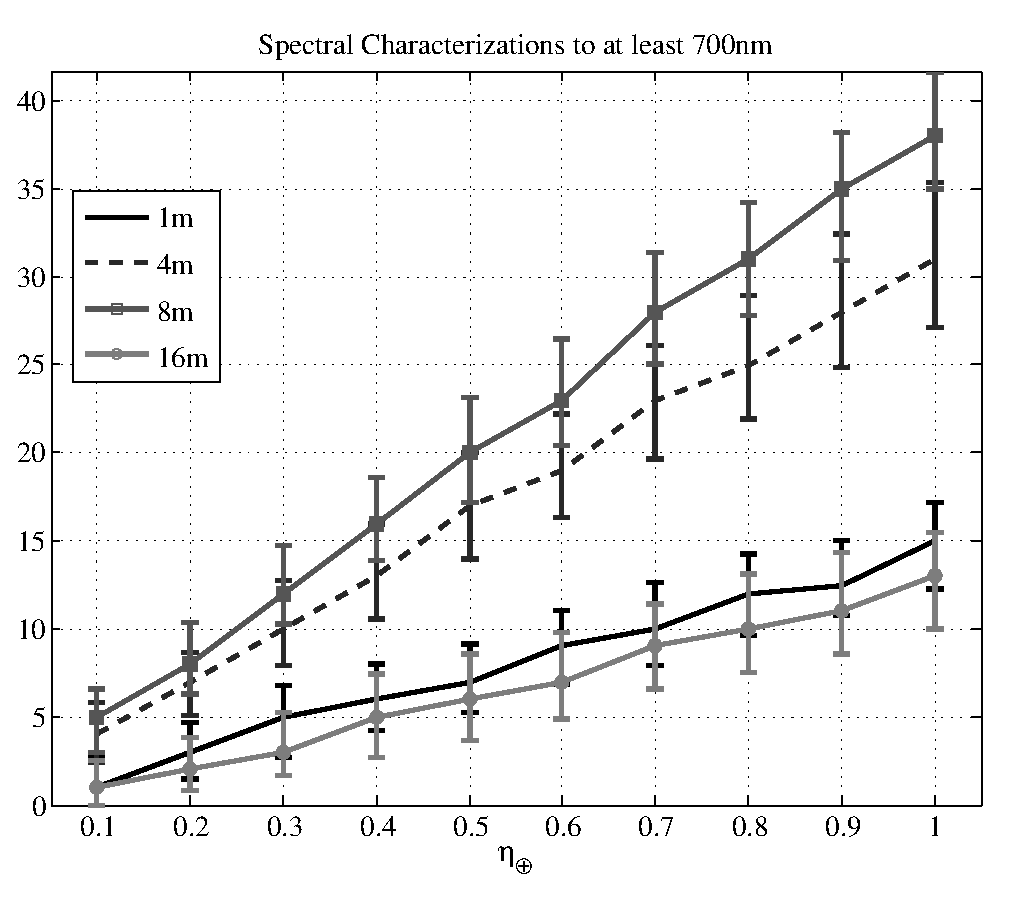
\includegraphics[width=2.9in]{./figures/occulters_PSPECTRA}}
\caption[Partial spectra]{ \label{fig:pspectra} Total number of partial spectra (to at least 700 nm) collected for instruments at varying telescope scales.}
 \end{figure}
 
 We can also compare the total amount of time devoted to planet-finding observations by all of these instruments. \reffig{fig:obsTimes} demonstrates two clear trends: As the telescope aperture size increases, more photons are collected requiring less integration to achieve the same S/N, and so the total observation time generally decreases with aperture size.  In addition, for occulters, as the telescope size grows, so does the size (and mass and separation distance) of the starshade, meaning that more time is needed to move the occulter between observations, so the total observation time is further decreased with increasing telescope aperture size.  This is illustrated particularly well by the 1 m occulter, which uses the same starshade as the 4 m and has significantly larger total observation times.  Another trend common to both instrument types is the increase in observation time with $\eta_\oplus$ as higher occurrence rates of planets will lead to more spectral characterizations and longer total integration times.  The one exception to this is the larger occulters, which actually have almost constant integration times for all $\eta_\oplus$ as so much of their mission time is devoted to slewing the occulter.
  \begin{figure}[ht]
 \centering
\subfigure[Coronagraphs]{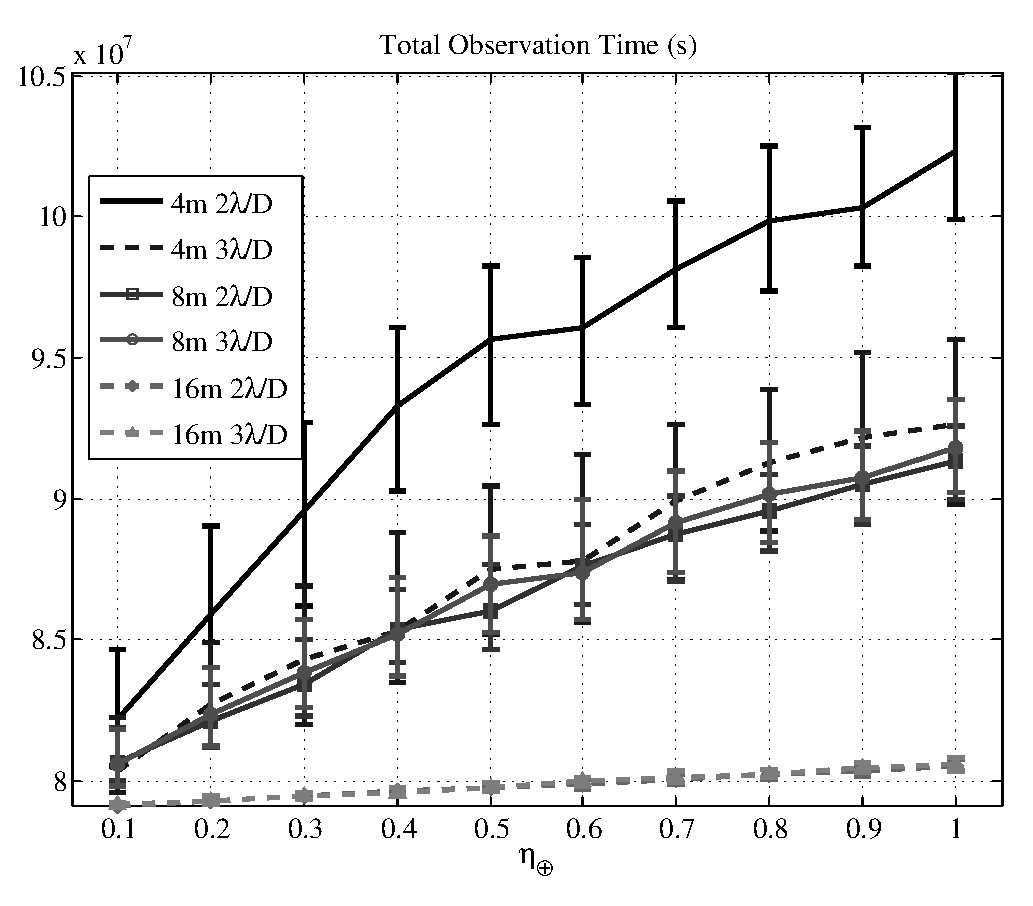
\includegraphics[width=2.9in]{./figures/coronagraphs_obstime}}
\subfigure[MDOs]{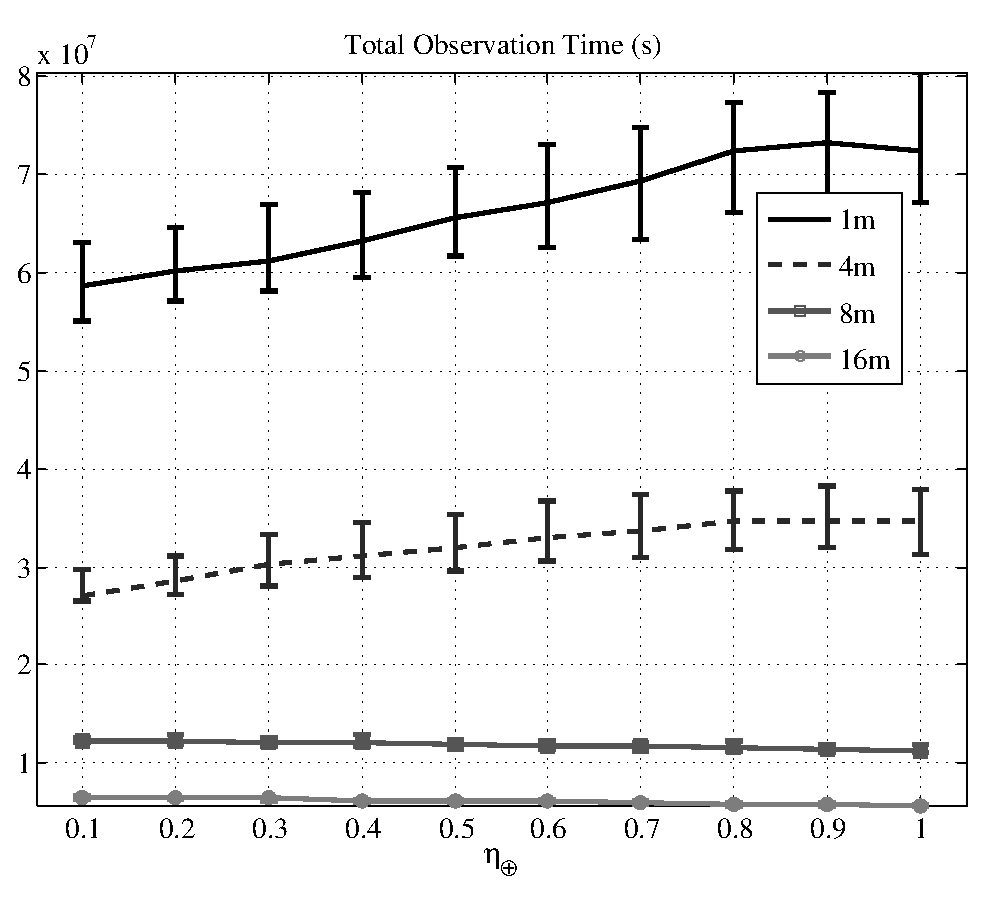
\includegraphics[width=2.8in]{./figures/occulters_obstime}}
\caption[Total observation times]{ \label{fig:obsTimes} Total amount of time spent on planet-finding observations (detections and characterizations) over 5 years for instruments at varying telescope scales.}
 \end{figure}
 
 Similarly, we can compare the efficacy of the two instrument types at providing orbital fits (in this case, defined solely by the number of unique planets that are successfully detected more than 4 times). \reffig{fig:orbFits} demonstrates that in this area, coronagraphs are clearly better than occulters.  Due to the overall higher number of observations coronagraphs can achieve throughout a mission, they have much higher odds of re-detecting the same planet multiple times and can thus produce up to twice as many orbital fits as occulters.
   \begin{figure}[ht]
 \centering
\subfigure[Coronagraphs]{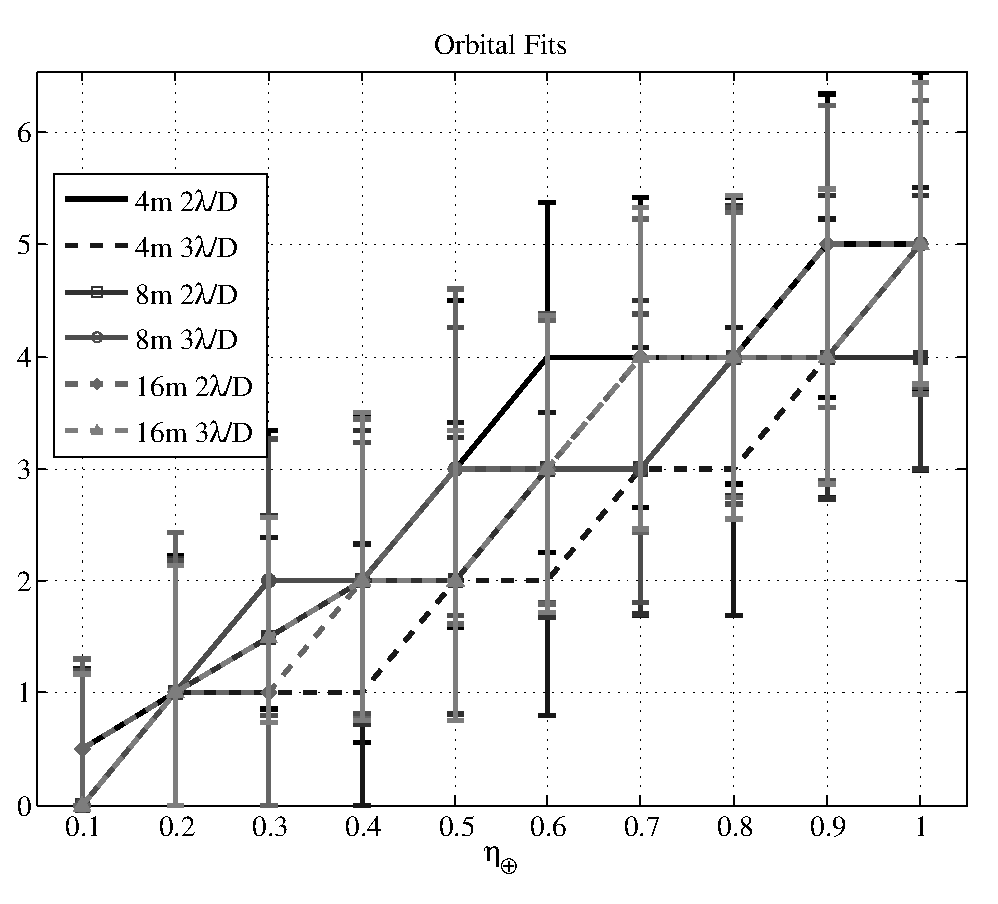
\includegraphics[width=2.85in]{./figures/coronagraphs_norbs}}
\subfigure[MDOs]{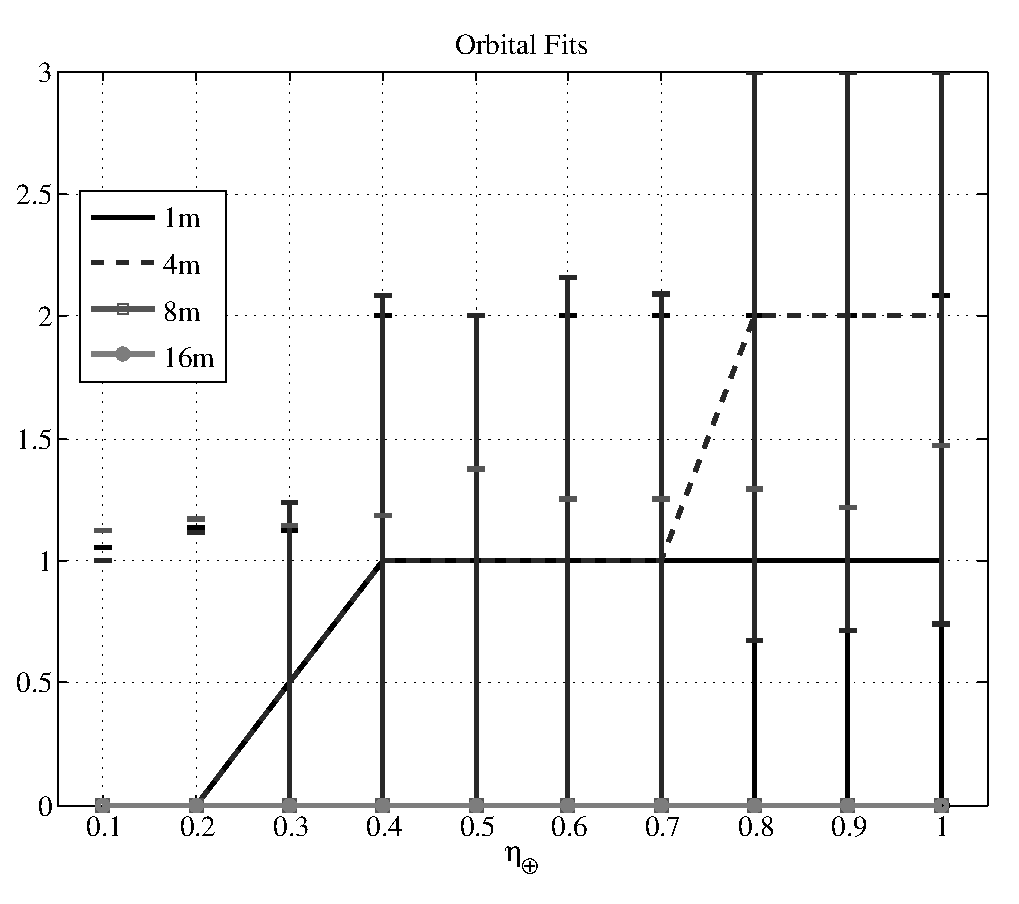
\includegraphics[width=2.9in]{./figures/occulters_norbs}}
\caption[Orbital fits]{ \label{fig:orbFits} Total number of planets observed more than 4 times for instruments at varying telescope scales.}
 \end{figure}  
 
Another point of interest is how quickly we will be able to tell whether an instrument is working as designed.  \reffig{fig:firstDetHists} shows histograms of first planet discoveries as a function of mission time for the 4 and 8 m telescope.  For high values of $\eta_\oplus$, most of the instruments usually have their first detection in the first month of the mission, but as we see in the figure, at $\eta_\oplus = 0.3$, it may take many months before an initial detection.  The two coronagraphs still have their first detections within the first month, but the SDO and MDO designs may take up to 6 months before having the same probability of a first detection.  The results are essentially the same for the 4 and 8m telescope instruments with two interesting exceptions.  The 2 $\lambda/D$ coronagraph appears to actually have a lower probability of a first detection in the first month with an 8 m telescope than with a 4 m telescope.  This is due to the expanded target list available to the 8 m telescope.  Because there are now many more targets to consider, and we've assumed a constant rate of planet occurrence, it is unsurprising that it takes more visits, on average, before a detection is made.  The second interesting feature of these histograms is that the SDO appears to have a higher probability of first detection in the first month than the MDO.  Again, this is due to the available pool of targets and the number of visits made by each.  At the 8 m scale, the MDO is able to make significantly more visits than the SDO.  Since the SDO makes fewer total detections than the MDO, and visits to high completeness stars (which have highest probabilities of detections) occur early in the mission, the SDO at this scale either gets its first detection early on, or much later in the mission during revisits to these stars or at lower completeness targets.  This is evidenced by the large percentage of first detections which occur more than 1 year into the mission for the 8 m SDO.

 \begin{figure}[ht]
 \begin{center}
  \begin{tabular}{c c}
   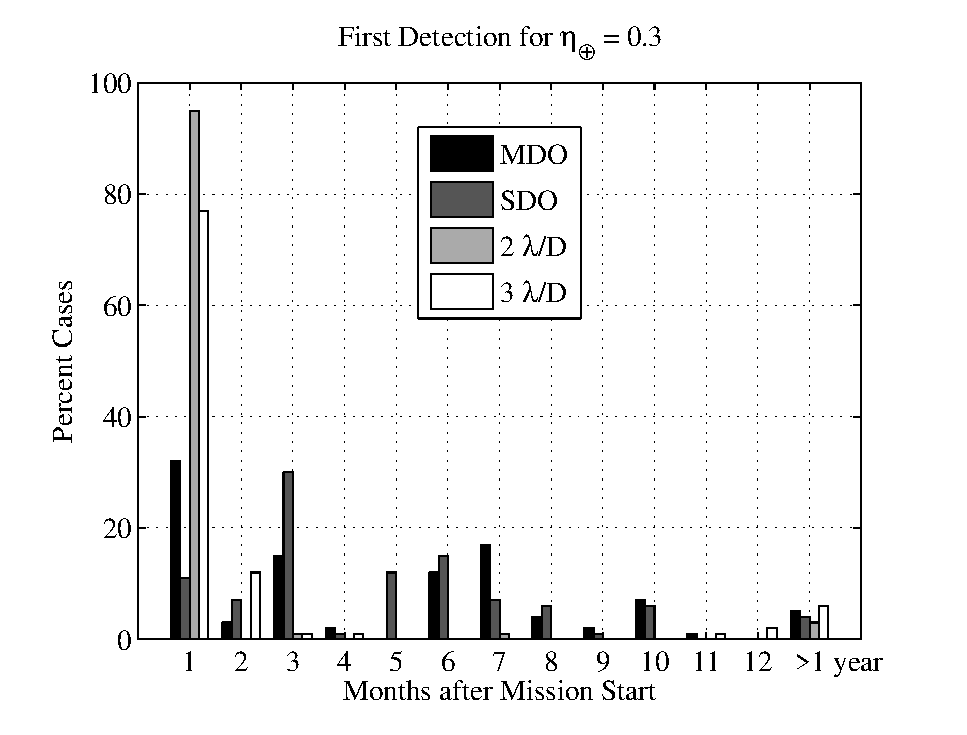
\includegraphics[width=2.9in]{./figures/c4_firstDetHist} &
   \includegraphics[width=2.9in]{./figures/c8_firstDetHist}
   \end{tabular}
 \end{center}
 \caption[First detection histograms]{ \label{fig:firstDetHists} Histograms of first planet detections vs.~months after mission start for the 4m (left) and 8m (right) telescope instrument designs.}
 \end{figure}
 
 \begin{figure}[ht]
 \begin{center}
  \begin{tabular}{c c}
   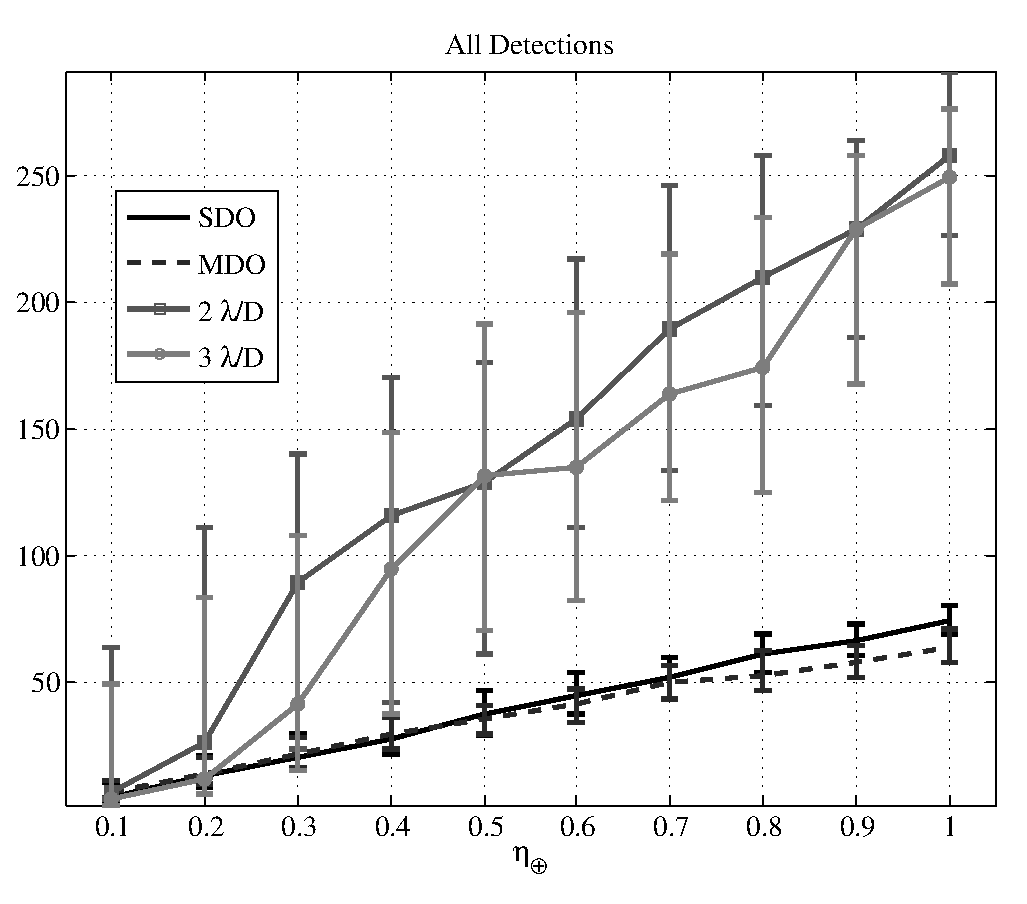
\includegraphics[width=2.9in]{./figures/c4mSE_ADETs} &
   \includegraphics[width=2.9in]{./figures/c4mSE_AuDETs} \\
   \includegraphics[width=2.9in]{./figures/c4mSE_Auvisits} &
   \includegraphics[width=2.9in]{./figures/c4mSE_ASPECTRA}
  \end{tabular}
 \end{center}
 \caption[4 m telescope comparison for super-Earths]{ \label{fig:compinsts4mSE} Simulation results for the SDO, MDO, and the 2 and 3 $\lambda/D$ coronagraph mission concepts as functions of $\eta_\oplus$ with a 4 m telescope for Super-Earth planetary populations..}
 \end{figure}

Besides varying telescope scales, we can also explore the performance of the same instruments on varying planetary populations.  As a first step, we improve slightly on the overly simplistic Earth-twin only population by including habitable zone Super-Earths - rocky planets of 1 to 10 M$_\oplus$ and radii determined by randomly generated ice-rock-iron proportions \citep{fortney2007}. Unsurprisingly, the trends found with this planetary population (\reffig{fig:compinsts4mSE}) are, for the most part, the same as those seen in \reffig{fig:compinsts4m} with an Earth-twin only population, but with larger values for most of the metrics, since Super-Earths are, on average, easier to detect than Earth-twins.  With this population, in terms of unique planet detections, the two occulters and the 2 $\lambda/D$ coronagraph are virtually indistinguishable, with the 3 $\lambda/D$ coronagraph finding about 30\% fewer unique planets.  Due to the larger number of detections (which translates to longer observation times for characterization), a slightly smaller subset of the target list is typically visited than with the Earth-twin only population.  For spectral characterizations, we find that the 3 $\lambda/D$ coronagraph does much better than before, nearly matching the performance of the 2 $\lambda/D$ coronagraph.  Again, this is most likely due to the differing available targets for each, and suggests that the 2 $\lambda/D$ coronagraph's performance in this metric could be improved with scheduling and target selection optimization.

Because O$_3$ does not perform spectral characterizations, but rather band photometry that requires much less integration time it is quite useful in illustrating the effects of certain parameters on the resulting science yield.  As previously discussed, the selection of the target pool is a major variable in the simulation.  Fewer total targets generally increase the total number of detections, while reducing the number of unique detections.  They also increase fuel use for slews, since targets are further apart, on average, and longer burns must be used to keep the mission time below the five year maximum.  In simulations where mission rules only call for photometric characterization in the case of newly discovered planets, the amount of fuel used for stationkeeping is decreased due to the lower number of unique detections. Also, in cases where $\eta_\oplus$ is low, the probability that no planets at all will be detected is increased by decreasing the target pool.  These effects are shown for one of the O$_3$ configurations in \reffig{fig:compComparison}.  Automatically generated target pools (based on minimum completeness) smaller than the ones shown here tend to perform worse in terms of both total and unique detections.  However, it is possible to improve performance by considering not only the single visit completeness of the target systems, but also their placement.  Adding strategically located systems with slightly lower completeness values can actually increase the overall expected number of detections as it leads to smaller average transition slews and a larger number of overall observations.

\begin{figure}[ht]
 \begin{center}
  \begin{tabular}{c c}
   \includegraphics[width=2.9in,clip=true,trim=0.25in 0in 0.5in 0in]{./figures/compComparisonA} &
   \includegraphics[width=2.9in,clip=true,trim=0.25in 0in 0.5in 0in]{./figures/compComparisonB} 
  \end{tabular}
 \end{center}
 \caption[Effects of varying target pools]{ \label{fig:compComparison} Simulation results for O$_3$ with different target pool sizes and Earth-twin systems.  The three values correspond to minimum single visit completeness values of 0.1, 0.2 and 0.3. Mission rules for these simulations called for photometric characterization of newly discovered planets in the Blue band only.}
 \end{figure}

We can also use O$_3$ to analyze what happens when observations are allowed only when the planet is outside strict geometric IWA (90 mas, in this case) as opposed to allowing observations between the petals of the occulter (down to 75 mas).   We also observe the effects of performing photometry in only the blue band or in both bands.  \reffig{fig:comp2} shows that, as expected, missions which attempt photometry in both bands will have fewer detections than mission characterizing only in the blue, due to the time required to change the telescope-occulter distance.  Furthermore, missions which attempt to characterize planets through the occulter's petals do much better in getting red band photometry as the doubled inner working angle at 90 mas makes most HZ planets unobservable.

\begin{figure}[ht!]
 \begin{center}
  \begin{tabular}{c c}
   \includegraphics[width=2.9in,clip=true,trim=0.25in 0in 0.5in 0in]{./figures/comp2A} &
   \includegraphics[width=2.9in,clip=true,trim=0.25in 0in 0.5in 0in]{./figures/comp2B} \\
      \includegraphics[width=2.9in,clip=true,trim=0.25in 0in 0.5in 0in]{./figures/comp2C} &
   \includegraphics[width=2.9in,clip=true,trim=0.25in 0in 0.5in 0in]{./figures/comp2D} 
  \end{tabular}
 \end{center}
 \caption[O$_3$ simulation results]{ \label{fig:comp2} Simulation results for O$_3$ performing Blue or Red + Blue band photometry, and searching for planets down to angular separations of 90 or 75 mas. The much larger difference in the two curves in the final two plots is due to the extreme difficulty of getting complete photometry in the Red band where the geometric IWA is 180 mas for the 90 mas case.}
 \end{figure}
 
\reffig{fig:bpComparison} shows the effects of varying the default burn portion.  Increasing this parameter has the predictable effect of decreasing the number of total detections, while greatly shortening the mission duration.  While this would ordinarily be a reason to maintain a minimum default burn portion, a shorter mission lifetime with almost the same science return may actually be quite attractive when discussing smaller class missions.  Both operating costs  and the probability of single event failure decrease with the mission span, making shorter missions somewhat preferable,  if we could expect an equivalent science return.
 \begin{figure}[ht]
 \begin{center}
  \begin{tabular}{c c}
   \includegraphics[width=2.9in,clip=true,trim=0.25in 0in 0.5in 0in]{./figures/bpComparisonA} &
   \includegraphics[width=2.9in,clip=true,trim=0.25in 0in 0.5in 0in]{./figures/bpComparisonB} 
  \end{tabular}
 \end{center}
 \caption[Effects of varying burn portion]{ \label{fig:bpComparison} Simulation results for different default burn portions using the 2 band photometry, 75 mas IWA O$_3$ configuration.}
 \end{figure}

 \reffig{fig:fuel_use} shows the average propellant use for the simulations of the 4 m SDO and THEIA mission concept.  Both occulters were assumed to have the same initial mass (the payload capacity of an ATLAS V launch vehicle), which translates to a smaller total fuel capacity for the heavier SDO.  As expected, the SDO, having the larger separation distance from the telescope, uses more fuel overall.  It is also instructive to look at the breakdown of fuel use in terms of slewing and stationkeeping.  Because characterizations for THEIA include an extra slew at full thrust, as $\eta_\oplus$ increases so does the number of characterizations and the slew propellant usage.  In the case of the single distance occulter, on the other hand, more time characterizing translates to less time slewing, and so its slew propellant use drops with increasing $\eta_\oplus$.  A similar effect is seen in the stationkeeping propellant use---as $\eta_\oplus$ increases, THEIA spends more and more time at the smaller separation distance, where stationkeeping fuel costs are lower, thereby slightly lowering overall stationkeeping fuel use.  At the same time, the single distance occulter spends more time characterizing at its wider separation, increasing its stationkeeping fuel use.  All of these effects, however, are relatively minor when compared with the difference in the two occulters' dry masses---the fuel remaining at the end of THEIA's primary mission is due almost completely to the fact that the occulter is smaller and lighter than its single distance counterpart.
\begin{figure}[ht]
\centering
 \includegraphics[width=6in,clip=true,trim=0.8in 0in 0.75in 0in]{./figures/theiaFuel}
 \caption[Occulter propellant use]{ \label{fig:fuel_use} Occulter propellant use (in kg) for the 4 m SDO (gray) and THEIA (black). Although the assumed stationkeeping and slewing propulsion systems use different propellants, the simulation does not distinguish between the two fuel types and simply assumes that enough fuel is available, up to a maximum total fuel mass.  When this mass is exceeded, the mission ends, regardless of mission time. The primary cause for the difference in the fuel remaining after 5 years is the difference in starshade dry masses.}
 \end{figure}
 
We can take advantage of the extra fuel at THEIA's disposal by adding an extended mission to make up for some of the differences in science yield between the two occulter designs.  One option is to continue into the extended mission with the same mission rules as for the primary mission.  However, because there is generally only about 2.5 years of fuel left, and the THEIA design is able to find all of the easily observable planets during the primary mission, this approach does not significantly increase overall science yield.  Another alternative is to limit the target list in the extended mission to only those stars which had planets detected in the primary mission.  This allows for many additional detections, and, in some cases, a few more complete spectra.  

\reffig{fig:theia_ext} shows the results for the primary and primary + extended missions.  Unfortunately, for this design, the extended mission does little to increase the number of complete spectra attained, mostly because the characterization times allow for full spectra only for planets that are observable for longer than the average observing season for this population.  This means that if a full spectrum was achievable, it would generally have been acquired in the primary mission.  However, the limited target pool with guaranteed observable planets allows us to significantly increase the total number of detections in a relatively short time.  Enough of these occur at varying points on the planets' orbits that this translates to a significant number of orbital fits for the total mission (up to 5, on average, for $\eta_\oplus = 1$).  In this respect, THEIA is superior to the single distance occulter design.  With the larger occulter, to get the same number of orbital fits, it would be  necessary either to increase the fuel carried (thereby requiring a larger launch vehicle and increasing costs), or to partition the primary mission in this fashion, allocating the last one or two years to only revisiting systems with previous detections, which would sacrifice the total number of unique planets found.

\begin{figure}[ht]
\centering
 \includegraphics[width=6in,clip=true,trim=0.8in 0in 0.75in 0in]{./figures/theiaExt} 
 \caption[THEIA Extended Mission]{ \label{fig:theia_ext} Simulation results for the primary THEIA mission shown and the primary + extended mission, where the occulter is allowed to use all of the available fuel.} 
 \end{figure}
 
 Another area of interest is the effect of varying exo-zodi levels on  mission science yield.  \reffig{fig:intTimesVarZodi} shows the integration times required for THEIA to detect and spectrally characterize a 25 $\Delta$mag Earth-twin about each of 117 target stars, with exo-zodi levels at the mean and 2 $\sigma$ levels of the historical zodi distribution for the solar system (see \reffig{fig:zodi_dist}).
 \begin{figure}[ht]
 \begin{center}
  \begin{tabular}{c c}
   \includegraphics[width=2.9in,clip=true,trim=0.25in 0in 0.45in 0.05in]{./figures/detTimes} &
   \includegraphics[width=2.9in,clip=true,trim=0.25in 0in 0.45in 0.05in]{./figures/charTimes}
   \end{tabular}
 \end{center}
 \caption[Integration times for varying exo-zodi levels]{\label{fig:intTimesVarZodi} Integration times for planetary detection with 0.1\% false positives, and spectral characterizations with S/N = 11 at the 760nm O$_2$ feature with resolving power R = 70.  The planet is assumed to be 25 magnitudes fainter than the target star, and targets are ordered with decreasing magnitude.  The legend numbers are the exo-zodi levels in zodi.}
 \end{figure} 
 These plots illustrate quite well how the different approaches to detection and characterization (bayesian inference vs.~integrating to a pre-determined signal-to-noise ratio) are affected by varying the exo-zodi magnitude with a fixed  planet signal.  Despite the proportionately larger increase in detection integration time for lower magnitude stars these all remain below 30 hours.  On the other hand, the integration times required for characterization quickly stretch to many months, regardless of exo-zodi levels.  From this, we can predict that while increased exo-zodi levels may decrease the number of detections, this effect probably won't be too dramatic unless the exo-zodi is present at much higher levels than found in the historical distribution of the solar system zodi over the last 80 Myr.  At the same time, because the only detections that will lead to complete spectral characterizations will be of bright planets around stars with long observing seasons, the increased characterization integration time should similarly lead to a relatively small decrease in the number of full spectra attained throughout the mission.
 
We can test this hypothesis by running the mission simulations with varying exo-zodi levels.  Doing so for 1.55 and 3.3 zodi produces a difference of 5\%, on average, in the number unique planets found, and 3.5\% in the number of total detections over the course of the mission.  The number of spectra acquired also changes quite modestly, with a difference of 6\%, on average, biased towards simulations with higher frequencies of planets, as shown in \reffig{fig:ASPECTRA_varZ}.
\begin{figure}[ht]
 \begin{center}
   \includegraphics[width=4.5in,clip=true,trim=0.25in 0in 0.5in 0.05in]{./figures/ASPECTRA_varZ}
 \end{center}
 \caption[Spectral characterizations at varying exo-zodi levels]{ \label{fig:ASPECTRA_varZ} Simulation results of spectral characterizations with S/N = 11 at the 760nm O$_2$ feature with resolving power R = 70. The legend numbers are the exo-zodi levels in zodi.}
 \end{figure}
 
 \begin{figure}[ht]
 \begin{center}
  \begin{tabular}{c c}
   \includegraphics[width=2.9in,clip=true,trim=0.25in 0in 0.5in 0.05in]{./figures/obstime_varZ} &
   \includegraphics[width=2.9in,clip=true,trim=0.25in 0in 0.5in 0.05in]{./figures/utargs_varZ}\\
   \includegraphics[width=2.9in,clip=true,trim=0.1in 0in 0.5in 0.05in]{./figures/slewMass_varZ} &
   \includegraphics[width=2.9in,clip=true,trim=0.1in 0in 0.5in 0.05in]{./figures/skMass_varZ}
   \end{tabular}
 \end{center}
 \caption[Effects of varying exo-zodi levels]{ \label{fig:obstime_varZ} Total time for planet-finding/characterizing observations over the length of a mission, the number  target stars observed at least once in the course of the mission, propellant  used for transit slews, and propellant used for stationkeeping for THEIA with varying levels of exo-zodi.}
 \end{figure}
 The most significant differences in the two simulation ensembles occur in the amount of observation time and the number of targets visited.  As shown in Figure \ref{fig:obstime_varZ}, the amount of time spent on planet-finding/characterizing observations increases by two months, on average, between the 1.55 and 3.3 zodi simulations.  While this represents only 3\% of the allotted 5 years, we must keep in mind that for a design featuring a starshade, the majority of the mission time is spent repositioning the starshade between target stars. For THEIA, typically only 20 to 30\% of the mission time is used planetary observations, making this a 10\% increase.  Because of this, the increase in observation time leads to a decrease in the number of targets that can be observed within the primary mission.   Longer observation times for occulters also lead to longer station-keeping times versus transit slew times which can be a very important factor in the mission design.  Since THEIA uses a separate propulsion system for station-keeping, which uses a different type of fuel from the slewing propulsion system, an incorrect assumption as to how much  observation time is required could lead to major problems.  Since the mission cannot proceed without adequate supplies of each propellant type, budgeting too much or too little observation time may lead to the mission ending early.  The differences in observation times due to varying the assumed exo-zodi levels lead to differing requirements on the propellant carried by the starshade.
  
While it seems that as long as exo-zodi levels do not typically exceed those found in our own solar system's past, we should be able to achieve the primary goal of finding and characterizing planets, we will lose some of the science yield associated with observing a larger sample size if exo-zodi levels verge towards the high end of this distribution.  At the same time, any large ambiguity in the expected exo-zodi levels will make mission design and planning much more difficult. If we consider exo-zodi levels outside the 2 $\sigma$ level of the solar system's historical distribution, as expected, all science yield metrics produce lower results.  At 10 zodi concentrations, the mission simulations produce, on average, 19\% fewer unique detections, 17\% fewer total detections, and 26\% fewer spectral characterizations (as compared with the 1.55 zodi simulations).  More significantly, in simulations where Earth-like planets are assumed to be rare ($\eta_\oplus < 0.2$), almost 18\% of all mission simulations have zero spectral characterizations, which means that if high exo-zodi levels are common and planets are rare in our target pool, there is a real danger of being unable to meet a basic mission requirement.

In addition to the possibility of higher overall exo-zodi levels, we also know that dust disks may form concentrations (or `clumps'),  especially in the presence of planetary bodies \citep{stark2008detectability}.  It is unreasonable to assume that our detection integration time algorithm can achieve arbitrarily low false positive rates regardless of any structure in the background, and it is likely that there will be observations where $C_b$ cannot be accurately estimated in the time given by the algorithm described above, or will vary significantly throughout the field of view.  This will lead to an increase in the number of false positives, which will require additional integration time to resolve.

A simple approach to modeling these effects is to increase the number of false positives generated in our simulations, while leaving the same integration times for detections as before.  This approximates the situation where a planet signal is found in the data due to mischaracterization of the background.  In all previous simulations the false positive rate used to calculate detection integration times was also used to generate false positives in the simulations of observations. Now, we decouple these two values, leaving the same low rate for the detection time calculation, but increasing the rate at which false positives are generated in the simulation.

Since THEIA's mission rules require spectral characterization after each new detection, it is assumed that this would resolve any false positives due to exo-zodiacal clumping, at the expense of the wasted integration time. With these simplifying assumptions, we have a system in which false positives generated by bright structures in the exo-zodiacal dust clouds do not directly compete with detections of real planets.  Rather, the time spent spectrally characterizing these false alarms takes away from the time available to find real planets.

\begin{figure}[ht]
 \begin{center}
   \includegraphics[width=2.9in,clip=true,trim=0.25in 0in 0.5in 0.05in]{./figures/AuDETs_zFA}
   \includegraphics[width=2.9in,clip=true,trim=0.25in 0in 0.5in 0.05in]{./figures/ASPECTRA_zFA}
 \end{center}
 \caption[Effects of varying false positive rates.]{ \label{fig:varFA} Comparison of simulations  run with a false positive rate set sufficiently low to produce no false positives, and with a simulated 10\% false positive rate.}
 \end{figure}
The effects of introducing an increased rate of false alarms are very similar to those of increasing the mean exo-zodi level.  When 5\% of observations which were formerly true negatives are made false positives, the number of total detections changes very little, while the number of unique planets found decreases by 3.4\%, while the number of spectral characterizations decreases by about 7.4\%.  Setting the false positive rate at 10\% decreases the number of true detections by 4\%, and the number of unique planets and spectral characterizations by 8.7\% and 16\%, respectively (\reffig{fig:varFA}).  As before, these values reinforce the idea that a planet-finding mission, even for Earth-like planets, is not impossible without detailed prior knowledge of the exo-zodiacal dust distributions of our target stars, although any increase in such knowledge will help greatly in mission design and planning.  

\bigskip
\bigskip

The various results presented here demonstrate the various capabilities of the mission simulation framework described in this chapter.  Most importantly, any new metric that one wishes to evaluate can be calculated from the data generated by these same simulations.  It is not necessary to redo a simulation (unless one wishes to evaluate a new instrument, or a different planet population).  Everything we need to know about a mission can be mined from the data generated in these ensembles.

The simulations developed in this chapter relied heavily upon the models of planetary systems and planet-finding instrumentation developed in the first three chapters.  We can also apply the same models to the problem of data analysis.  The next chapter will demonstrate how the modeling that allowed us to simulate planetary systems can also be used generate exosystem models from observed data.